\chapter{Datenerhebung und Analyse der Algorithmen} \label{datenerhebung_und_analyse}
% Der \gls{accesspoint} sendet die \gls{bssid} und die \gls{ssid}, damit Geräte, wie eine \gls{vm}, sich verbinden können. Algorithmen wie \gls{knn} und \gls{svm} können in einer \gls{api} implementiert werden, um die Datenverarbeitung zu optimieren.

% Für die Untersuchung der Algorithmen und deren Parameter wurde 

% Es werden Testdaten gesammelt, für diese werden dann Vorhersagen getroffen.... Also hier erklären was in dem Kapitel passiert.

% 1. Daten sammeln
% 2. Parameter bestimmt
% 3. 

\section{Aufnahme von WiFi-Fingerprints für die Analyse der Algorithmen} \label{datenerhebung}

% \subsection{Beschreibung der gesammelten Daten}

% Es wird die API ais Kapitel \ref{section-fastapi} verwendet.

% \begin{itemize}
%     \item \textbf{Datenerhebungsmethoden:} Erklären Sie, wie die Daten gesammelt wurden (z.B. welche Geräte, Orte und Zeitpunkte).
%     \item \textbf{Datensätze und Umfang:} Beschreiben Sie den Umfang und die Struktur der gesammelten Datensätze.
%     \item \textbf{Datenqualität und -validität:} Diskutieren Sie die Qualität und Validität der Daten.
% \end{itemize}

Für die Auswertung der Algorithmen und deren Parameter wurden 407 Messungen in 35 Räumen auf dem Campus Wilhelminenhof der Hochschule für Technik und Wirtschaft Berlin (HTW Berlin) in Gebäude C durchgeführt. Die Messungen fanden in dem Zeitraum vom 08. Mai 2024 bis zum 03. Juli 2024 statt und es wurden insgesamt 263 Router erfasst. Für die Aufnahme der WiFi-Fingerprints wurden ein Doogee Y8 und ein Google Pixel 8 Smartphone verwendet.

Die Messungen erfolgten dabei randomisiert, abhängig davon, welche Räume zu dem Zeitpunkt frei waren, und wurden hauptsächlich während der Pausenzeiten und am Abend durchgeführt, da zu diesen Zeiten die meisten Räume zur Verfügung standen. Dabei wurde bewusst darauf verzichtet, den genauen Standort innerhalb der Räume zu planen, um realistische Einsatzbedingungen widerzuspiegeln.

Eine Übersicht der Messungen pro Raum ist in Abbildung \ref{fig:0_general_01} dargestellt.

\begin{figure}[H]
    \centering
    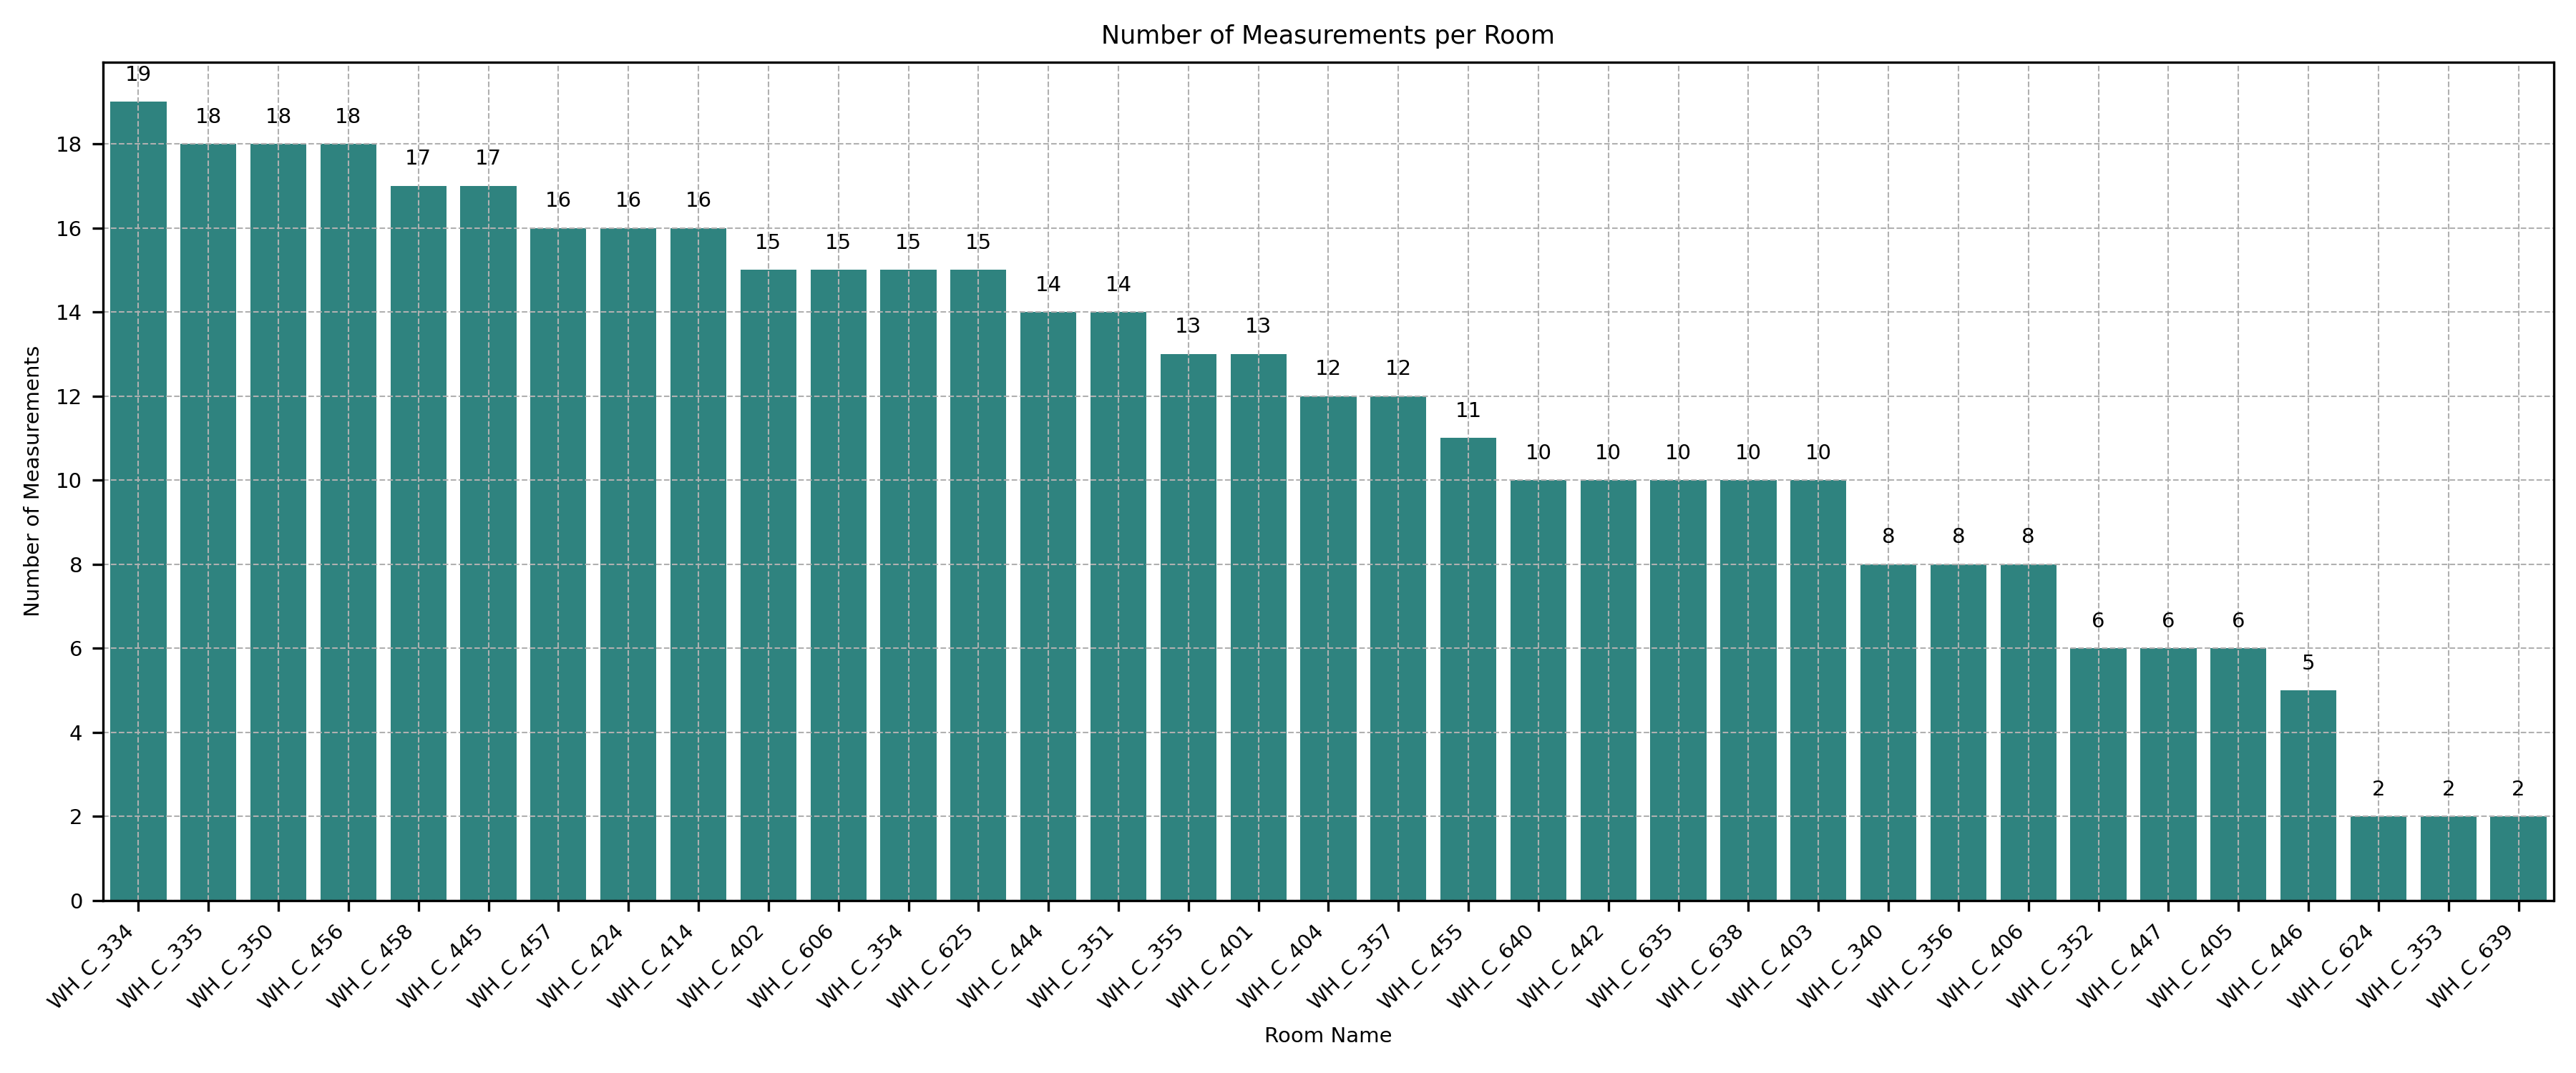
\includegraphics[width=0.8\textwidth]{images/00_general_01.png}
    \caption{Anzahl der Messungen pro Raum}
    \label{fig:0_general_01}
\end{figure}

\section{Beschreibung der Testanwendung} \label{testanwendung}

Für die Untersuchung der Modelle und deren Parameter wurde ein Anwendung in Python entwickelt, welche die verschiedenen Parameter der Algortihmen testet, indem alle möglichen Kombinationen der Parameter an die API gesendet werden und für jede Messung die Vorhersage gespeichert wird. Die Anwendung ist über eine \textit{YAML}-Datei (siehe Code-Beispiel \ref{lst:code_yaml}), in der die grundlegenden Einstellungen, wie die Endpunkte der API, die Anzahl der zu verarbeitenden Messungen und die zu betrachtenden Räume und Flure, definiert werden, konfigurierbar. 

Zudem können unter dem Parameter \textit{parameter\_sets} die verschiedenen Untersuchungsreihen definiert werden. Jeder Eintrag in \textit{parameter\_sets} entspricht einem Testlauf, dessen Ergebnisse unter dem angegebenen Namen in einer \textit{CSV}-Datei gespeichert werden. Innerhalb jedes Eintrags werden die zu testenden Parameter und deren Werte in einem Array angegeben.

In dem Code-Beispiel \ref{lst:code_yaml} sind zwei Testreihen definiert: \textit{01\_knn\_weights} und \textit{08\allowbreak\_router\allowbreak\_pre\-sence\allowbreak\_threshold}. In der ersten Testreihe werden für den \gls{knn}-Algorithmus mit der euklidischen und Sørensen Distanzmetrik und den Werten 5, 7 und 9 für den Parameter \textit{k\_value} die Gewichtungsfunktionen \textit{distance} und \textit{uniform} getestet. In der zweiten Testreihe wurden für den Parameter \textit{router\_presence\_threshold} die Werte 0, 0.25, 0.5 und 0.75 getestet und für die Algorithmen \gls{knn} mit der euklidischen Distanz und den Werten 5, 7 und 9 für den Parameter \textit{k\_value} und \gls{svm} mit dem RBF-Kernel und den Werten 5.0, 1.0 und 0.5 für den Parameter \textit{c\_value} untersucht.

Der Ablauf des Programms ist, dass zunächst die \textit{YAML}-Datei eingelesen, und über alle in den \textit{parameter\_sets} definierten Einträge iteriert wird. Für jeden Eintrag werden alle möglichen Kombinationen der angegebenen Parameter gebildet. Im Fall des zweiten Beispiels ergibt das 24 mögliche Kombinationen, da zwei Algorithmen mit jeweils drei unterschiedlichen Parametern und vier verschiedenen Werten für \textit{router\_presence\_threshold} getestet werden.

Anschließend durchläuft das Programm alle definierten Messungen (in diesem Beispiel 10) und sendet für jede dieser Messungen jede mögliche Parameterkombination über eine \textit{HTTP POST}-Anfrage an die API. Dabei wird auch die ID der jeweiligen Messung über den Parameter \textit{ignore\_measurements} mitgesendet, wodurch sichergestellt wird, dass diese Messung bei der Vorhersage nicht beachtet wird. Dies verhindert, dass die API eine Messung in der Datenbank findet, die exakt dem übermittelten Werten entspricht. Die Resultate der API-Anfragen werden nach dem Durchlauf aller Messungen in einer CSV-Datei, die nach dem Namen des jeweiligen \textit{parameter\_set}-Eintrags benannt ist, gespeichert.

\begin{lstlisting}[caption=\textit{YAML}-Konfigurationsdatei der Testanwendung, label={lst:code_yaml}]
url_fetch: "http://141.45.212.246:8000/measurements/all"
url_predict: "http://141.45.212.246:8000/measurements/predict"

num_measurements: 10
rooms: ["WH_C_351", "WH_C_352", "WH_C_353", "WH_C_335"]
corridors: ["WH_C_35_corridor"]

parameter_sets:
  - name: "01_knn_weights"
    parameters:
      weights: ["distance", "uniform"]
      algorithm:
        knn_euclidean:
          k_value: [5, 7, 9]
        knn_sorensen:
          k_value: [5, 7, 9]
  - name: "08_router_presence_threshold"
    parameters:
      router_presence_threshold: [0, 0.25, 0.5, 0.75]
      algorithm:
        knn_euclidean:
          k_value: [5, 7, 9]
        svm_rbf:
          c_value: [ 5.0, 1.0, 0.5]
\end{lstlisting}

\section{Analyse der Algorithmen und Parameter} \label{untersuchungen}

In dem folgenden Kapitel werden die verschiedenen Algorithmen und deren Parameter miteinander verglichen. Dafür wurde mithilfe der in Kapitel \ref{testanwendung} vorgestellten Anwendung für jede Untersuchung ein Eintrag in der \textit{YAML}-Konfigurationsdatei erstellt und es wurde für alle untersuchten Parameter und jede der 407 Messungen eine Vorhersage getroffen. 

\subsection{Voruntersuchung der nicht im Deatil betrachteten Parameter}

Da in dieser Arbeit für jeden Algorithmus ein Parameter im Detail untersucht wird und für jeden Algorithmus mehrere Parameter existieren, werden im ersten Schritt die Parameter untersucht, die nicht im Detail betrachtet werden. Das sind bei dem \gls{knn}-Modell der \texttt{weights} Parameter, der die Gewichtungsfunktion angibt, bei dem \gls{svm}-Modell mit dem RBF-Kernel der \texttt{gamma} Parameter und bei dem Random Forest Modell sind es die Parameter \textit{max\_depth} und \textit{n\_estimators}.

In Abbildung \ref{fig:1_distance_uniform_weights_01} sind die Ergebnisse des gewichteten und des ungewichteten \gls{knn}-Algorithmus in Abhängigkeit der Anzahl an Messungen pro Raum dargestellt. Wie zu erkennen ist, steigt die Genauigkeit mit der Anzahl an Messungen pro Raum, wobei der Unterschied zwischen \texttt{weights = distance} und \texttt{weights = uniform} mit zunehmender Anzahl an Messungen abnimmt und mit \texttt{weights = distance} bessere Ergebnisse erzielt werden konnten, wenn nur wenige Messungen vorhanden sind. Aus diesem Grund wurde sich dafür entschieden für die weiteren Untersuchungen den \texttt{weights} Parameter auf \texttt{distance} zu setzen.

\begin{figure}[H]
    \centering
    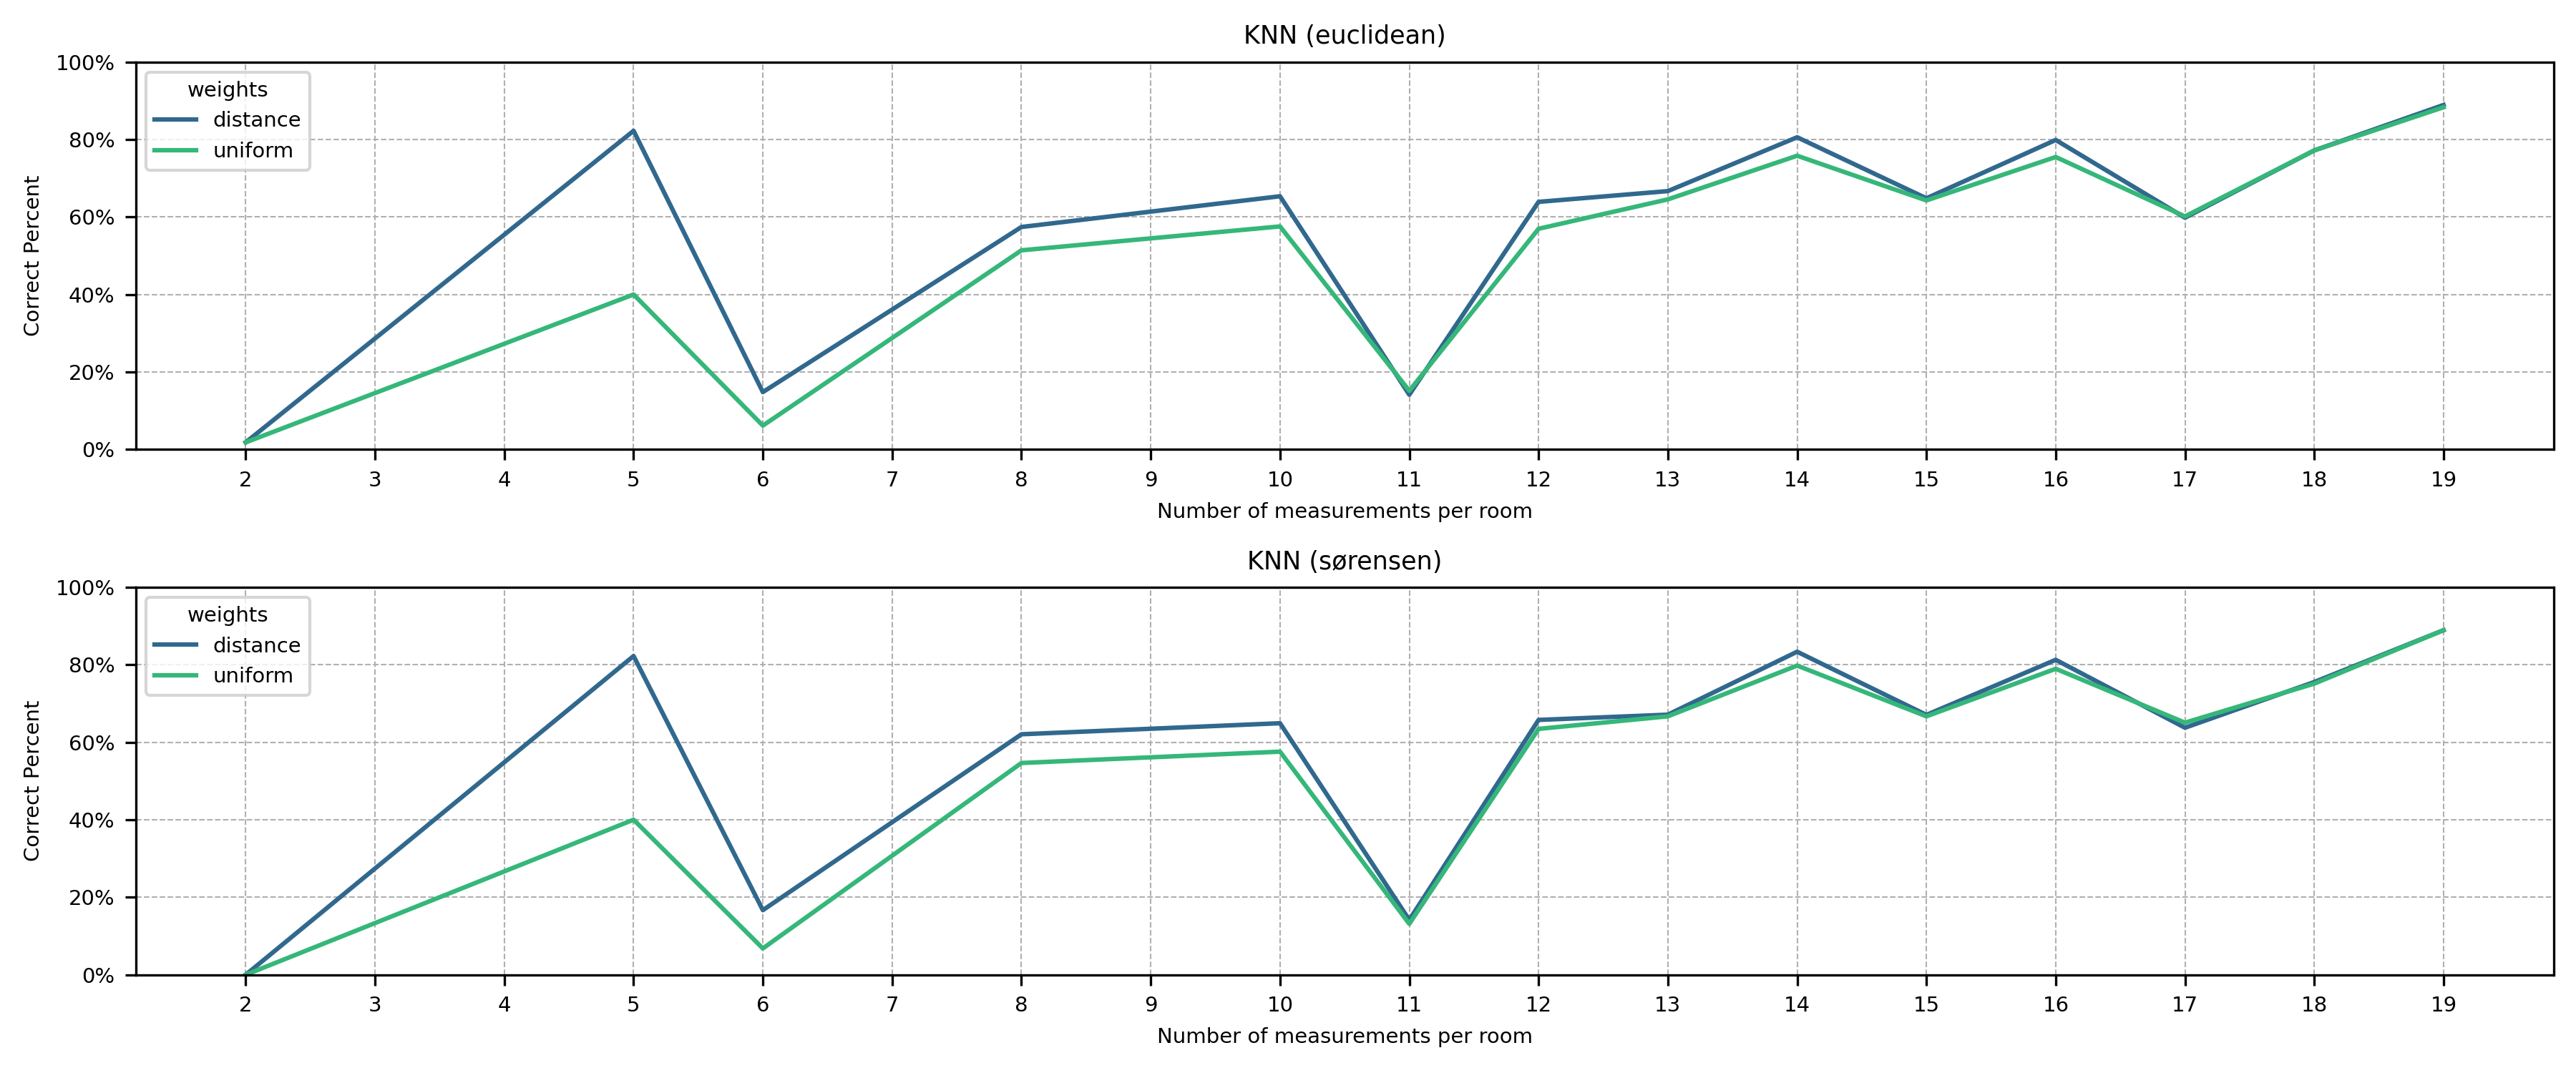
\includegraphics[width=0.8\textwidth]{images/01_knn_weights_01.png}
    \caption{Vergleich des gewichteten (\texttt{weights = distance}) und ungewichteten \gls{knn}-Algorithmus (\texttt{weights = uniform})}
    \label{fig:1_distance_uniform_weights_01}
\end{figure}


Bei dem \gls{svm} Algorithmus wurde der Parameter \texttt{gamma} untersucht, welcher nur für den RBF-Kernel gesetzt werden kann. Dabei wurde die Standardeinstellung von \texttt{scikit-learn}, welche \texttt{scale} ist, mit der Einstellung \texttt{auto} verglichen. Bei \texttt{scale} wird \texttt{gamma} auf

\begin{equation}
    \gamma = \frac{1}{n_{\text{features}} \cdot \text{Var}(X)}
\end{equation}

gesetzt und bei \texttt{auto} auf

\begin{equation}
    \gamma = \frac{1}{n_{\text{features}}}.
\end{equation}


\begin{figure}[H]
    \centering
    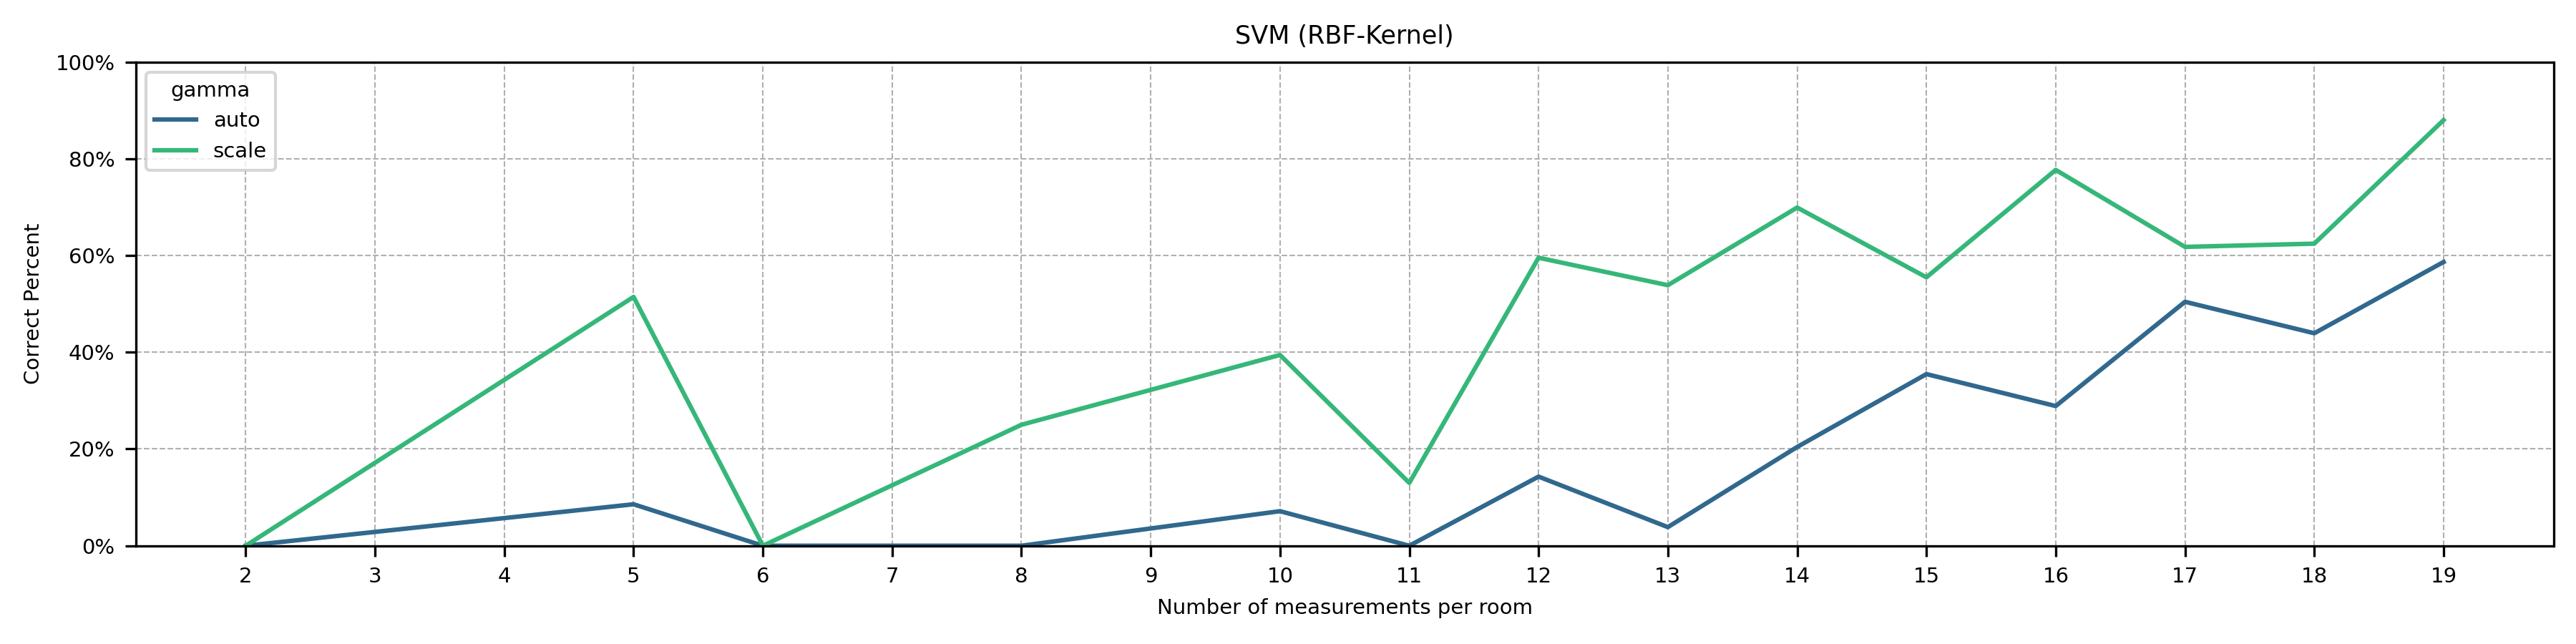
\includegraphics[width=0.8\textwidth]{images/02_svm_gamma_value_01.png}
    \caption{Vergleich der Parameter \texttt{auto} und \texttt{scale} des \texttt{gamma}-Parameters für den \gls{svm}-Algorithmus mit RBF-Kernel}
    \label{fig:1_best_parameters_svm_01}
\end{figure}

In Abbildung \ref{fig:1_best_parameters_svm_01} sind die Ergebnisse der beiden \texttt{gamma} Parameter in Abhängigkeit der Anzahl der Messungen pro Raum dargestellt. Wie zu erkennen ist, ist die Genauigkeit bei \texttt{scale} besser als bei \texttt{auto}. Aus diesem Grund wurde sich dafür entschieden für die weiteren Untersuchungen den \texttt{gamma} Parameter auf \texttt{scale} zu setzen.

% TODO: In welchem Wertebereich liegen die Werte?

% TODO:
% \begin{itemize}
%     \item Es muss auch irgendwo stehen was der average und der weighted average ist und warum beides in den Plots gezeigt wird!
% \end{itemize}

Bei Random Forest werden die beiden Parameter \texttt{max\_depth} (maximale Tiefe der Entscheidungsbäume) und \texttt{n\_estimators} (Anzahl der Entscheidungsbäume) untersucht, da diese laut dem Paper \textit{WiFi Indoor Localization with CSI Fingerprinting-Based Random Forest} neben dem Parameter \texttt{max\_features} (maximale Anzahl der verwendeten Features) den zweit- und drittgrößten Einfluss auf die Genauigkeit haben.\myfootcite{Wang2018WiFiLocalization}{S. 18}

Bei der Untersuchung der maximalen Tiefe der Entscheidungsbäume wurden für den Parameter \texttt{max\_depth} die Werte 1, 3, 5, 7, 9, 11, 13, 15, 17, 19, 21 und \texttt{None} verglichen. Grundlage für diese Entscheidung ist das Paper \textit{WiFi Indoor Localization with CSI Fingerprinting-Based Random Forest}, welches zu dem Ergebnis kam, dass die Genauigkeit der Ergebnisse ab einer bestimmten Tiefe der Entscheidungsbäume stagniert. Der Parameter \texttt{None} wurde zudem verwendet, da dies die Standardimplementierung von \texttt{scikit-learn} ist.\myfootcite{Wang2018WiFiLocalization}{S. 19}\textsuperscript{,}\mycitefoot{scikitlearnRandomForestClassifier}

\begin{figure}[H]
    \centering
    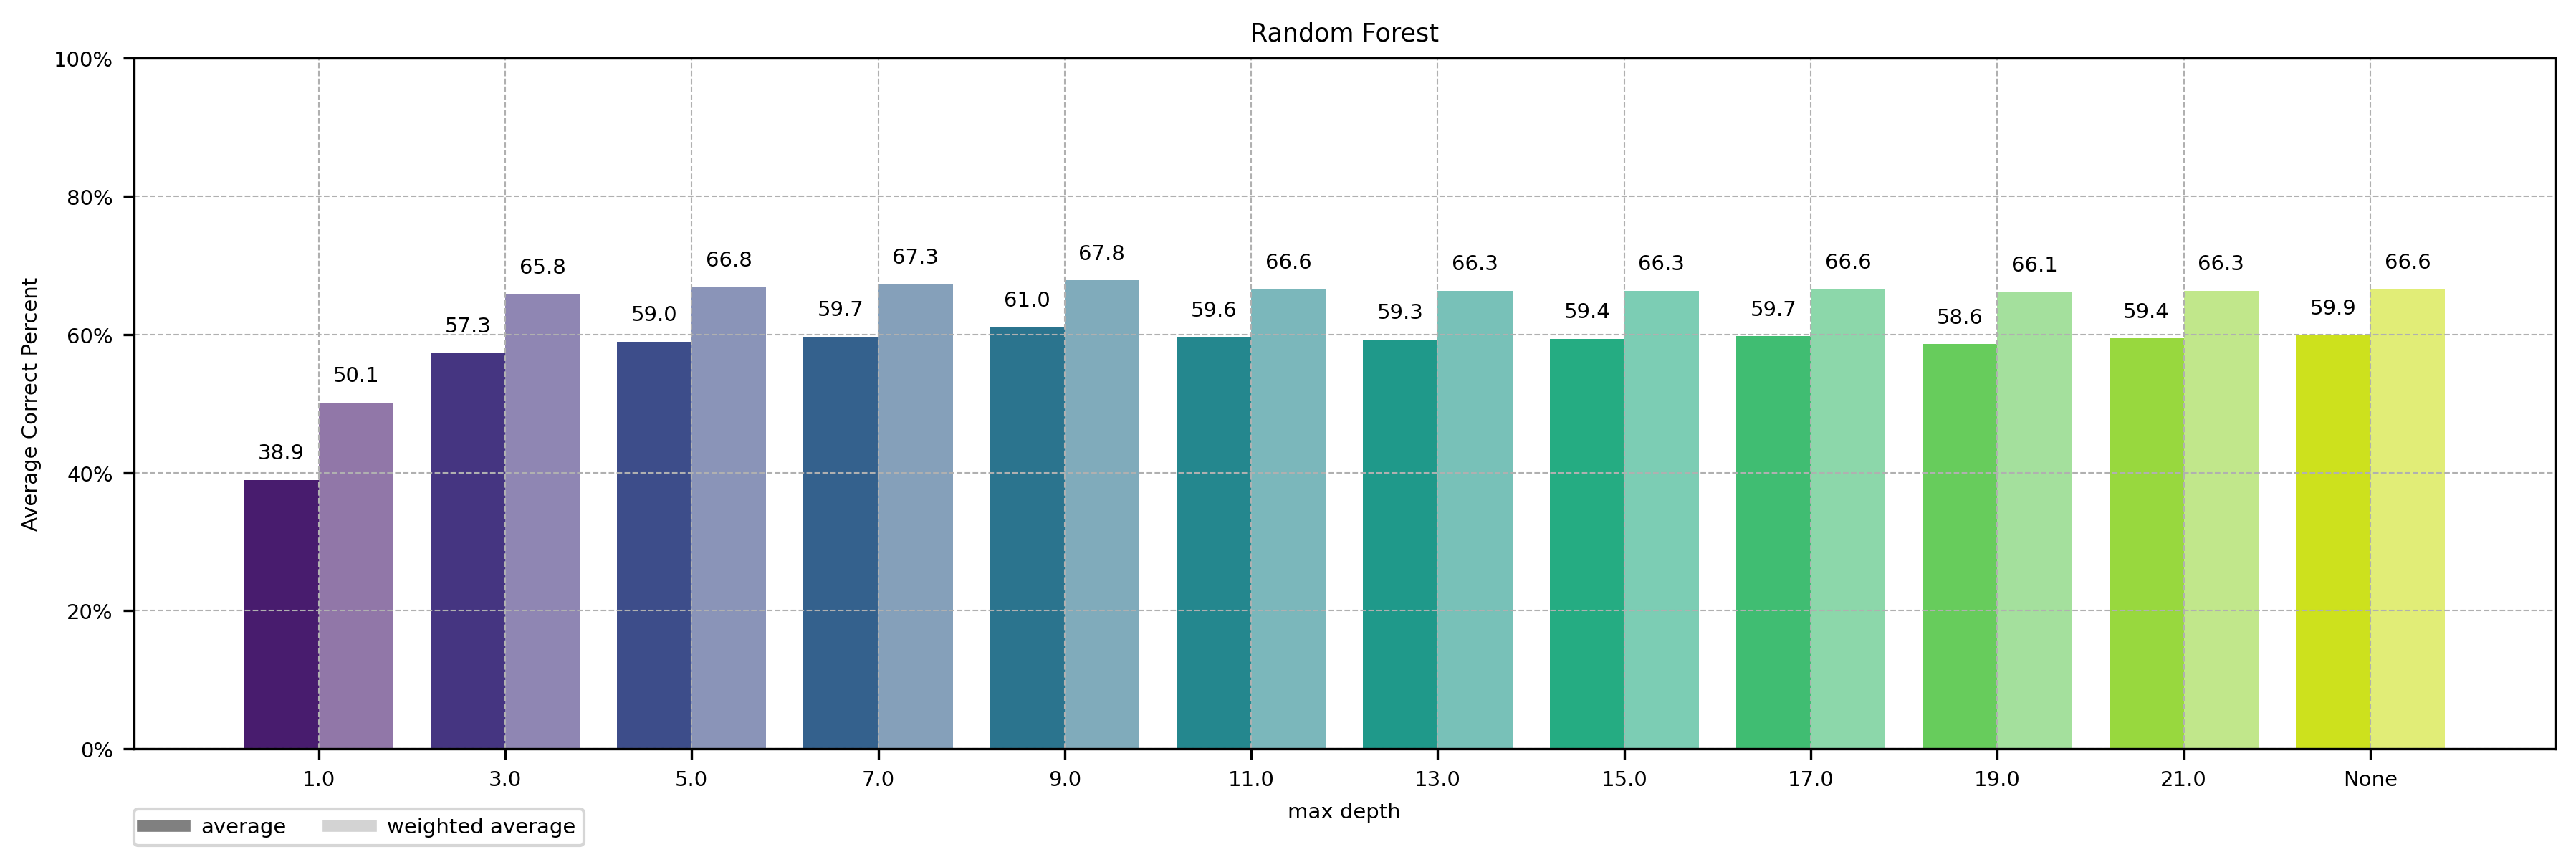
\includegraphics[width=0.8\textwidth]{images/03_random_forest_max_depth_03.png}
    \caption{Vergleich der verschiedenen Werte des \texttt{max\_depth} Parameters für den Random Forest Algorithmus}
    \label{fig:03_random_forest_max_depth_03}
\end{figure}

Wie in Abbildung \ref{fig:03_random_forest_max_depth_03} zu erkennen ist, hat die Wahl des Parameters nur einen geringen Einfluss auf die Genauigkeit der Ergebnisse, mit Ausnahme der Fälle, bei denen \texttt{max\_depth} auf 1 gesetzt ist. Bei allen anderen Werten sind die Genauigkeitsunterschiede minimal. Bei den ungewichteten Ergebnissen beträgt die maximale Abweichung 3,7 \%, während sie bei den gewichteten Ergebnissen bei 2 \% liegt.

Da die Genauigkeit ab einem bestimmten Wert des \texttt{max\_depth} Parameters keine signifikanten Unterschiede mehr aufweist und die besten Ergebnisse bei einer Teife von 9 erzielt werden konnte, wurde sich dafür entschieden für die weiteren Untersuchungen diesen Parameter auf 9 zu setzen.

% Random Forest (n\_estimators):

Bei der Auswahl der Anzahl der Bäume (\texttt{n\_estimators}) wurden die Werte in dem Wertebereich von 10 bis 100 in 10er-Schritten und die Werte in dem Wertebereich zwischen 100 und 1000 in 100er-Schritten untersucht. Diese Auswahl basiert auf den Erkenntnissen des Papers \textit{WiFi Indoor Localization with CSI Fingerprinting-Based Random Forest}, welches zeigt, dass die Genauigkeit mit zunehmender Anzahl an Bäumen zwar steigt, die Rechenzeit jedoch ebenfalls linear mit der Anzahl der Bäume wächst. Das Paper stellt außerdem fest, dass ab einer bestimmten Anzahl an Bäumen keine signifikanten Verbesserungen der Genauigkeit mehr erzielt werden und dass die Unterschiede bei einer geringen Anzahl von Bäumen größer sind.\myfootcite{Wang2018WiFiLocalization}{S. 19}

\begin{figure}[H]
    \centering
    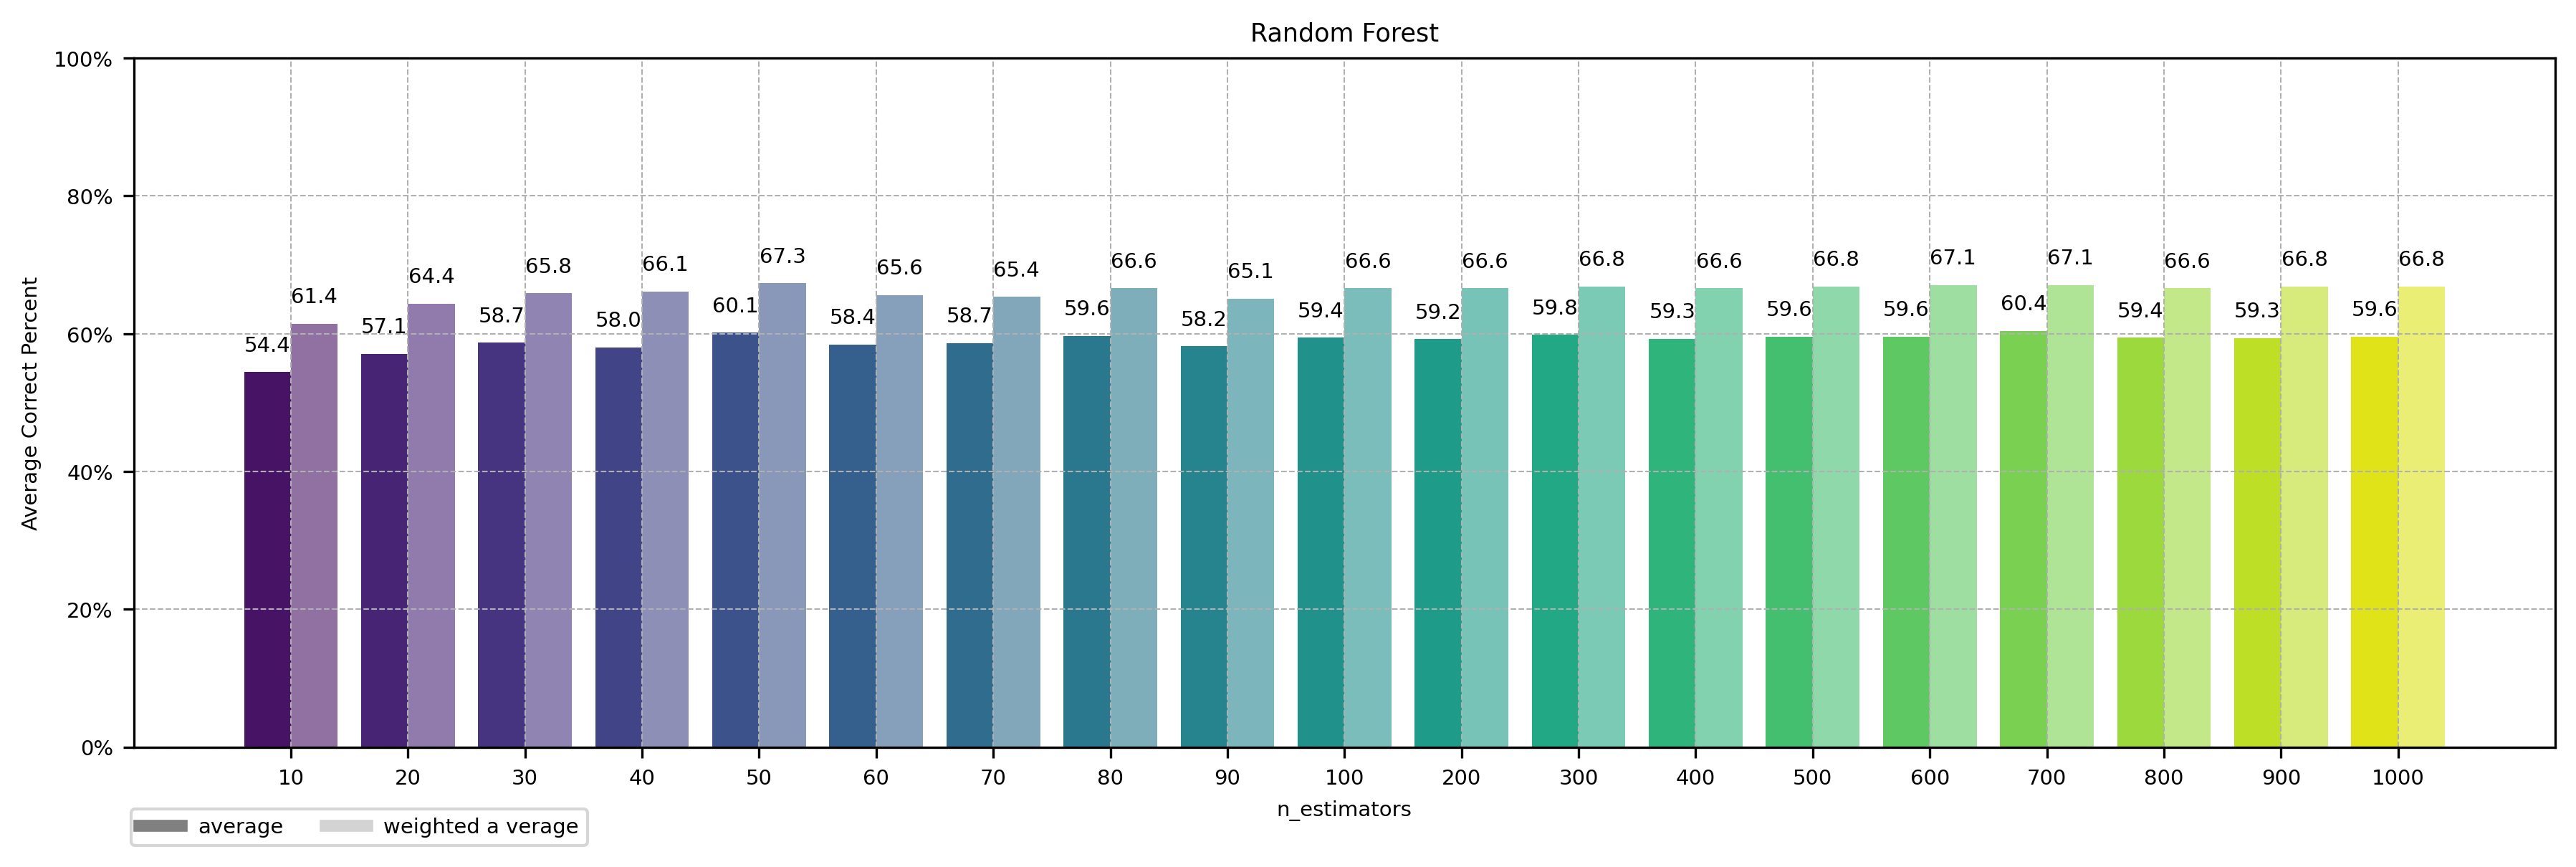
\includegraphics[width=0.8\textwidth]{images/04_random_forest_n_estimators_03.png}
    \caption{Vergleich der verschiedenen Werte des \texttt{n\_estimators} Parameters für den Random Forest Algorithmus}
    \label{fig:04_random_forest_n_estimators_03}
\end{figure}

\begin{figure}[H]
    \centering
    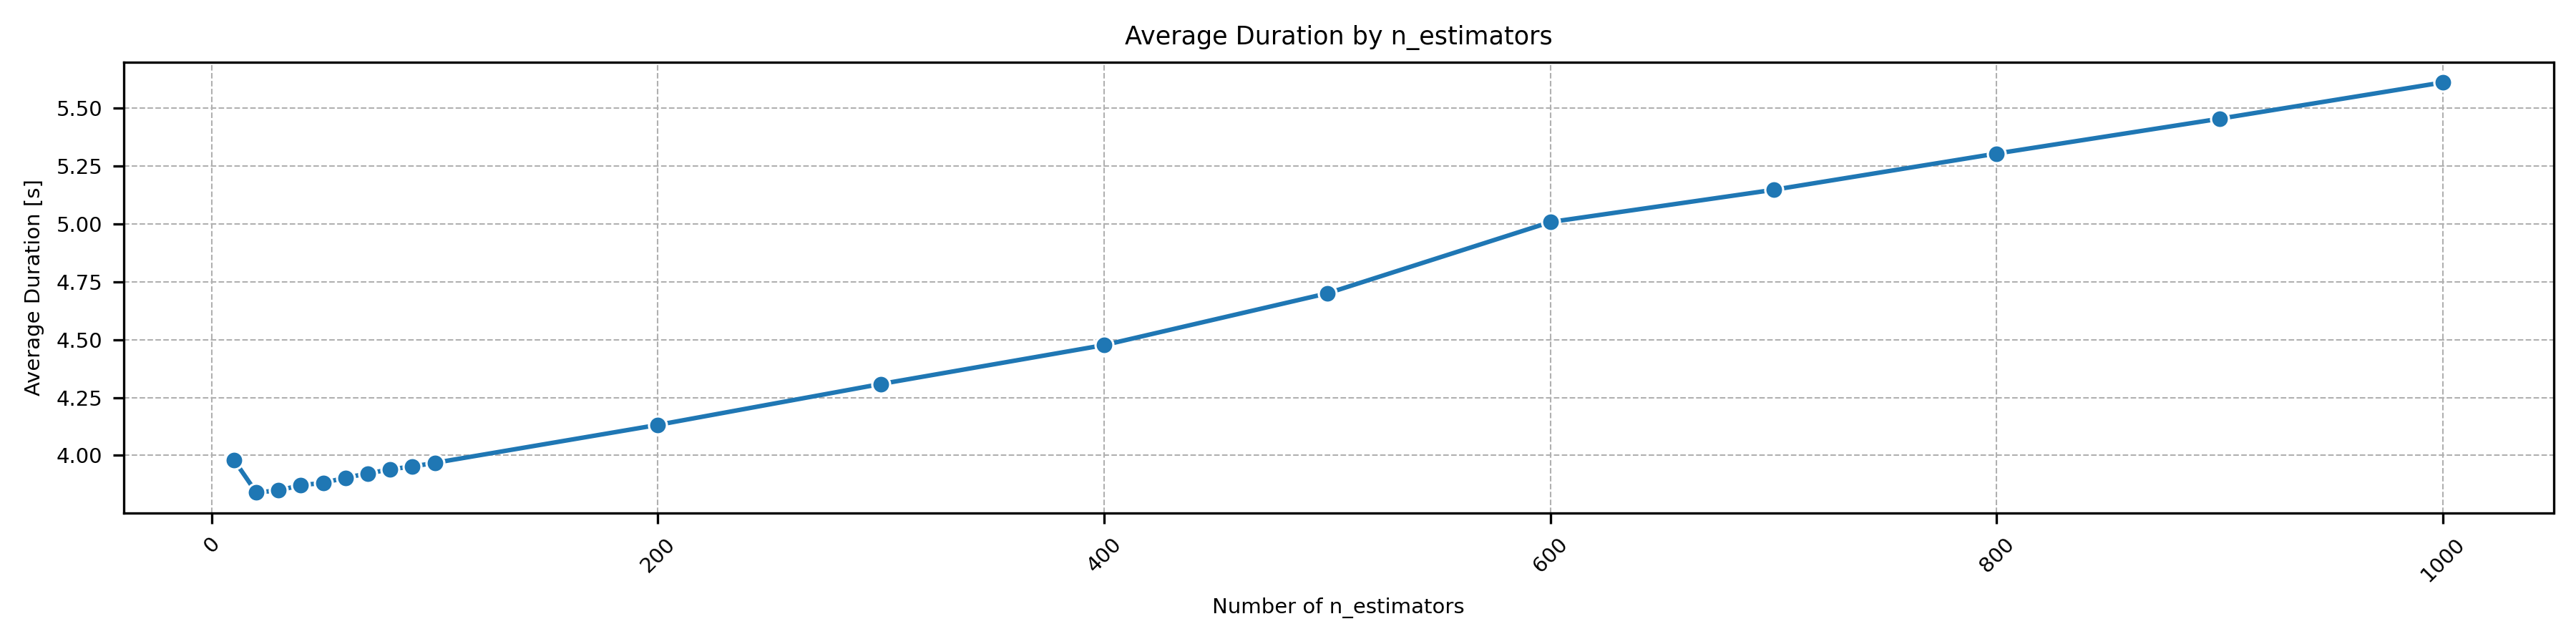
\includegraphics[width=0.8\textwidth]{images/04_random_forest_n_estimators_04.png}
    \caption{Vergleich der Dauer des Random Forest Algorithmus in Abhängigkeit der Anzahl der Bäume}
    \label{fig:04_random_forest_n_estimators_04}
\end{figure}

Wie in Abbildung \ref{fig:04_random_forest_n_estimators_03} zu erkennen ist, hat die Anzahl der Bäume, abgesehen von den kleineren Werten 10 und 20, keinen signifikanten Einfluss auf die Genauigkeit der Ergebnisse. Selbst bei den kleineren Werten ist der Unterschied der Genauigkeit nur minimal, wobei eine Steigerung der Anzahl der Bäume tendenziell zu einer höheren Genauigkeit führt. Die besten Ergebnisse wurden mit 50 Bäumen (60,1 \% ungewichteter Durchschnitt und 67,3 \% gewichteter Durchschnitt) und 700 Bäumen (60,4 \% ungewichteter Durchschnitt und 67,1 \% gewichteter Durchschnitt) erzielt.

In Übereinstimmung mit den Ergebnissen des zitierten Papers, zeigt Abbildung \ref{fig:04_random_forest_n_estimators_04}, dass die Rechenzeit linear mit der Anzahl der Bäume ansteigt. Aufgrund dieser Tatsache und der Tatsache dass die Unterschiede in der Genauigkeit zwischen 50 und 700 Bäumen gering sind, wurde sich dafür entschieden, für die weiteren Untersuchungen die Anzahl der Bäume auf 50 zu setzen.

\subsection{Untersuchung der im Deatil betrachteten Parameter}

Für die detailierten Untersuchungen der Parameter wurden für jeden Algorithmus die drei Parameter ermittelt, die in den meisten Fällen eine richtige Vorhersage getroffen haben. Dafür wurden für den \gls{knn} Algorithmus der Parameter k untersucht, für den Random Forest Algorithmus die Parameter \texttt{max\_features} und für den \gls{svm} Algorithmus der Parameter C. 


Bei dem \gls{knn} Algorithmus mit der Sørensen und euklidischen Distanz wurden jeweils die Parameterwerte 1, 3, 5, 7, 9, 11, 13, 15 getestet, da empfolen wird für k ungerade Werte zu verwenden. Für den \gls{svm} Algorithmus wurden für den linearen- und den RBF-Kernel die Parameterwerte  0.001, 0.005, 0.01, 0.05, 0.1, 0.5, 1, 5 für C verwendet, da diese in dem Paper \textit{Supervised Learning-Based Indoor Positioning System Using WiFi Fingerprints} empfolen wurden.\myfootcite{supervisedLearningIndoorPositioning}{S. 62} Für den Random Forest Algorithmus wurden die Parameterwerte \textit{sqrt}, \textit{log2}, \textit{None}, 0.1, 0.2, 0.3, 0.4, 0.5, 0.6, 0.7, 0.8, 0.9, 1, 2, 3, 4, 5, 6, 7, 8, 9, 10 verglichen, da für den Parameter \texttt{max\_features} in der \textit{scikit-learn} Implementierung des Random Forest Algorithmus die Anzahl der Features als absoluter Wert (Parameterwert 1 bis 10) oder als relativer Wert in Abhängigkeit der Gesamtzahl an Features angegeben werden kann und beides untersucht werden soll. Die Werte 0,1 bis 0,9 entsprechen dabei der Prozentzahl der betrachteten Features und \textit{sqrt} und \textit{log2} entsprechen der Quadratwurzel bzw. dem Logarithmus zur Basis 2 der Gesamtanzahl an Features.


% scikitlearnRandomForestClassifier

% In Abbildung \ref{fig:2_best_parameters_01} sind die besten Parameter für die Algorithmen in Abhängigkeit der Anzahl der Messungen dargestellt. Die Parameter wurden durch die Anwendung des Testprogramms auf die gesammelten Daten ermittelt. Die Parameter wurden so gewählt, dass die Genauigkeit der Algorithmen maximiert wurde. In Abbildung \ref{fig:2_best_parameters_02} ist die durchschnittliche Genauigkeit der Parameter dargestellt. Die Genauigkeit wurde durch die Anwendung des Testprogramms auf die gesammelten Daten ermittelt.

In Abbildung \ref{fig:05_best_parameters_all_01} sind die Ergebnisse der verschiedenen Parameter für den \gls{knn} und \gls{svm} Algorithmus in Abhängigkeit von der Anzahl der Messungen pro Raum dargestellt. Es ist ersichtlich, dass alle Algorithmen bei 5 Messungen pro Raum verhältnismäßig gute Ergebnisse erzielen konnten, während hingegen bei 11 Messungen pro Raum vergleichsweise schlechtere Ergebnisse auftraten. Dies könnte auf einzelne Ausreißer oder Messfehler zurückzuführen sein. Ebenso ist es möglich, dass die Räume mit 5 Messungen unter besonders günstigen Bedingungen erfasst wurden. Nimmt man diese Ausreißer heraus, zeigt sich bei allen Algorithmen die Tendenz, dass die Genauigkeit der korrekten Raumvorhersage mit einer zunehmenden Anzahl an Messungen pro Raum steigt.

In Abbildung \ref{fig:05_best_parameters_all_03} sind die durchschnittlichen Genauigkeiten der Parameter dargestellt. Dabei wurde einmal der Durchschnitt aller Ergebnisse berechnet (\textit{average}) und einmal der gewichtete Durchschnitt (\textit{weighted average}), bei dem für jede Anzahl an Messungen pro Raum der Durchschnitt gebildet wurde und anschließend der Gesamtdurchschnitt. Dies soll einer möglichen Verzerrung entgegenwirken, da so Räume mit mehr Messungen nicht stärker ins Gewicht fallen.

\begin{figure}[H]
    \centering
    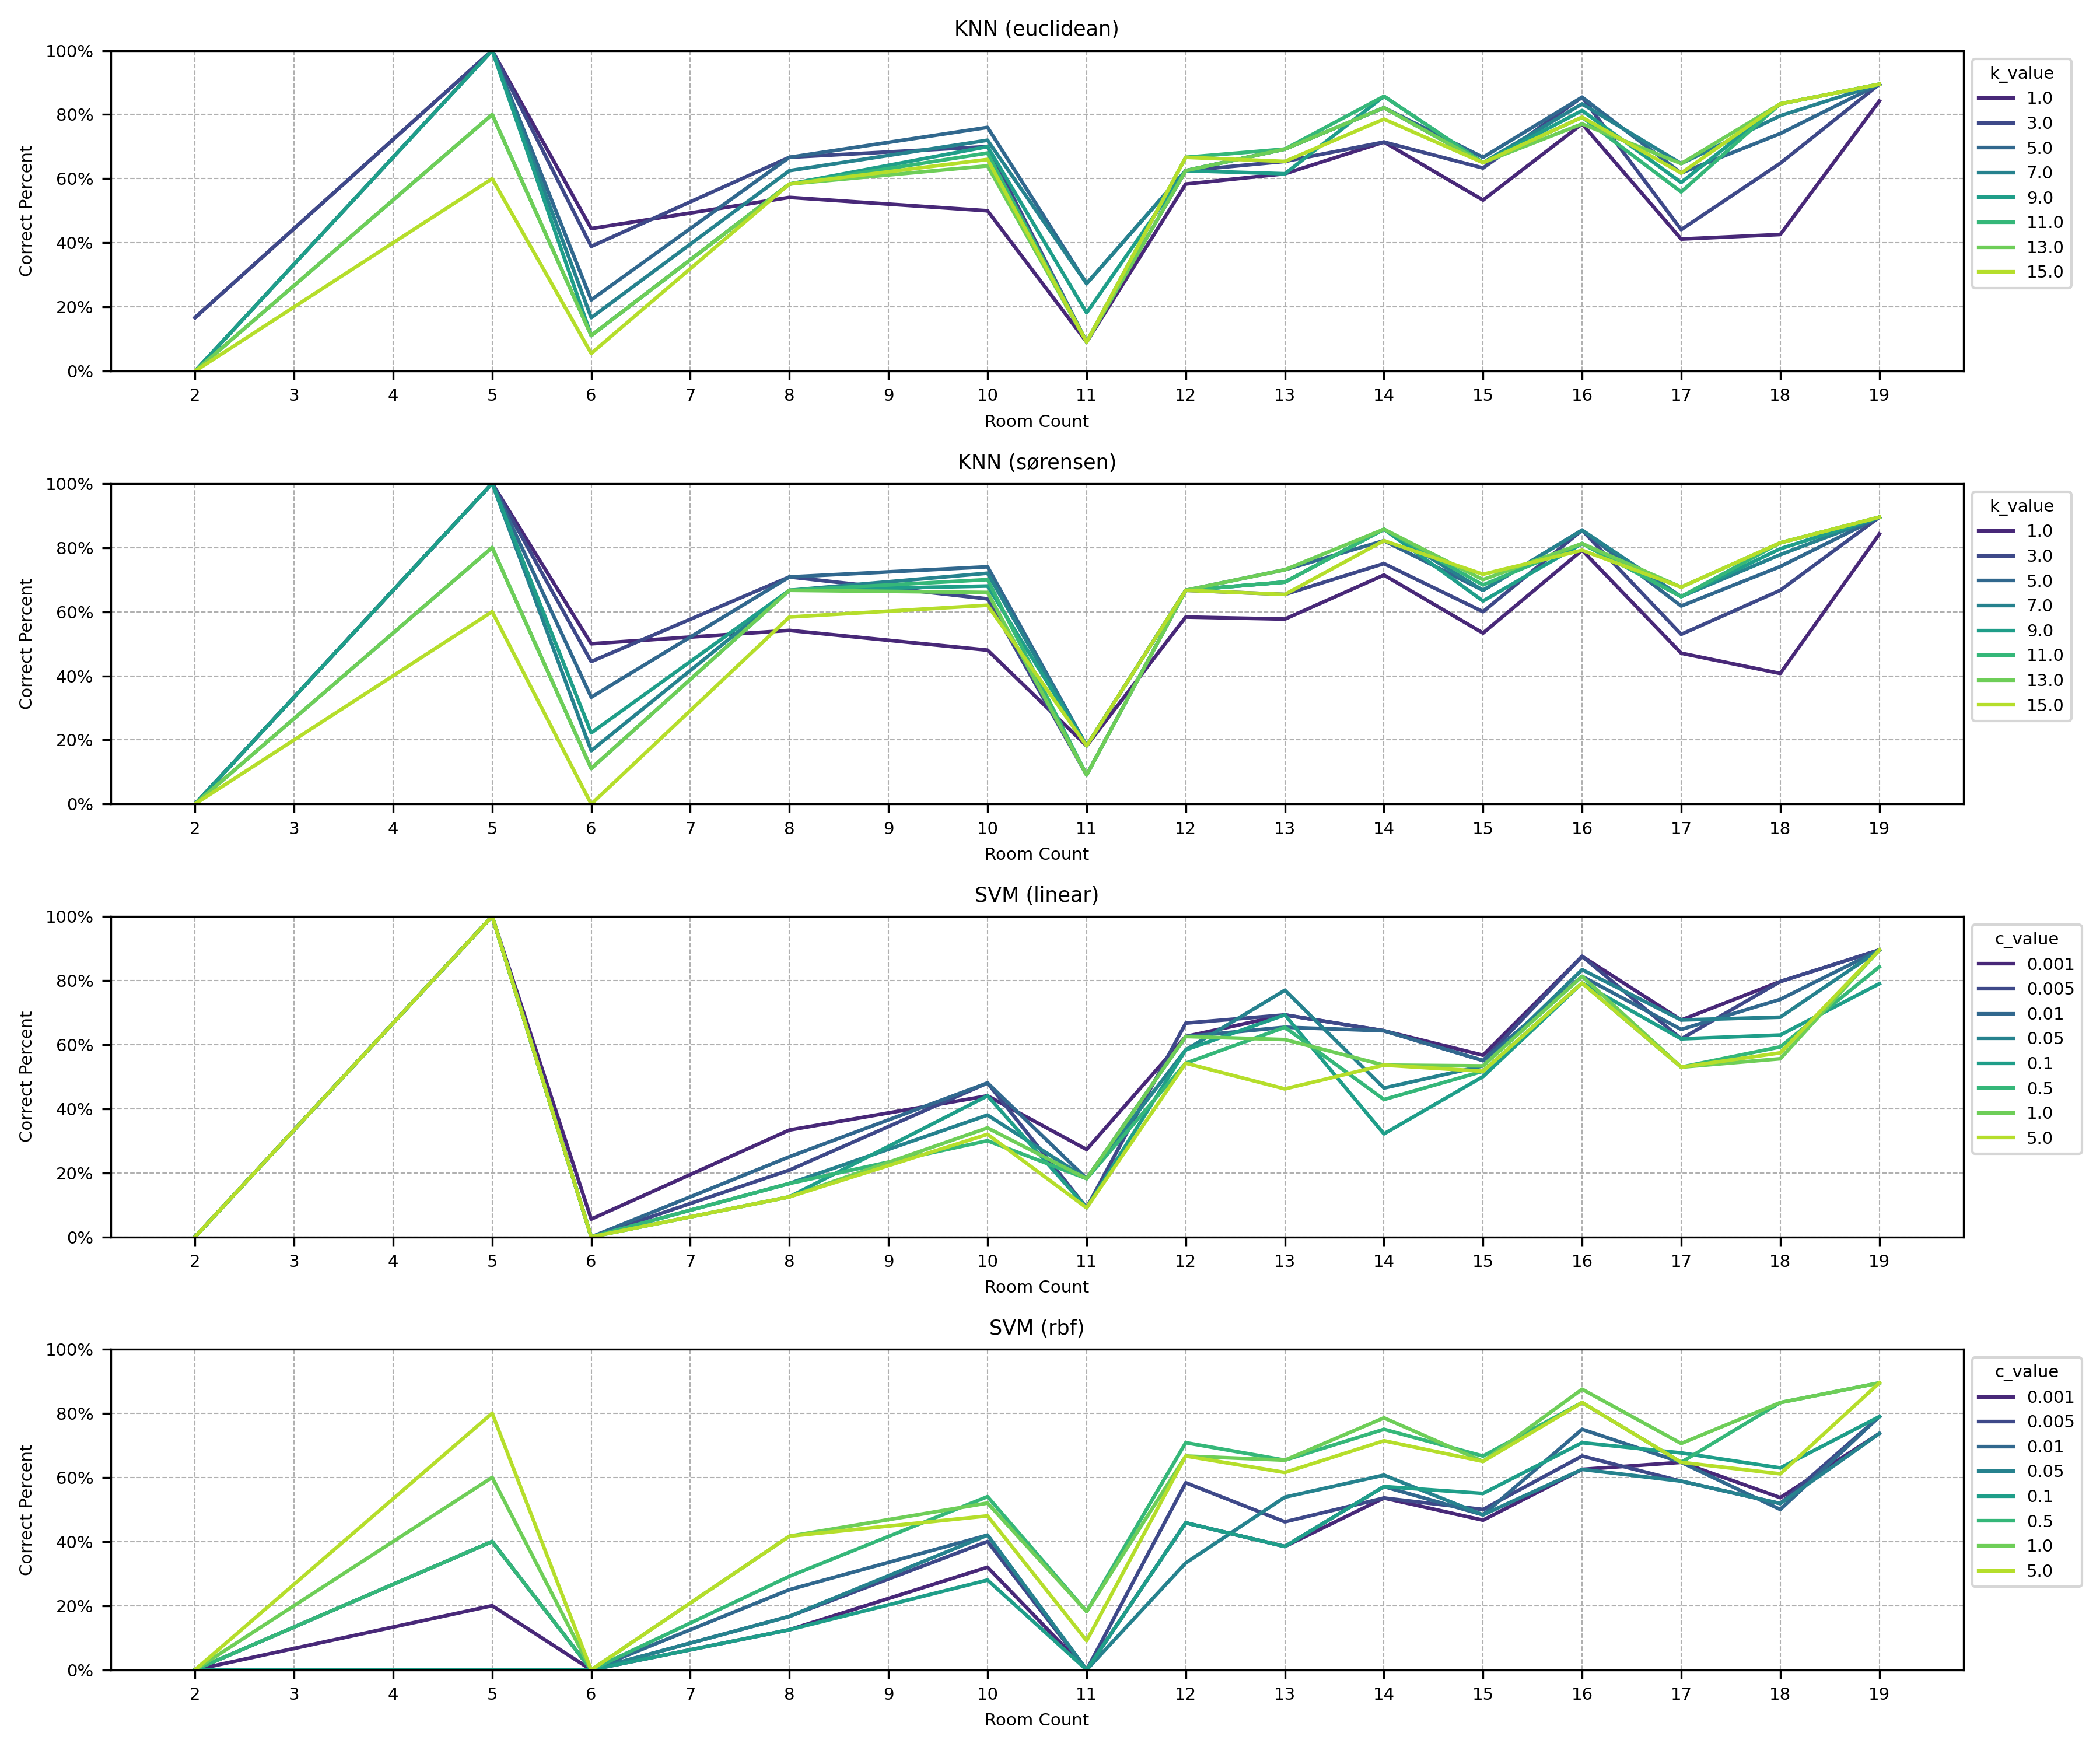
\includegraphics[width=0.8\textwidth]{images/05_best_parameters_all_01.png}
    \caption{Vergleich der Parameter in Abhängigkeit der Anzahl der Messungen}
    \label{fig:05_best_parameters_all_01}
\end{figure}

\begin{figure}[H]
    \centering
    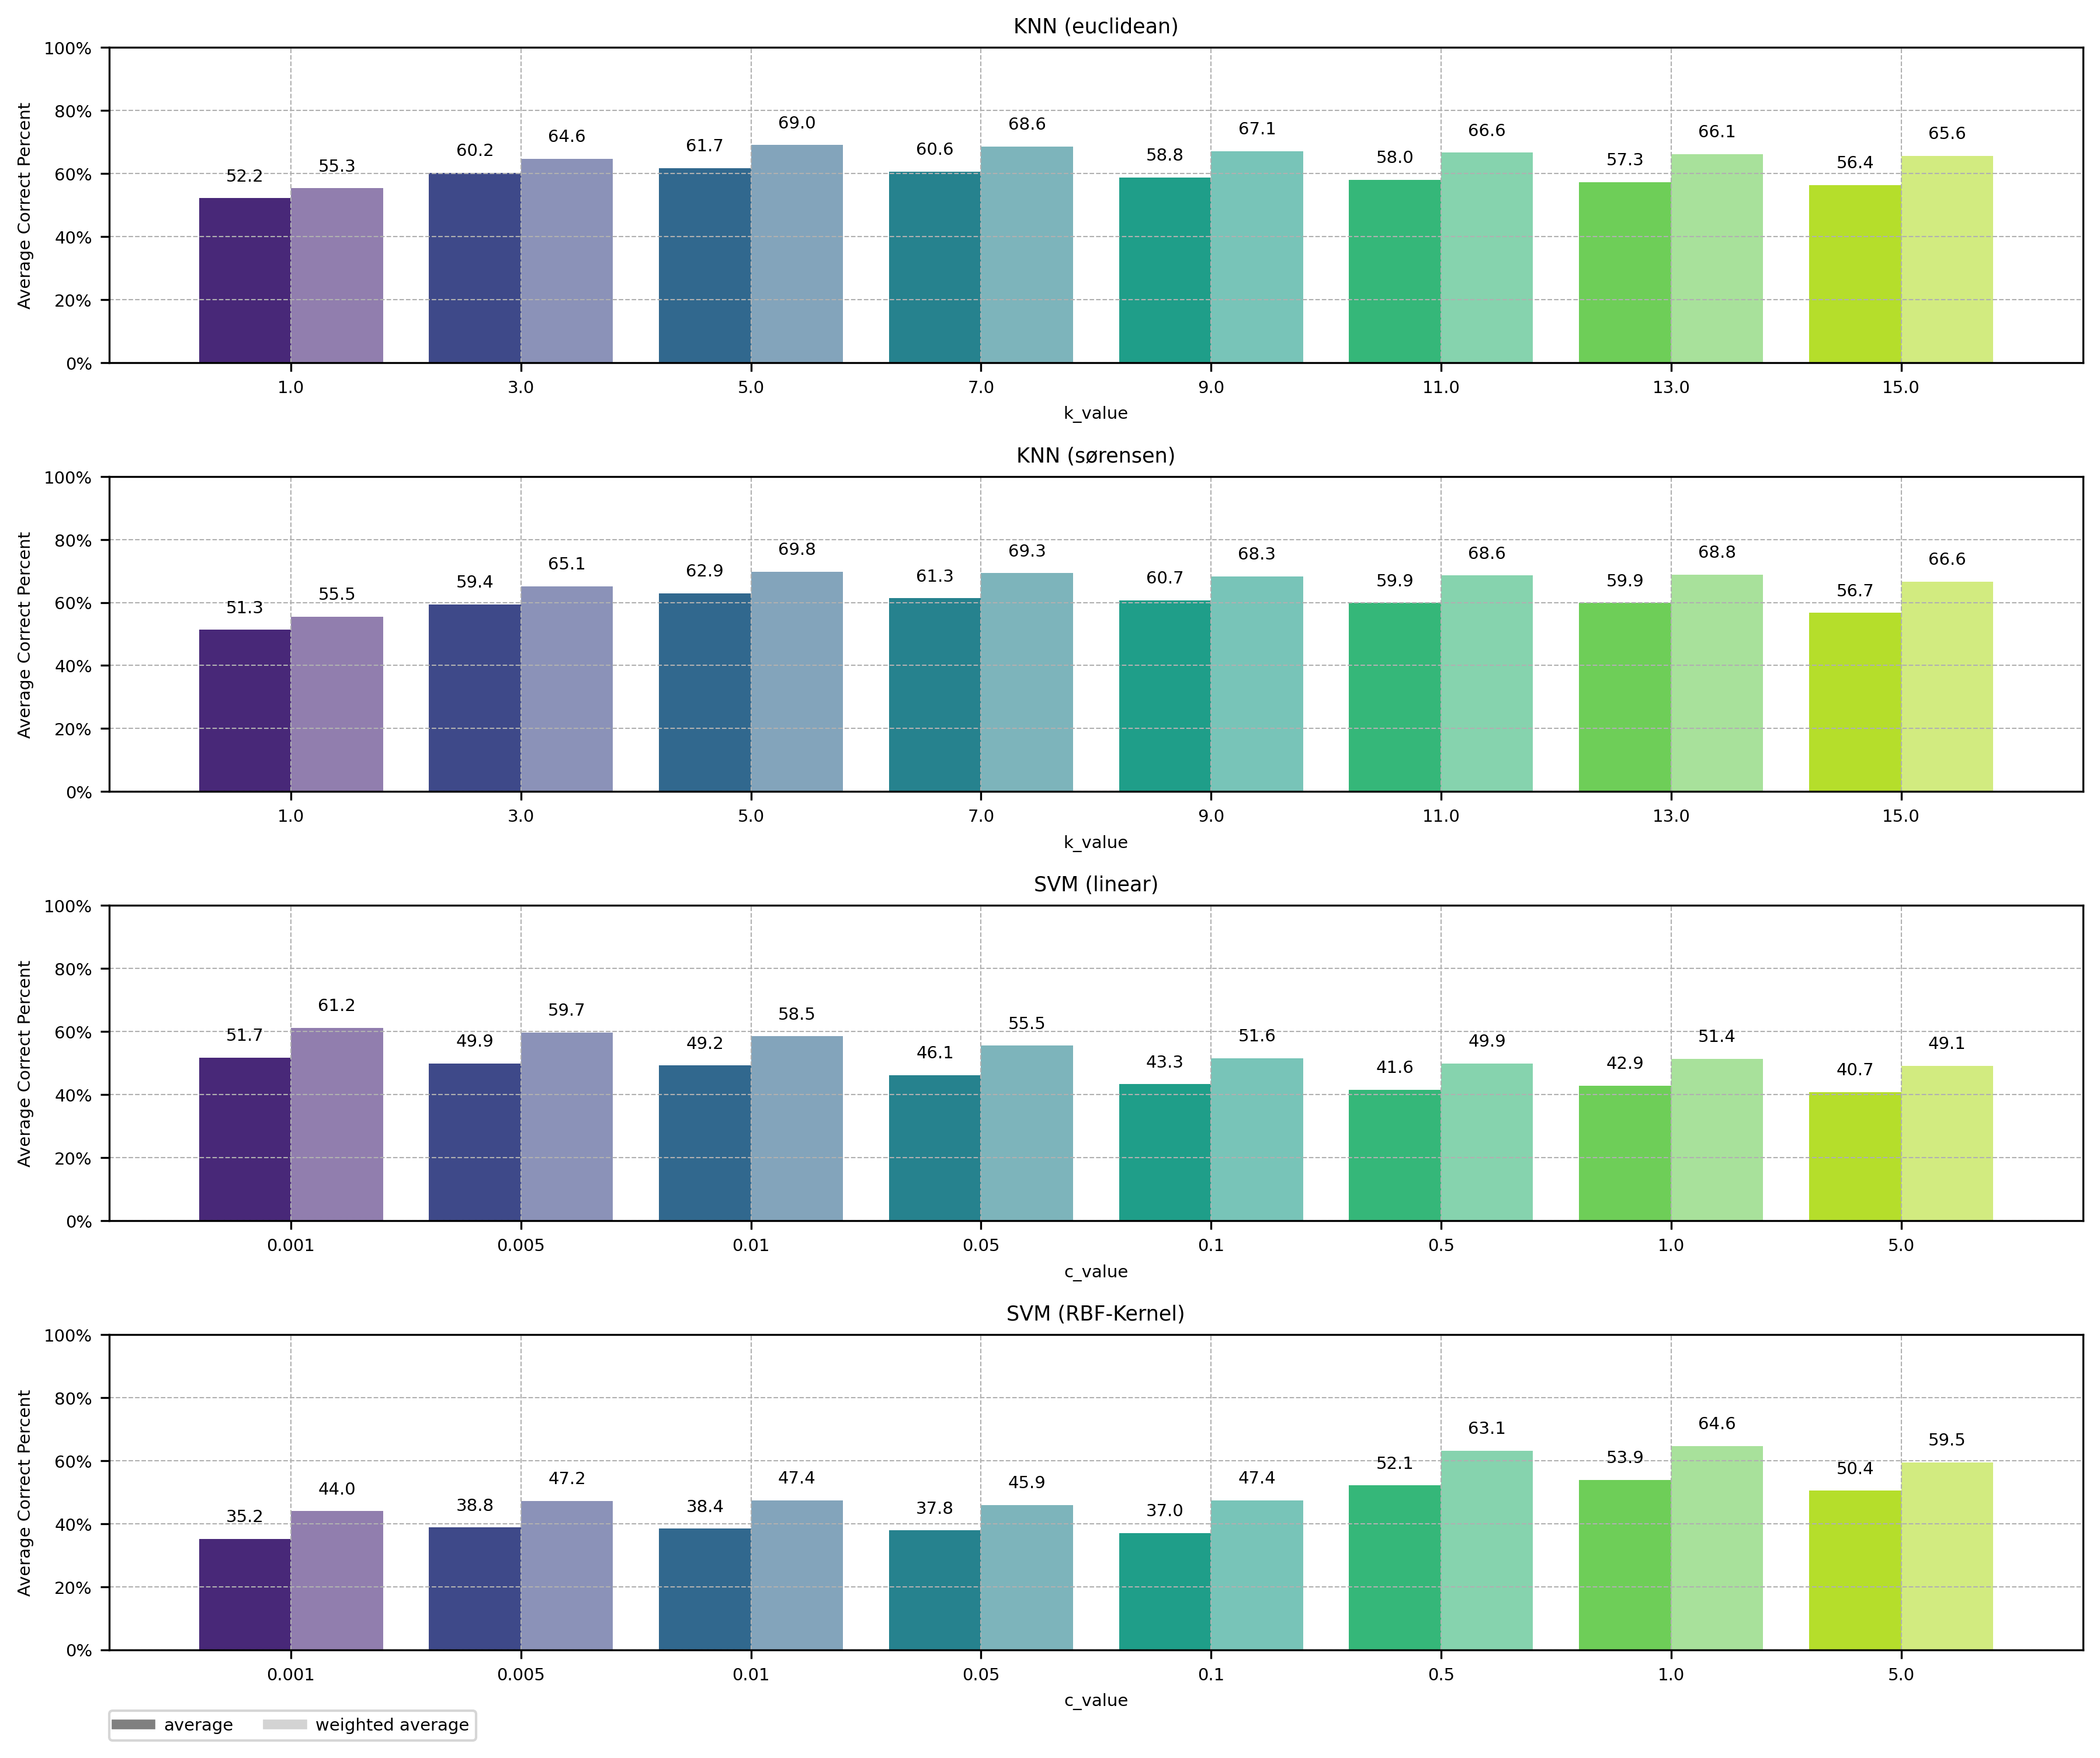
\includegraphics[width=0.8\textwidth]{images/05_best_parameters_all_03.png}
    \caption{Vergleich der durschnittlichen Genauigkeit der Parameter in Abhängigkeit der Anzahl der Messungen}
    \label{fig:05_best_parameters_all_03}
\end{figure}

% NICHT LÖSCHEN! WEIL QUELLE...
% Warum diese Parameter?
% \begin{itemize}
%     \item KNN: 1, 3, 5, 7, 9, 11, 13, 15 -> Weil ungerade (siehe Quelle bei KNN), im Wertebereich der Anzahl an Messungen pro Raum
%     \item RF: 50, 100, 150, 200, 250, 300, 350, 400 Wurde gewählt, weil 407 Messpunkte existieren
%     \item SVM: 0.001, 0.005, 0.01, 0.05, 0.1, 0.5, 1, 5 -> Quelle: Supervised Learning-Based Indoor Positioning System Using WiFi Fingerprints Seite 62
% \end{itemize}

% Ergebnisse:

% \begin{itemize}
%     \item KNN: 5, 7, 9
%     \item RF: 100, 200, 300
%     \item SVM (RBF): 0.5, 1, 5
%     \item SVM (Linear): 0.001, 0.005, 0.01
% \end{itemize}

\paragraph{\gls{knn}}

Wie in Abbildung \ref{fig:05_best_parameters_all_01} zu sehen ist, erzielen kleinere Werte für \( k \) sowohl bei der euklidischen als auch bei der Sørensen-Distanzmetrik bessere Ergebnisse in Räumen mit weniger Messungen, während größere Werte für \( k \) hingegen bei Räumen mit mehr Messungen von Vorteil sind. Im Durchschnitt konnten die besten Ergebnisse bei \( k = 5 \), \( k = 7 \) und \( k = 9 \) erzielt werden. Daher wurden diese Werte für die weiteren Analysen ausgewählt.

\paragraph{\gls{svm} (linear)}

Abbildung \ref{fig:05_best_parameters_all_03} zeigt, dass die Genauigkeit des \gls{svm}-Algorithmus mit linearem Kernel mit zunehmendem Wert für \( C \) abnimmt, wobei die besten Ergebnisse bei \( C = 0{,}001 \) erzielt wurden. Diese Ergebnisse gelten sowohl für den gewichteten (61,2 \%) als auch für den ungewichteten Durchschnitt (51,7 \%). Die zweit- und drittbesten Ergebnisse wurden für \( C = 0{,}005 \) und \( C = 0{,}01 \) erzielt. Daher wurden für die weitere Analyse die Werte \( C = 0{,}001 \), \( C = 0{,}005 \) und \( C = 0{,}01 \) ausgewählt.

\paragraph{\gls{svm} (RBF)}

Für den \gls{svm} Algorithmus mit dem RBF-Kernel wurden die besten Ergebnisse bei \( C = 1{,}0 \) erzielt (64,6 \% für den gewichteten und 53,9 \% für den ungewichteten Durchschnitt). Die zweit- und drittbesten Ergebnisse wurden bei \( C = 0{,}5 \) und \( C = 5{,}0 \) erreicht. Daher wurden für die weitere Analyse die Werte \( C = 0{,}5 \), \( C = 1{,}0 \) und \( C = 5{,}0 \) ausgewählt.

\begin{figure}[H]
    \centering
    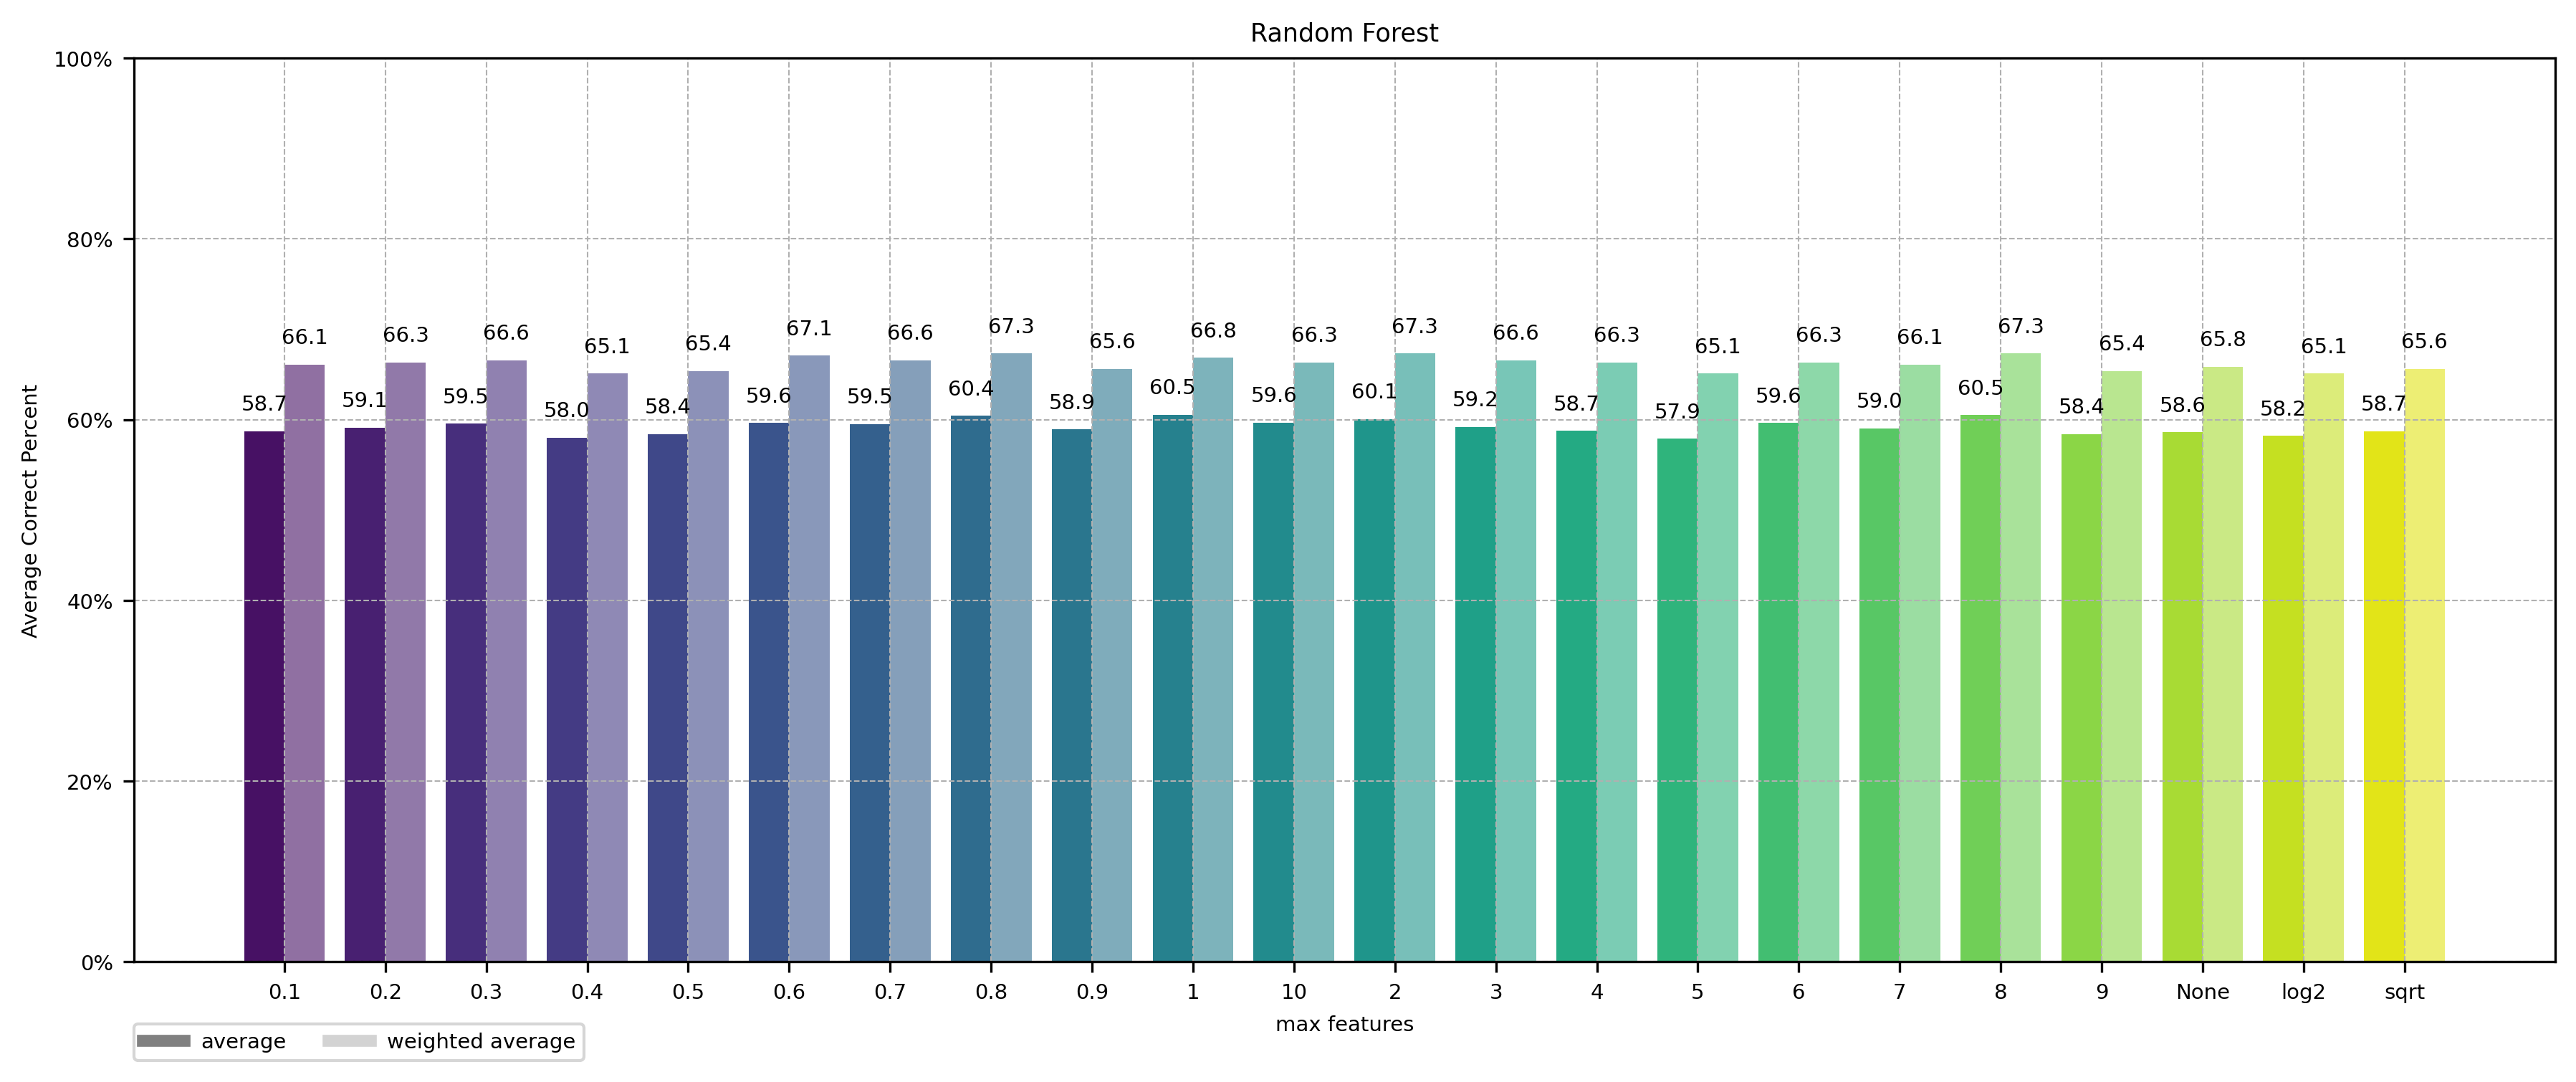
\includegraphics[width=0.8\textwidth]{images/05_best_parameters_random_forest_03.png}
    \caption{Vergleich der Parameter des Random Forest Algorithmus in Abhängigkeit der Anzahl der Messungen}
    \label{fig:05_best_parameters_random_forest_03}
\end{figure}

In Abbildung \ref{fig:05_best_parameters_random_forest_03} sind die durchschnittlichen Genauigkeiten der Parameter für den Random Forest Algorithmus dargestellt. Wie zu erkennen ist, hat die Wahl der Anzahl an Features keinen signifikanten Einfluss auf die Genauigkeit der Raumvorhersagen. Der Mittelwert gewichteten Durchschnitt liegt dabei bei 66,19 \% und bei den ungewichteten Durchschnitten bei 59,15 \%. Die besten Ergebnisse - auch wenn nur mit geringem Abstand - konnten für die Werte \texttt{max\_features = 0,8} (entspricht 80 \% der Features), \texttt{max\_features = 2} und \texttt{max\_features = 8} erzielt werden. Aus diesem Grund wurden für die weiteren Untersuchungen die Werte \texttt{max\_features = 0,8}, \texttt{max\_features = 2} und \texttt{max\_features = 8} ausgewählt.

\section{Untersuchungen des Einflusses verschiedener Datenaufbereitungsmethoden} \label{datenaufbereitung}

In dem folgenden Kapitel werden verschiedene Strategien zur Aufbereitung der Daten untersucht. Dafür wurde jede dieser Strategien in der API-Route \texttt{/measurements/predict} implementiert und kann über die Parameter dieses Endpunktes ausgewählt werden. Für die Analyse dieser Strategien wurde die in Kapitel \ref{testanwendung} vorgestellte Anwendung verwendet.

\subsubsection{Strategien zum Umgang mit fehlenden Werten} \label{strategien}

Im ersten Schritt der Datenaufbereitung wurde untersucht, wie sich verschiedene Strategien zum Umgang mit fehlenden Werten auf die Genauigkeit der Algorithmen auswirken.

Für die Erstellung der \gls{knn}-, \gls{svm}- und Random-Forest-Modelle wurden die Trainingsdaten in Form einer Matrix übergeben, in der für jeden Raum und jeden Router die RSSI-Werte aufgeführt sind. Da jedoch in der Realität nicht in jedem Raum dieselben Router empfangen werden und die Modelle nicht mit fehlenden Werten umgehen können, ist eine Aufbereitung dieser Daten erforderlich. Hierfür wurden verschiedene Strategien entwickelt:

\begin{enumerate}
    \item \textbf{Strategie -100:} Fehlenden Werten wird der Wert -100 dBm zugewiesen. Dieser Wert wurde gewählt, da das der kleinstmögliche RSSI-Wert ist (siehe Kapitel \ref{rssi}). Diese Strategie simuliert, dass der Router zwar erfasst wurde, aber nur ein sehr schwaches Signal gesendet hat.
    \item \textbf{Strategie use\_received:} Fehlende Werte werden durch den entsprechenden Wert in den Testdaten ersetzt. Diese Methode wurde gewählt, weil bei nicht vorhandenen Routern die Distanz null ist und diese somit beim \gls{knn}-Algorithmus ignoriert werden.
    \item \textbf{Strategie zero:} Fehlende Werte werden durch null ersetzt.
\end{enumerate}

In Abbildung \ref{fig:06_handle_missing_values_strategy_02} ist die Genauigkeit der Algorithmen in Abhängigkeit von der gewählten Strategie zum Umgang mit fehlenden Werten dargestellt. Es zeigt sich, dass die zweite Strategie bei \gls{knn} und Random Forest zu keiner Verbesserung der Ergebnisse führt und auch bei zunehmender Anzahl an Messungen keine Tendenz zu besseren Ergebnissen erkennbar ist. Auffällig bei diesen beiden Modellen ist, dass bei der \texttt{use\_received} Strategie eine leichte Steigerung der Genauigkeit bei 11 Messungen pro Raum zu beobachten ist, während die anderen beiden Strategien bei dieser Anzahl an Messungen eine entgegengesetzte Entwicklung zeigen. Die \texttt{use\_received} Strategie konnte bei 11 Messungen pro Raum zum Teil bessere Ergebnisse erzielen als die anderen beiden Strategien. Im direkten Vergleich der ersten und dritten Strategie für \gls{knn} und Random Forest ist zu erkennen, dass die Zuweisung von -100 dBm bei fehlenden Werten zu besseren Ergebnissen führt als die Ersetzung durch 0 dBm, auch wenn die Unterschiede gering sind.

Bei dem \gls{svm} Algorithmus zeigt sich im Gegensatz zu den anderen beiden Modellen, dass die Genauigkeit bei der zweiten Strategie mit zunehmender Anzahl an Messungen tendenziell steigt. Dennoch sind auch hier die anderen beiden Strategien überlegen.

\begin{figure}[H]
    \centering
    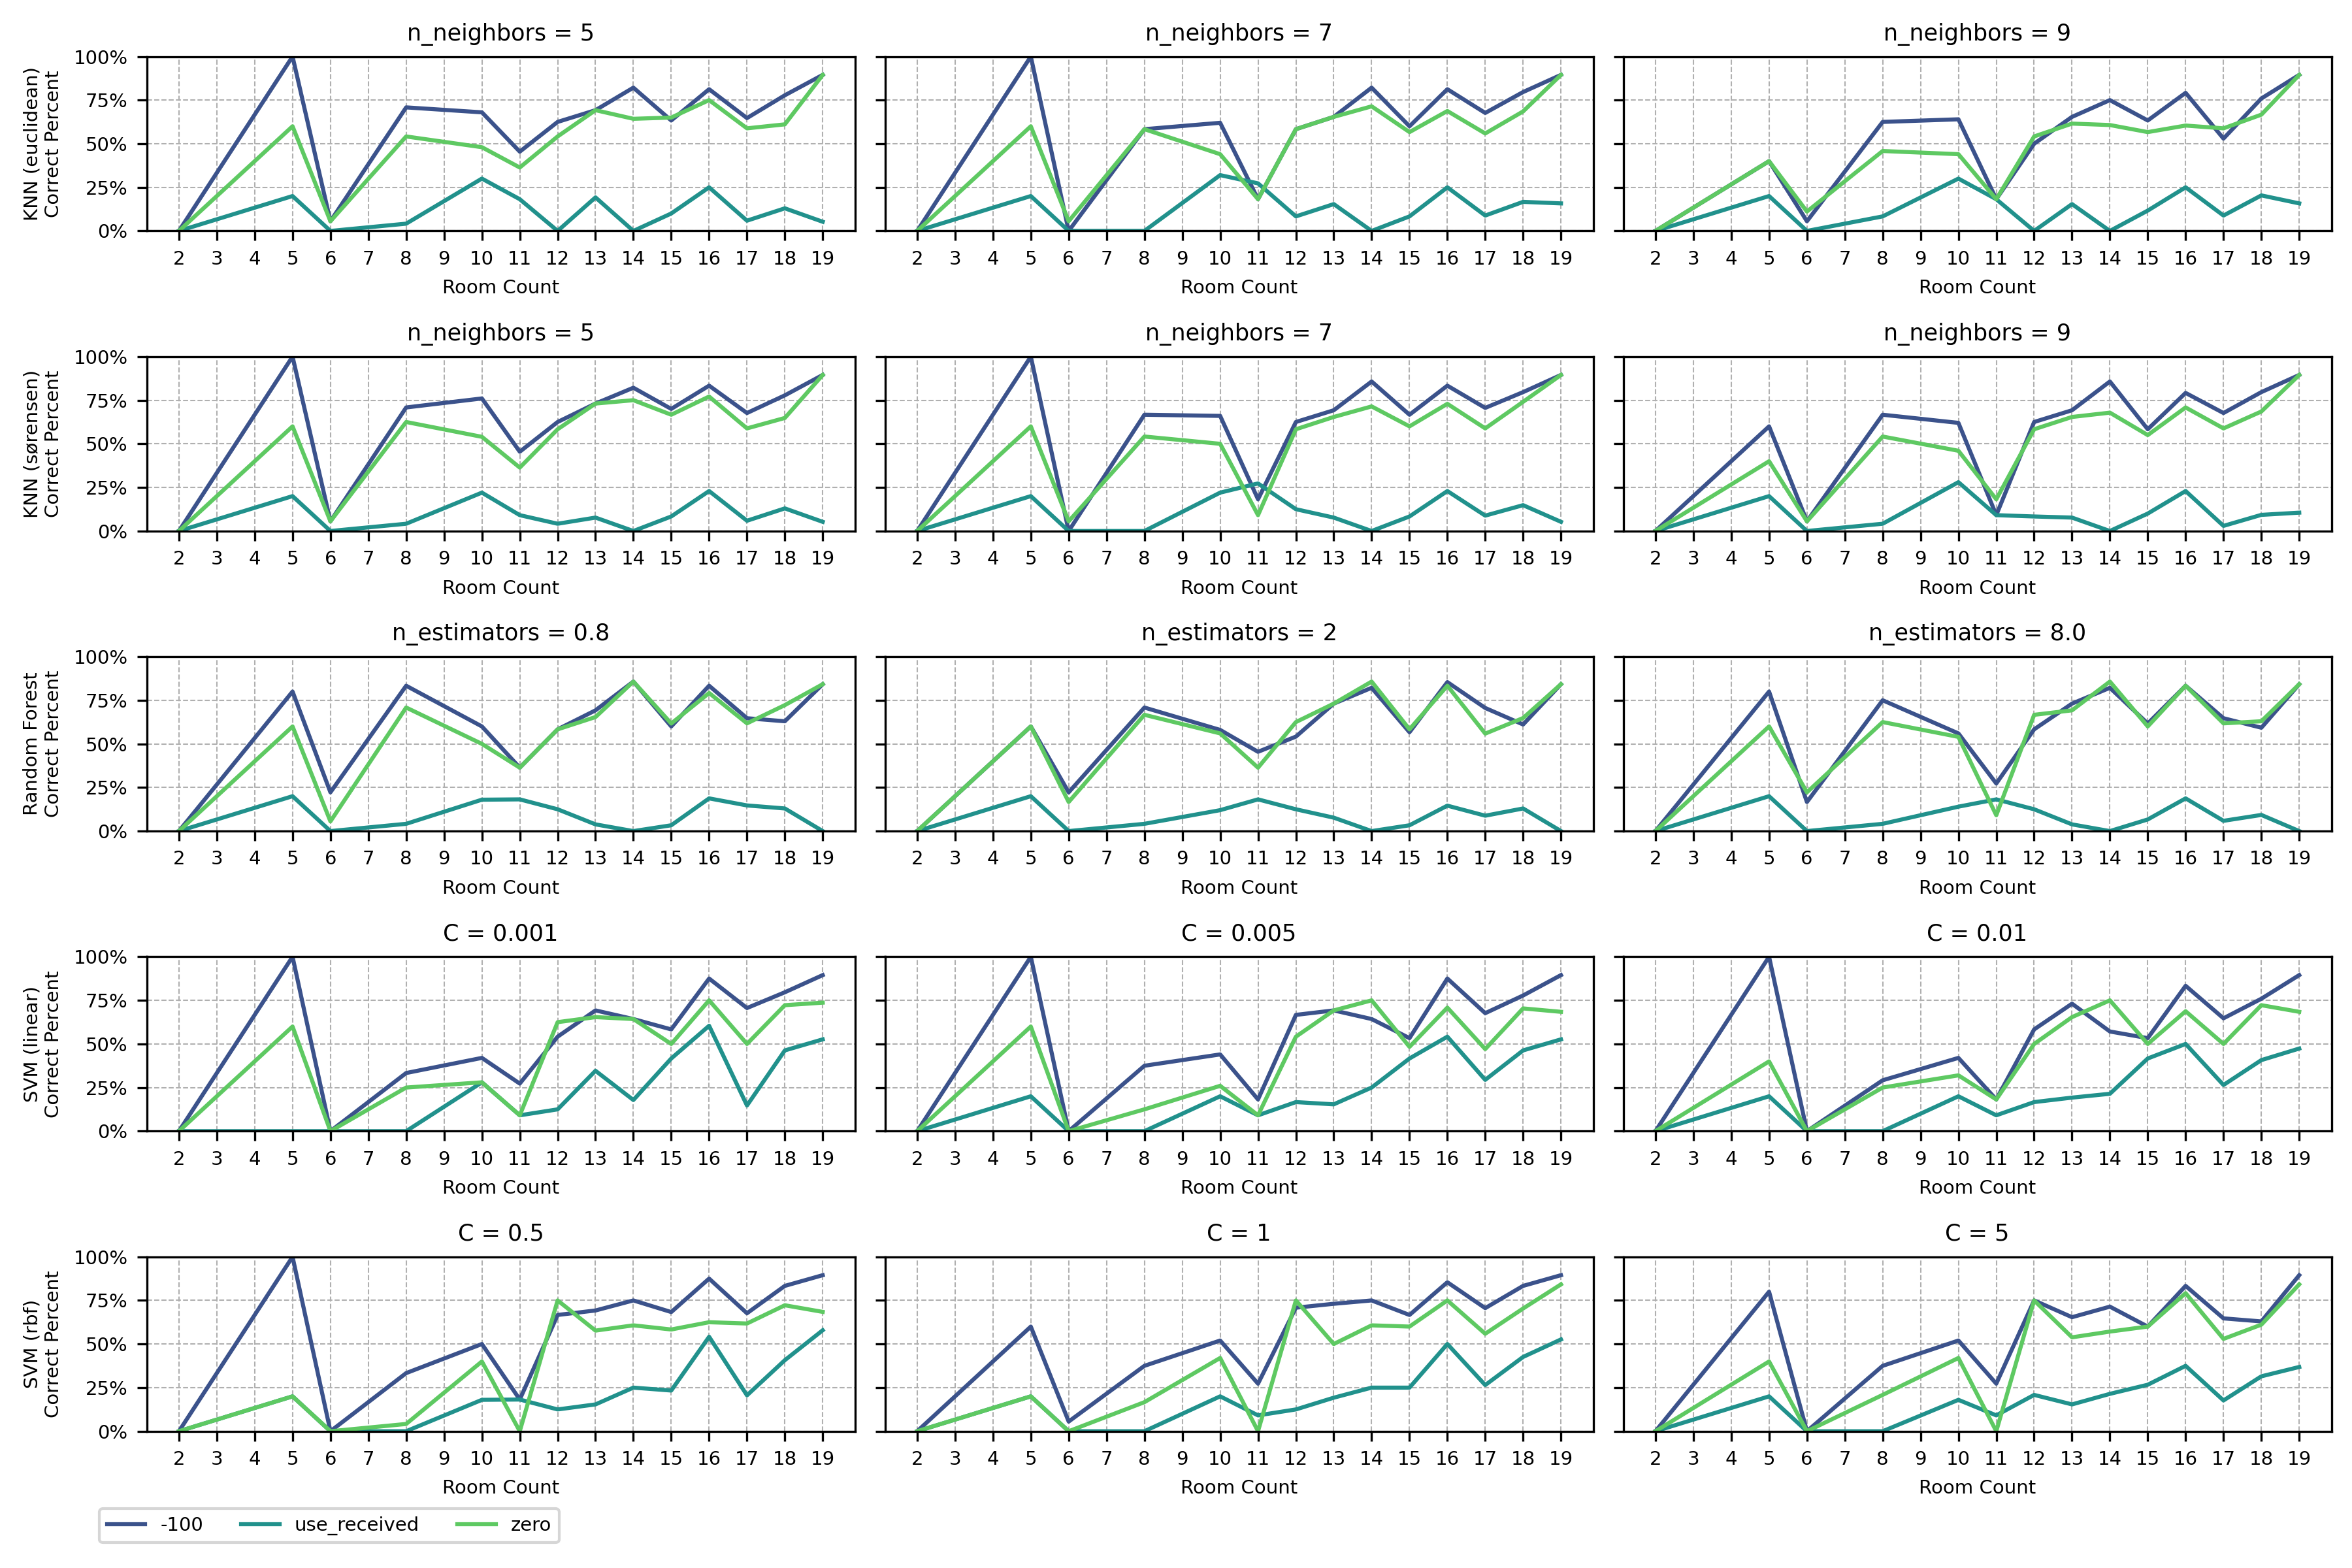
\includegraphics[width=0.8\textwidth]{images/06_handle_missing_values_strategy_02.png}
    \caption{Vergleich der Genauigkeit in Abhängigkeit der Strategie zum Umgang mit fehlenden Werten}
    \label{fig:06_handle_missing_values_strategy_02}
\end{figure}

Wie in Abbildung \ref{fig:06_handle_missing_values_strategy_03} zu erkennen ist, führt die erste Strategie in allen Fällen zu den besten Ergebnissen, wenn die durchschnittliche Genauigkeit betrachtet wird. Aus diesem Grund werden in den weiteren Untersuchungen fehlende Werte durch -100 dBm ersetzt.

\begin{figure}[H]
    \centering
    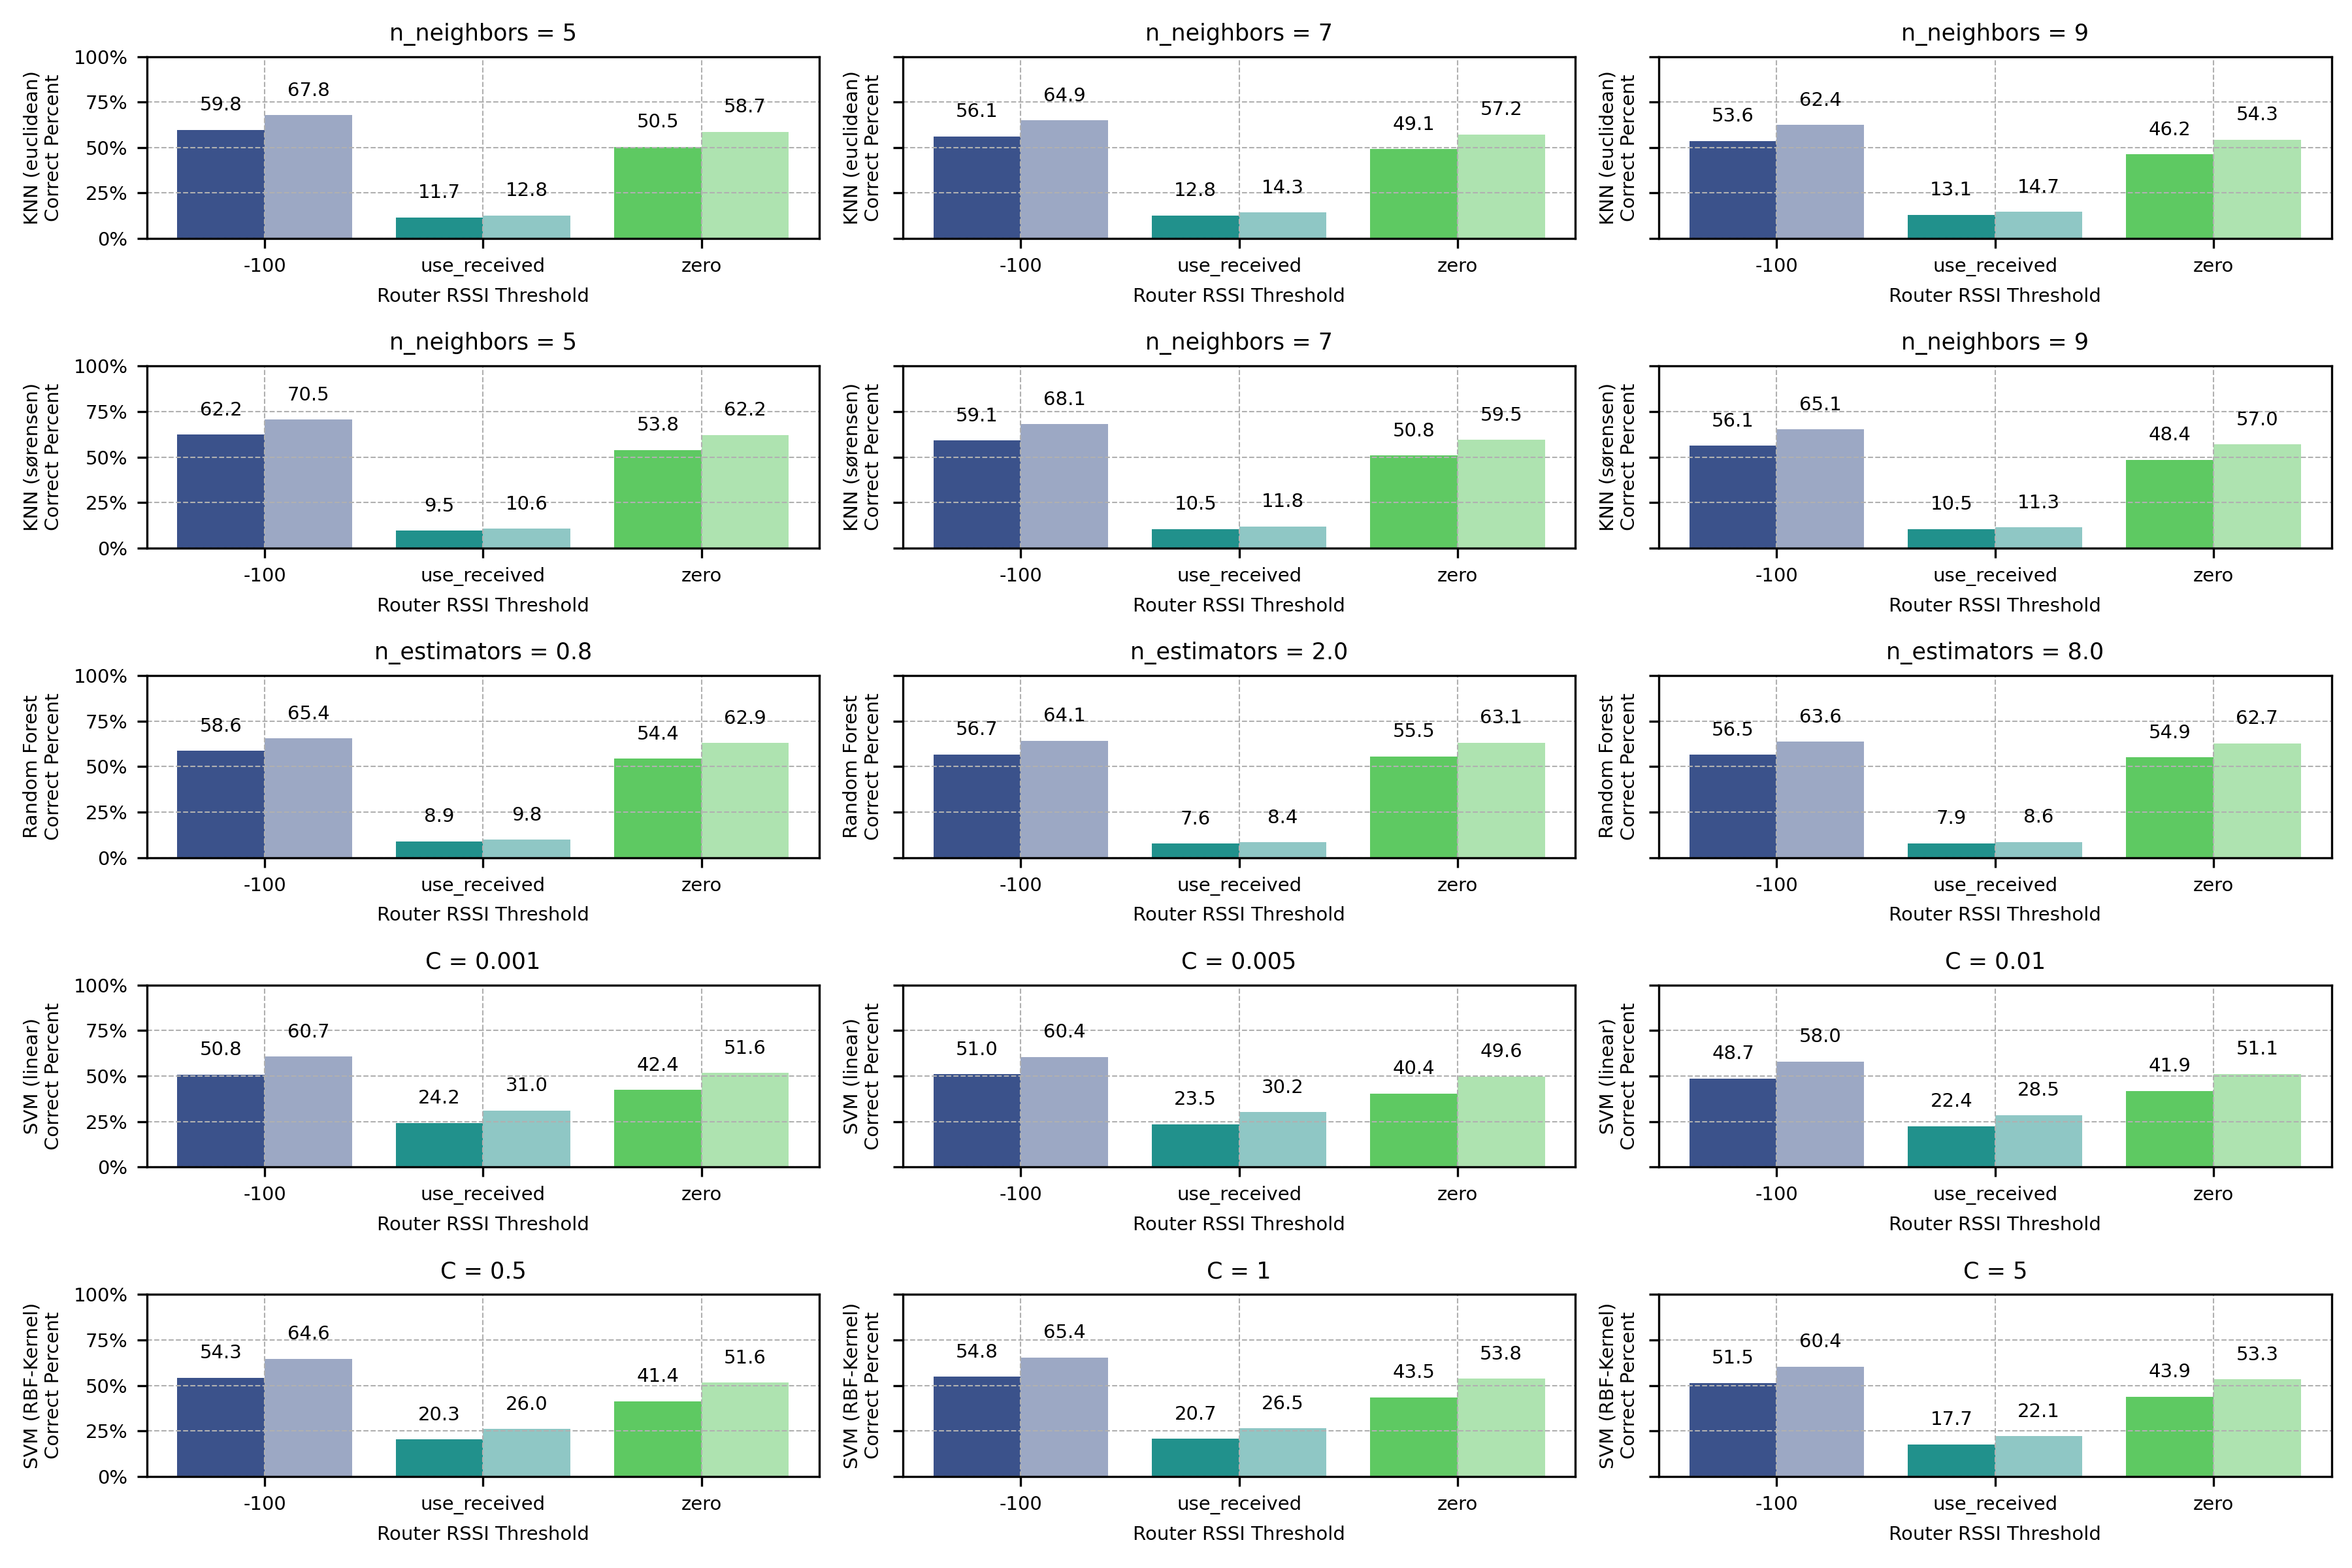
\includegraphics[width=0.8\textwidth]{images/06_handle_missing_values_strategy_03.png}
    \caption{Vergleich der durchschnittlichen Genauigkeit in Abhängigkeit der Strategie zum Umgang mit fehlenden Werten}
    \label{fig:06_handle_missing_values_strategy_03}
\end{figure}

\subsubsection{Einfluss der verwendeten Router}

Im zweiten Schritt der Datenaufbereitung wird untersucht, ob die Auswahl der Router einen Einfluss auf die Genauigkeit der Modelle hat. Der Gedanke hinter diesem Aufbereitungsschritt ist, dass nicht alle empfangenen Access Points ortsgebunden sind (z. B. Hotspots von mobilen Endgeräten) und somit einen negativen Einfluss auf die korrekte Raumvorhersage haben können. Deswegen könnte es von Vorteil sein, wenn nur die Access Points der eduroam-Infrastruktur (\textit{eduroam}, \textit{HowToUseEduroam} und \textit{Gast@HTW}) für die Vorhersagen verwendet werden.

Aus diesem Grund wird in diesem Aufbereitungsschritt untersucht, wie sich die Genauigkeit der Modelle verhält, wenn nur die Router der \textit{eduroam}-Infrastruktur für die Vorhersagen verwendet werden.

Wie in Abbildung \ref{fig:07_router_selection_02} zu erkennen ist, sind die Ergebnisse für alle Modelle und alle Parameterkonfigurationen - mit Ausnahme von den Ergebnissen bei 5 Messungen pro Raum - fast identisch. Dies deutet darauf hin, dass die Auswahl der Router bei diesen Daten keinen signifikanten Einfluss auf die Genauigkeit der Modelle hat und dass in dem Raum in dem 5 Messungen durchgeführt wurden die nicht-\textit{eduroam} Access Points einen besonders großen Einfluss haben bzw. die \textit{eduroam} Access-Points nicht aussagekräftig genug sind. Für die weiteren Untersuchungen wurde sich daher dafür entschieden nur die \textit{eduroam} Router zu betrachten, da bei diesen Routern davon ausgegangen werden kann, dass diese ihre Position nicht verändern und die Unterschiede - abgesehen von dem Raum mit 5 Messungen - minimal sind.

\begin{figure}[H]
    \centering
    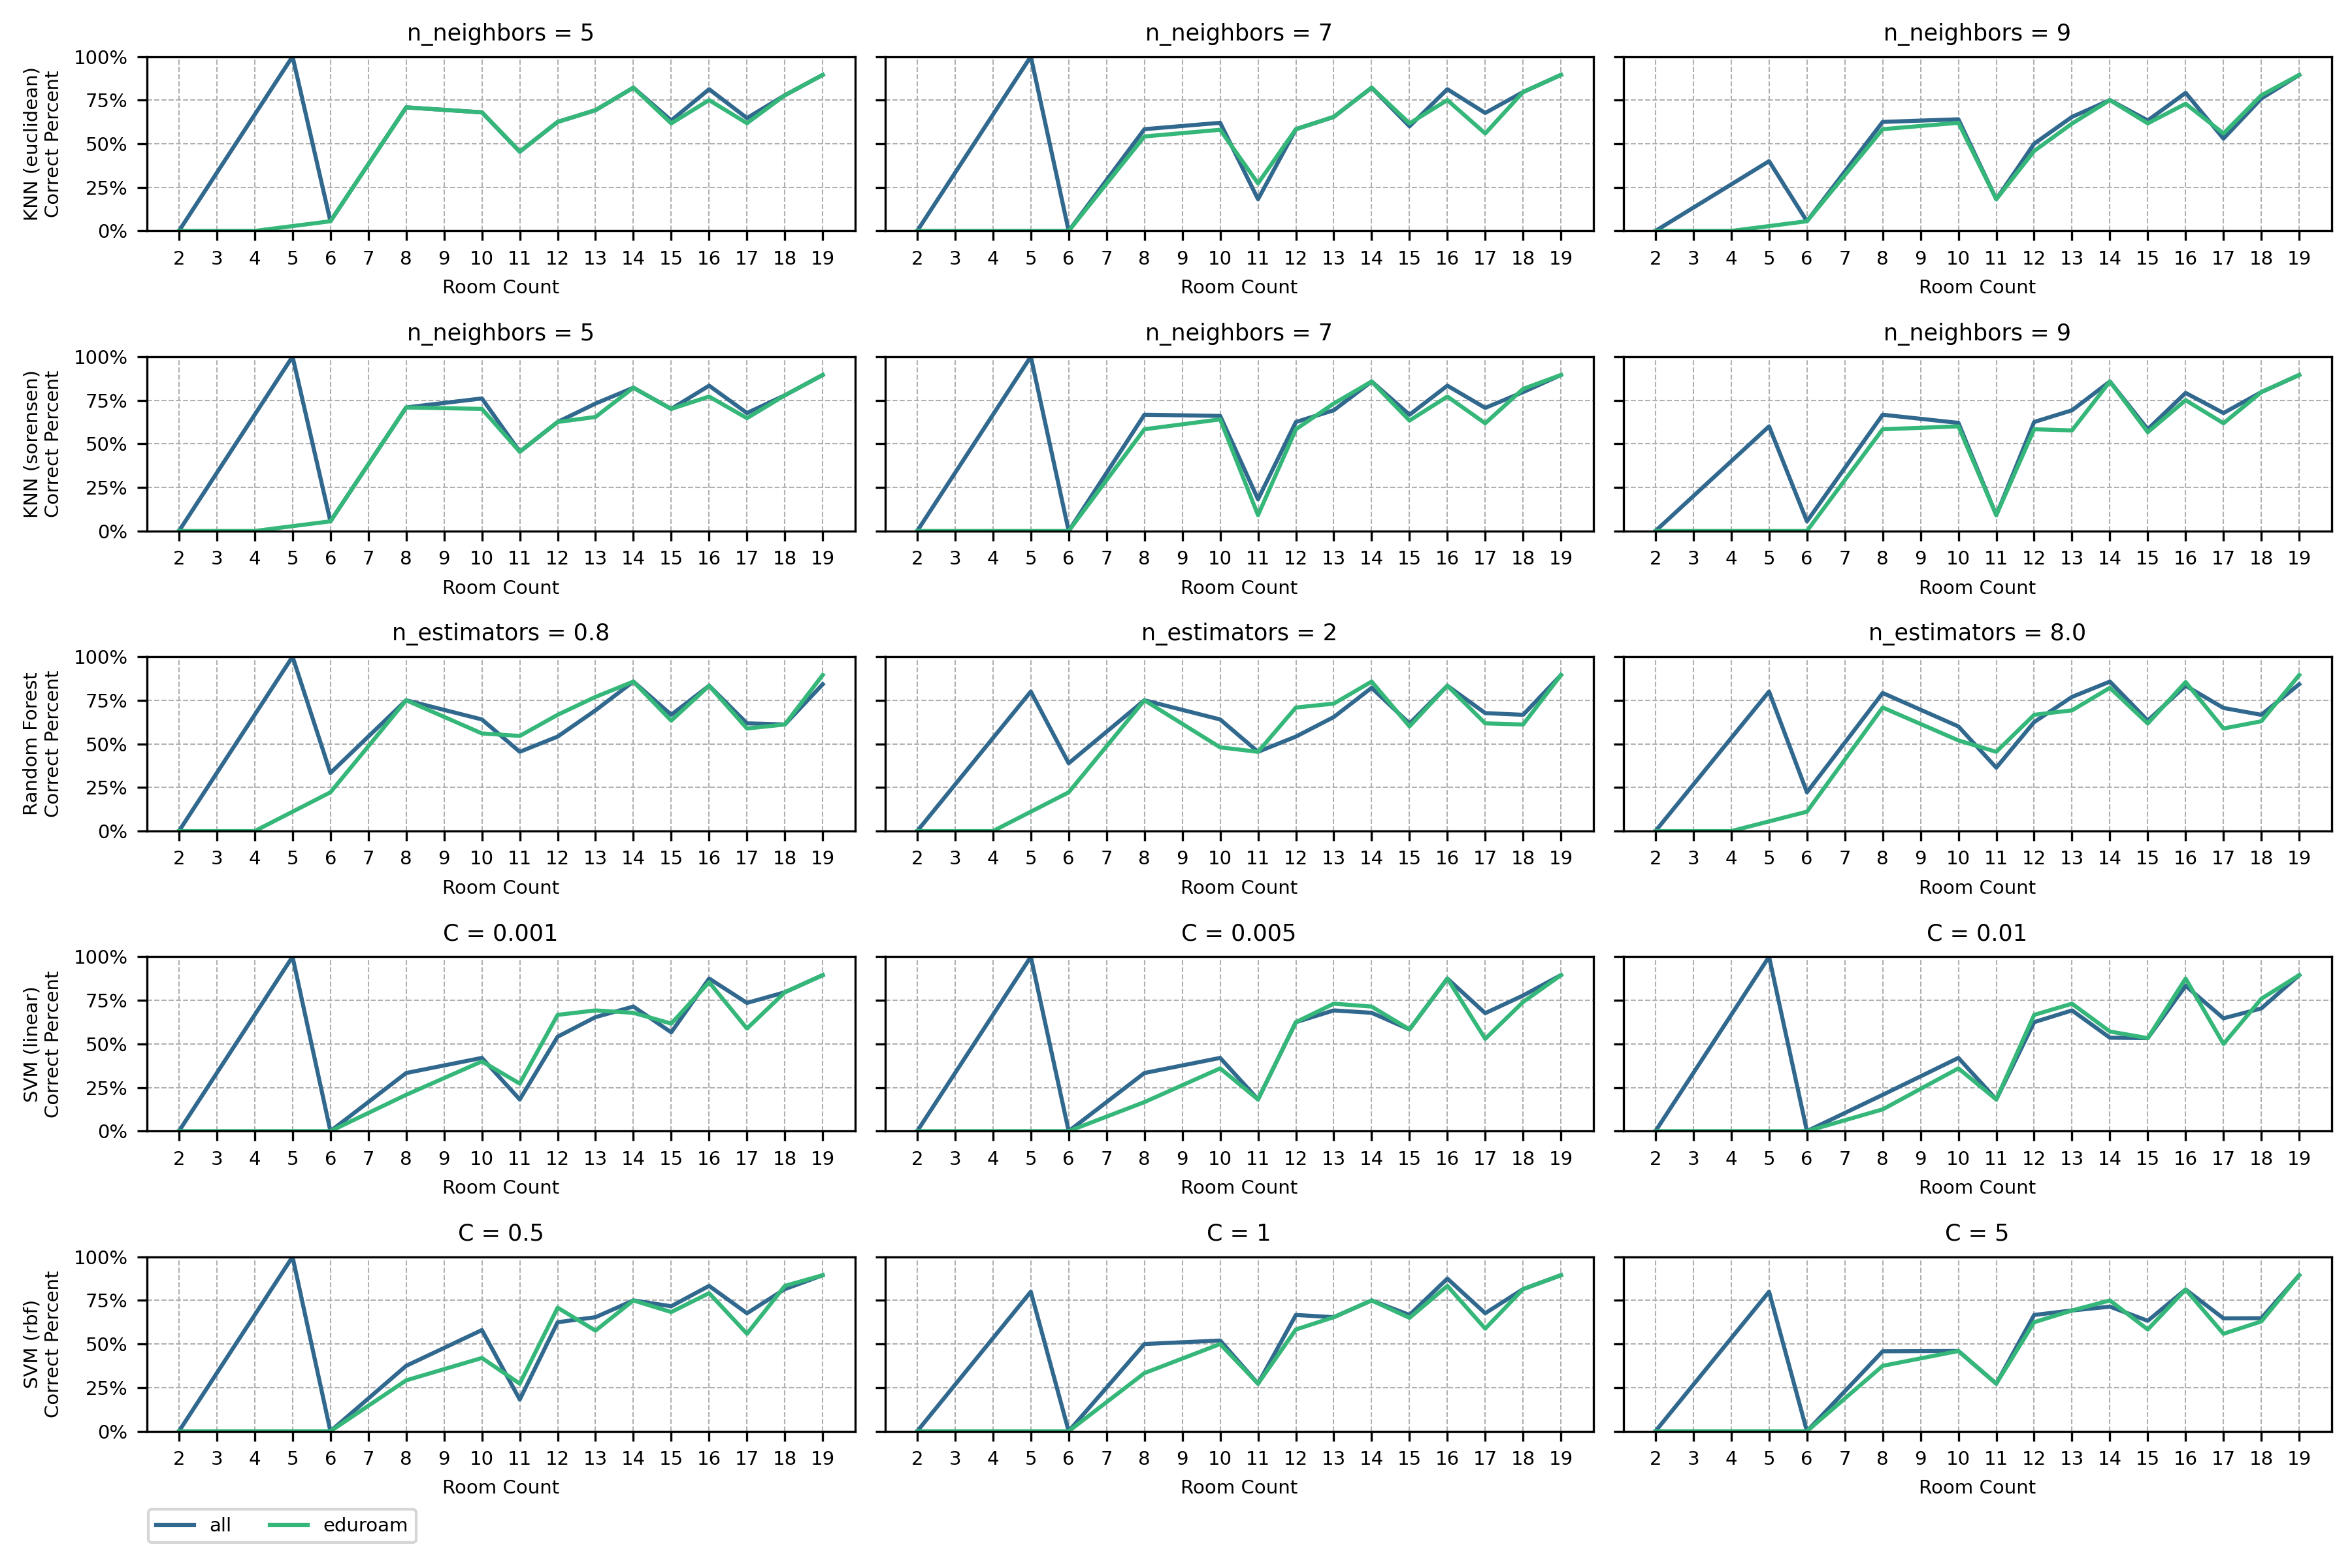
\includegraphics[width=0.8\textwidth]{images/07_router_selection_02.png}
    \caption{Vergleich der Genauigkeit in Abhängigkeit der Strategie zur Auswahl der Router}
    \label{fig:07_router_selection_02}
\end{figure}

\subsubsection{Filterung von RSSI-Werten}
\subsubsection{Berücksichtigung nur häufig auftretender Router}

Im dritten Schritt der Datenaufbereitung wird analysiert, ob die Genauigkeit verbessert werden kann, wenn nur Access Points berücksichtigt werden, die in mehreren Messungen eines Raums erfasst wurden. Die zugrunde liegende Annahme ist, dass Router, die häufiger in einem Raum empfangen werden, repräsentativer sind als solche, die nur selten erfasst werden. Aus diesem Grund wurden verschiedene Schwellenwerte getestet, die den Prozentsatz der berücksichtigten Router angeben. Dabei wurde unter anderem die bisherige Einstellung, bei der alle Router einbezogen werden, sowie die Schwellenwerte von 25 \%, 50 \% und 75 \% untersucht. Das bedeutet, dass beispielsweise nur die Router berücksichtigt werden, die in mindestens 25 \% der Messungen eines Raums vorhanden sind.

\begin{figure}[H]
    \centering
    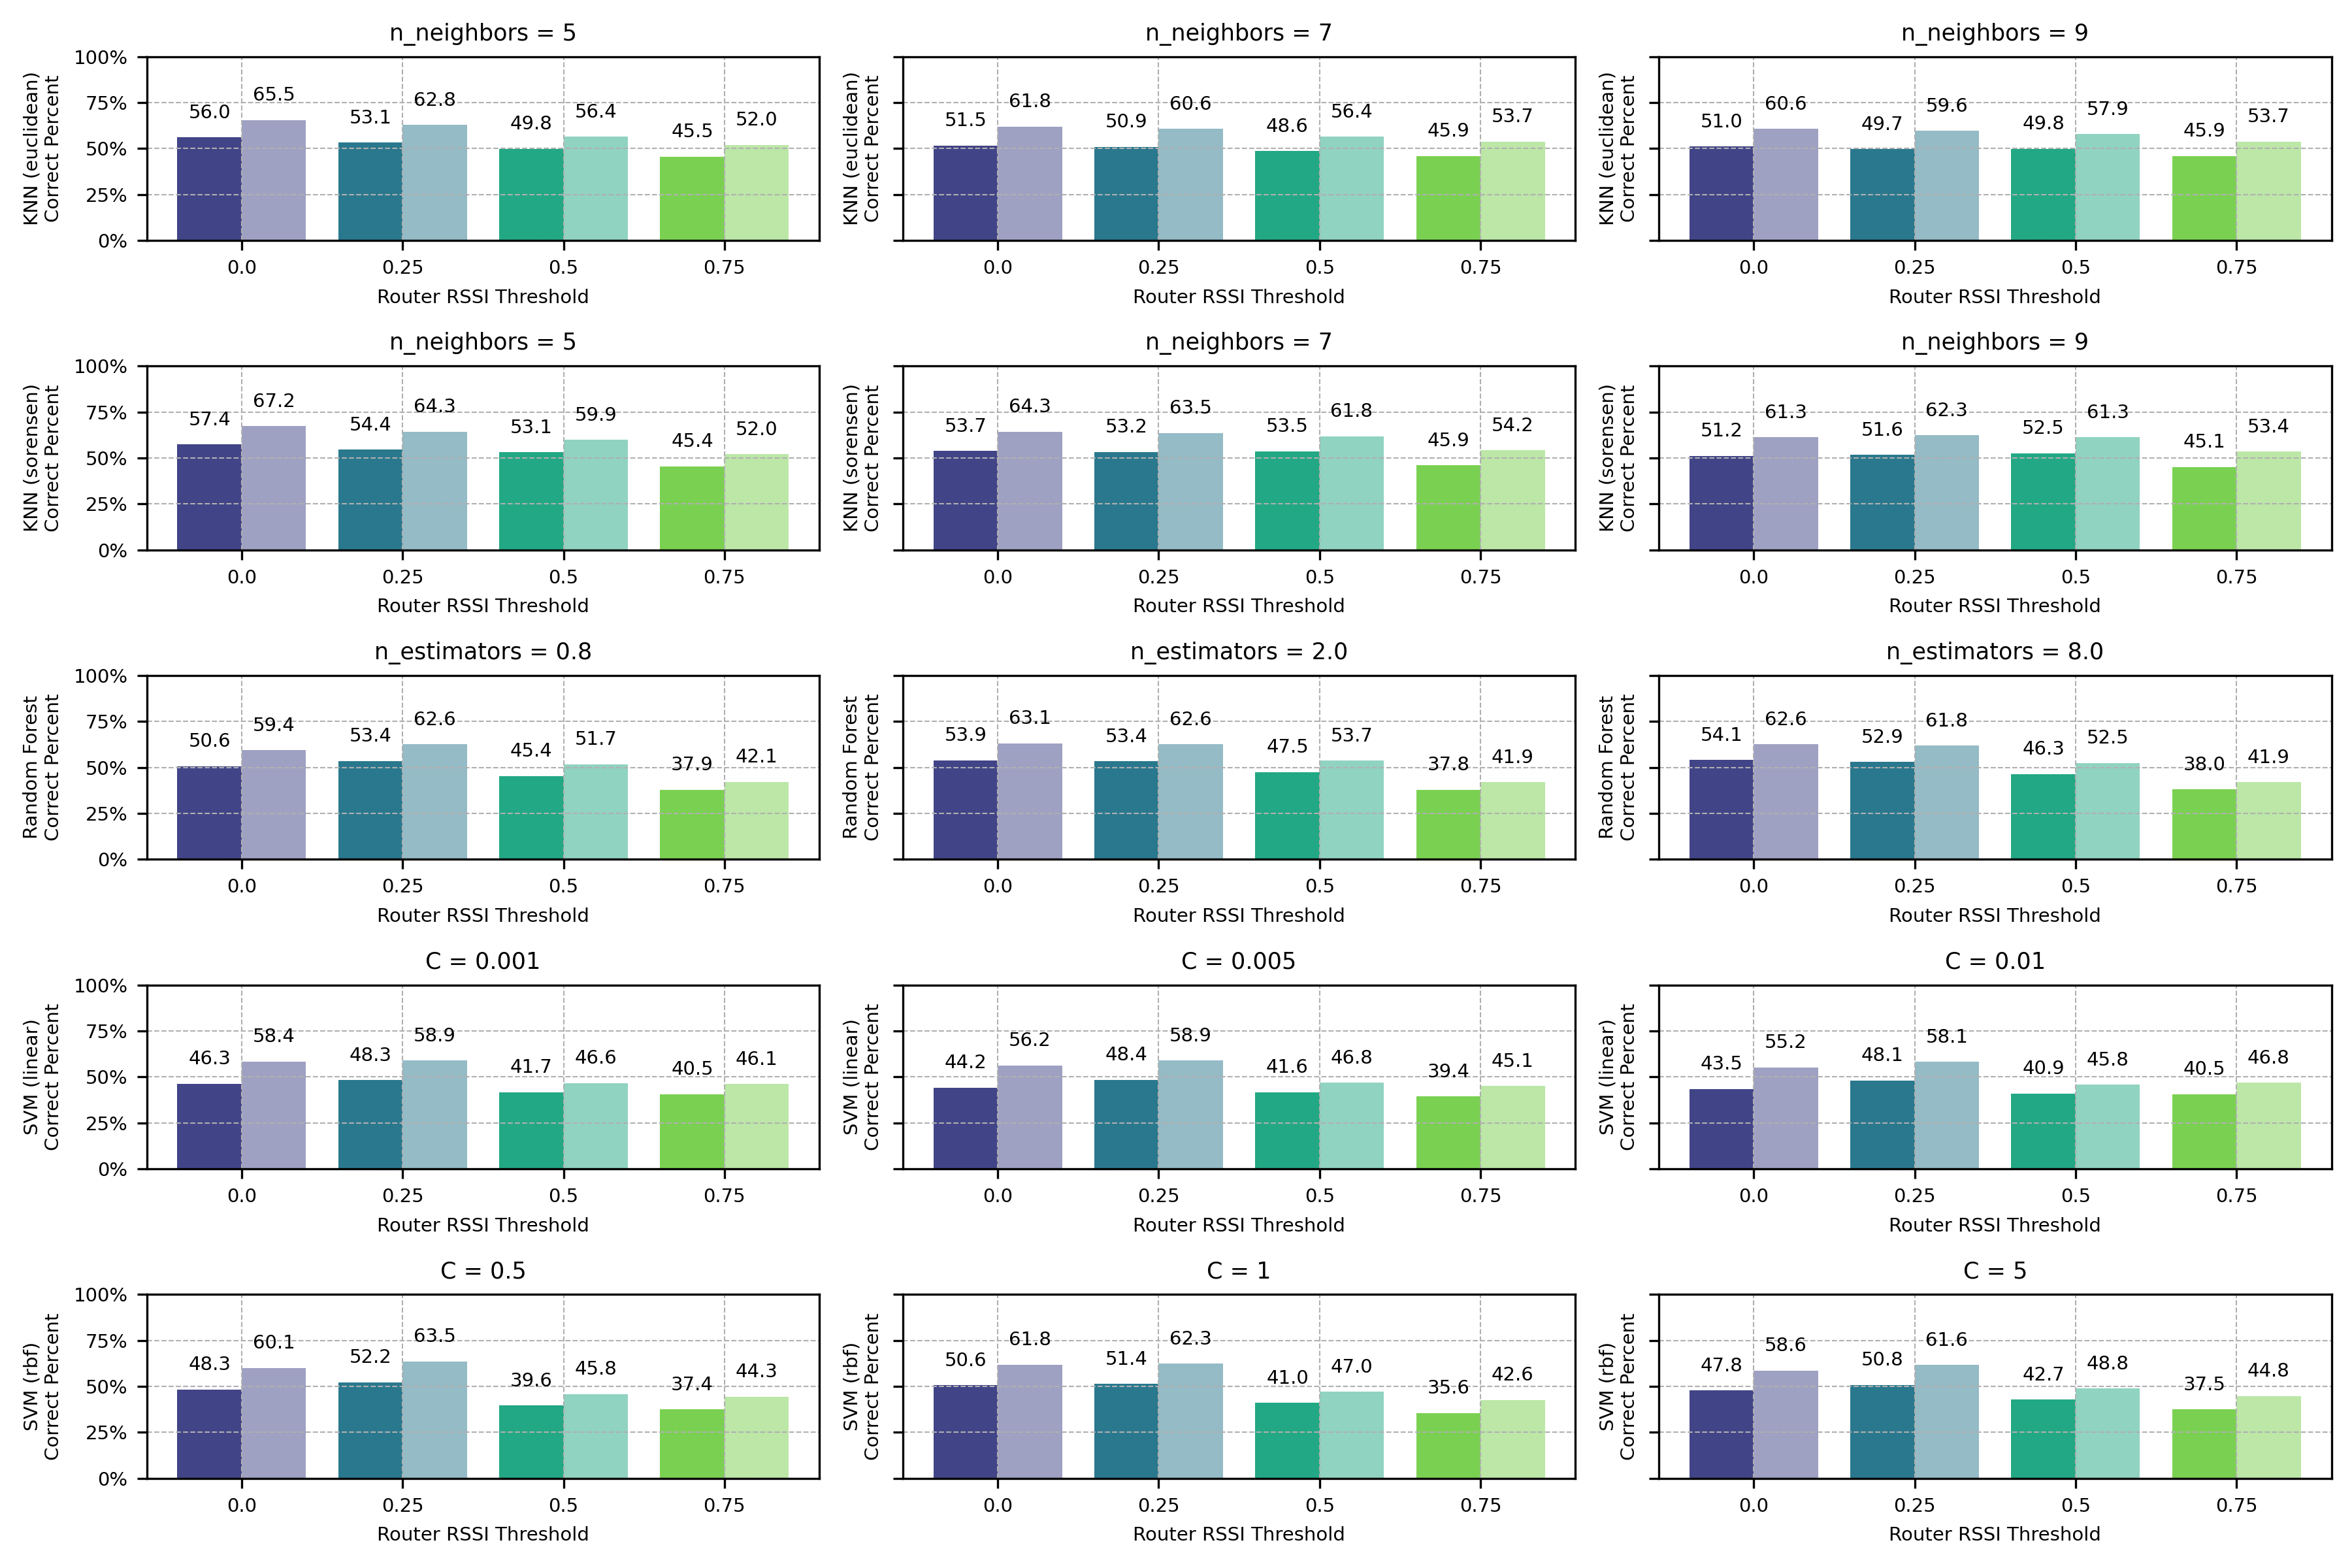
\includegraphics[width=0.8\textwidth]{images/08_router_presence_threshold_03.png}
    \caption{Vergleich der durchschnittlichen Genauigkeit in Abhängigkeit des Schwellenwerts für die Anzahl der Messungen eines Routers}
    \label{fig:08_router_presence_threshold_03}
\end{figure}

Wie in Abbildung \ref{fig:08_router_presence_threshold_03} zu sehen ist, sinkt die Genauigkeit bei beiden \gls{knn}-Modellen, mit Ausnahme der Sørensen Distanzmetrik für den Wert k = 9, sowie bei dem Random Forest Modell, mit Ausnahme der Werte für \texttt{max\_features = 0,8}, mit steigendem Schwellenwert. Bei dem \gls{knn} Algorithmus unter Verwendung der Sørensen Distanz und k = 9 und dem Random Forest Algorithmus mit \texttt{max\_features = 0,8} zeigt der Schwellenwert von 25 \% jedoch eine etwas bessere Genauigkeit als der Schwellenwert von 0 \%. Bei dem \gls{svm} Modell zeigt sich unabhängig vom Kernel, dass die Ergebnisse bei einem Schwellenwert von 25 \% bei allen Parametern am besten sind und die Genauigkeit mit zu- und abnehmendem Schwellenwert sinkt. Aus diesem Grund werden für das \gls{knn}- und Random Forest-Modell bei den folgenden Untersuchungen alle Router berücksichtigt (Schwellenwert von 0 \%) und bei den \gls{svm}-Modellen nur die Access Points, die in mindestens 25 \% der Messungen eines Raums vorhanden sind.

\subsubsection{Ausschluss von Routern mit schwachem Signal}

Im vierten Schritt der Datenaufbereitung wird untersucht, ob die Genauigkeit der Modelle verbessert werden kann, indem Router mit einem schwachen Signal ausgeschlossen werden. Die Annahme dahinter ist, dass Router mit einem schwachen Signal weniger aussagekräftig sind als Router mit einem stärkeren Signal. Aus diesem Grund wurden verschiedene Schwellenwerte getestet, die den minimalen RSSI-Wert angeben, den ein Router haben muss, um berücksichtigt zu werden. Dabei wurden die Schwellenwerte von -100 dBm, -90 dBm, -80 dBm, -70 dBm, -60 dBm, -50 dBm und -40 dBm untersucht. Diese Idee basiert auf dem Paper \textit{Comprehensive analysis of distance and similarity measures for Wi-Fi fingerprinting indoor positioning systems}.\myfootcite{TorresSospedra2015WiFi}{S. 9272}

% \begin{itemize}
%     \item Idee: sehr kleine RSSI Werte werden ignoriert/so getan, als wäre die bei der Messung nicht dabei
%     \item Gedanke dahiner: Router mit größeren RSSI-Werten sind aussagekräftiger und sollten dadurch mehr Einfluss haben
%     \item Ergebnis: Bei allen Algorithmen ist -100 am besten -> Router mit geringen RSSI-Werten haben einen größeren Einfluss als vermutet
%     \item Idee ist nicht von mir, sondern kommt aus dem Paper: Quelle: Comprehensive analysis of distance and similarity measures for Wi-Fi fingerprinting indoor positioning systems
%     \item Die Thresholds sind: -100, -90, -80, -70, -60, -50, -40
% \end{itemize}

\begin{figure}[H]
    \centering
    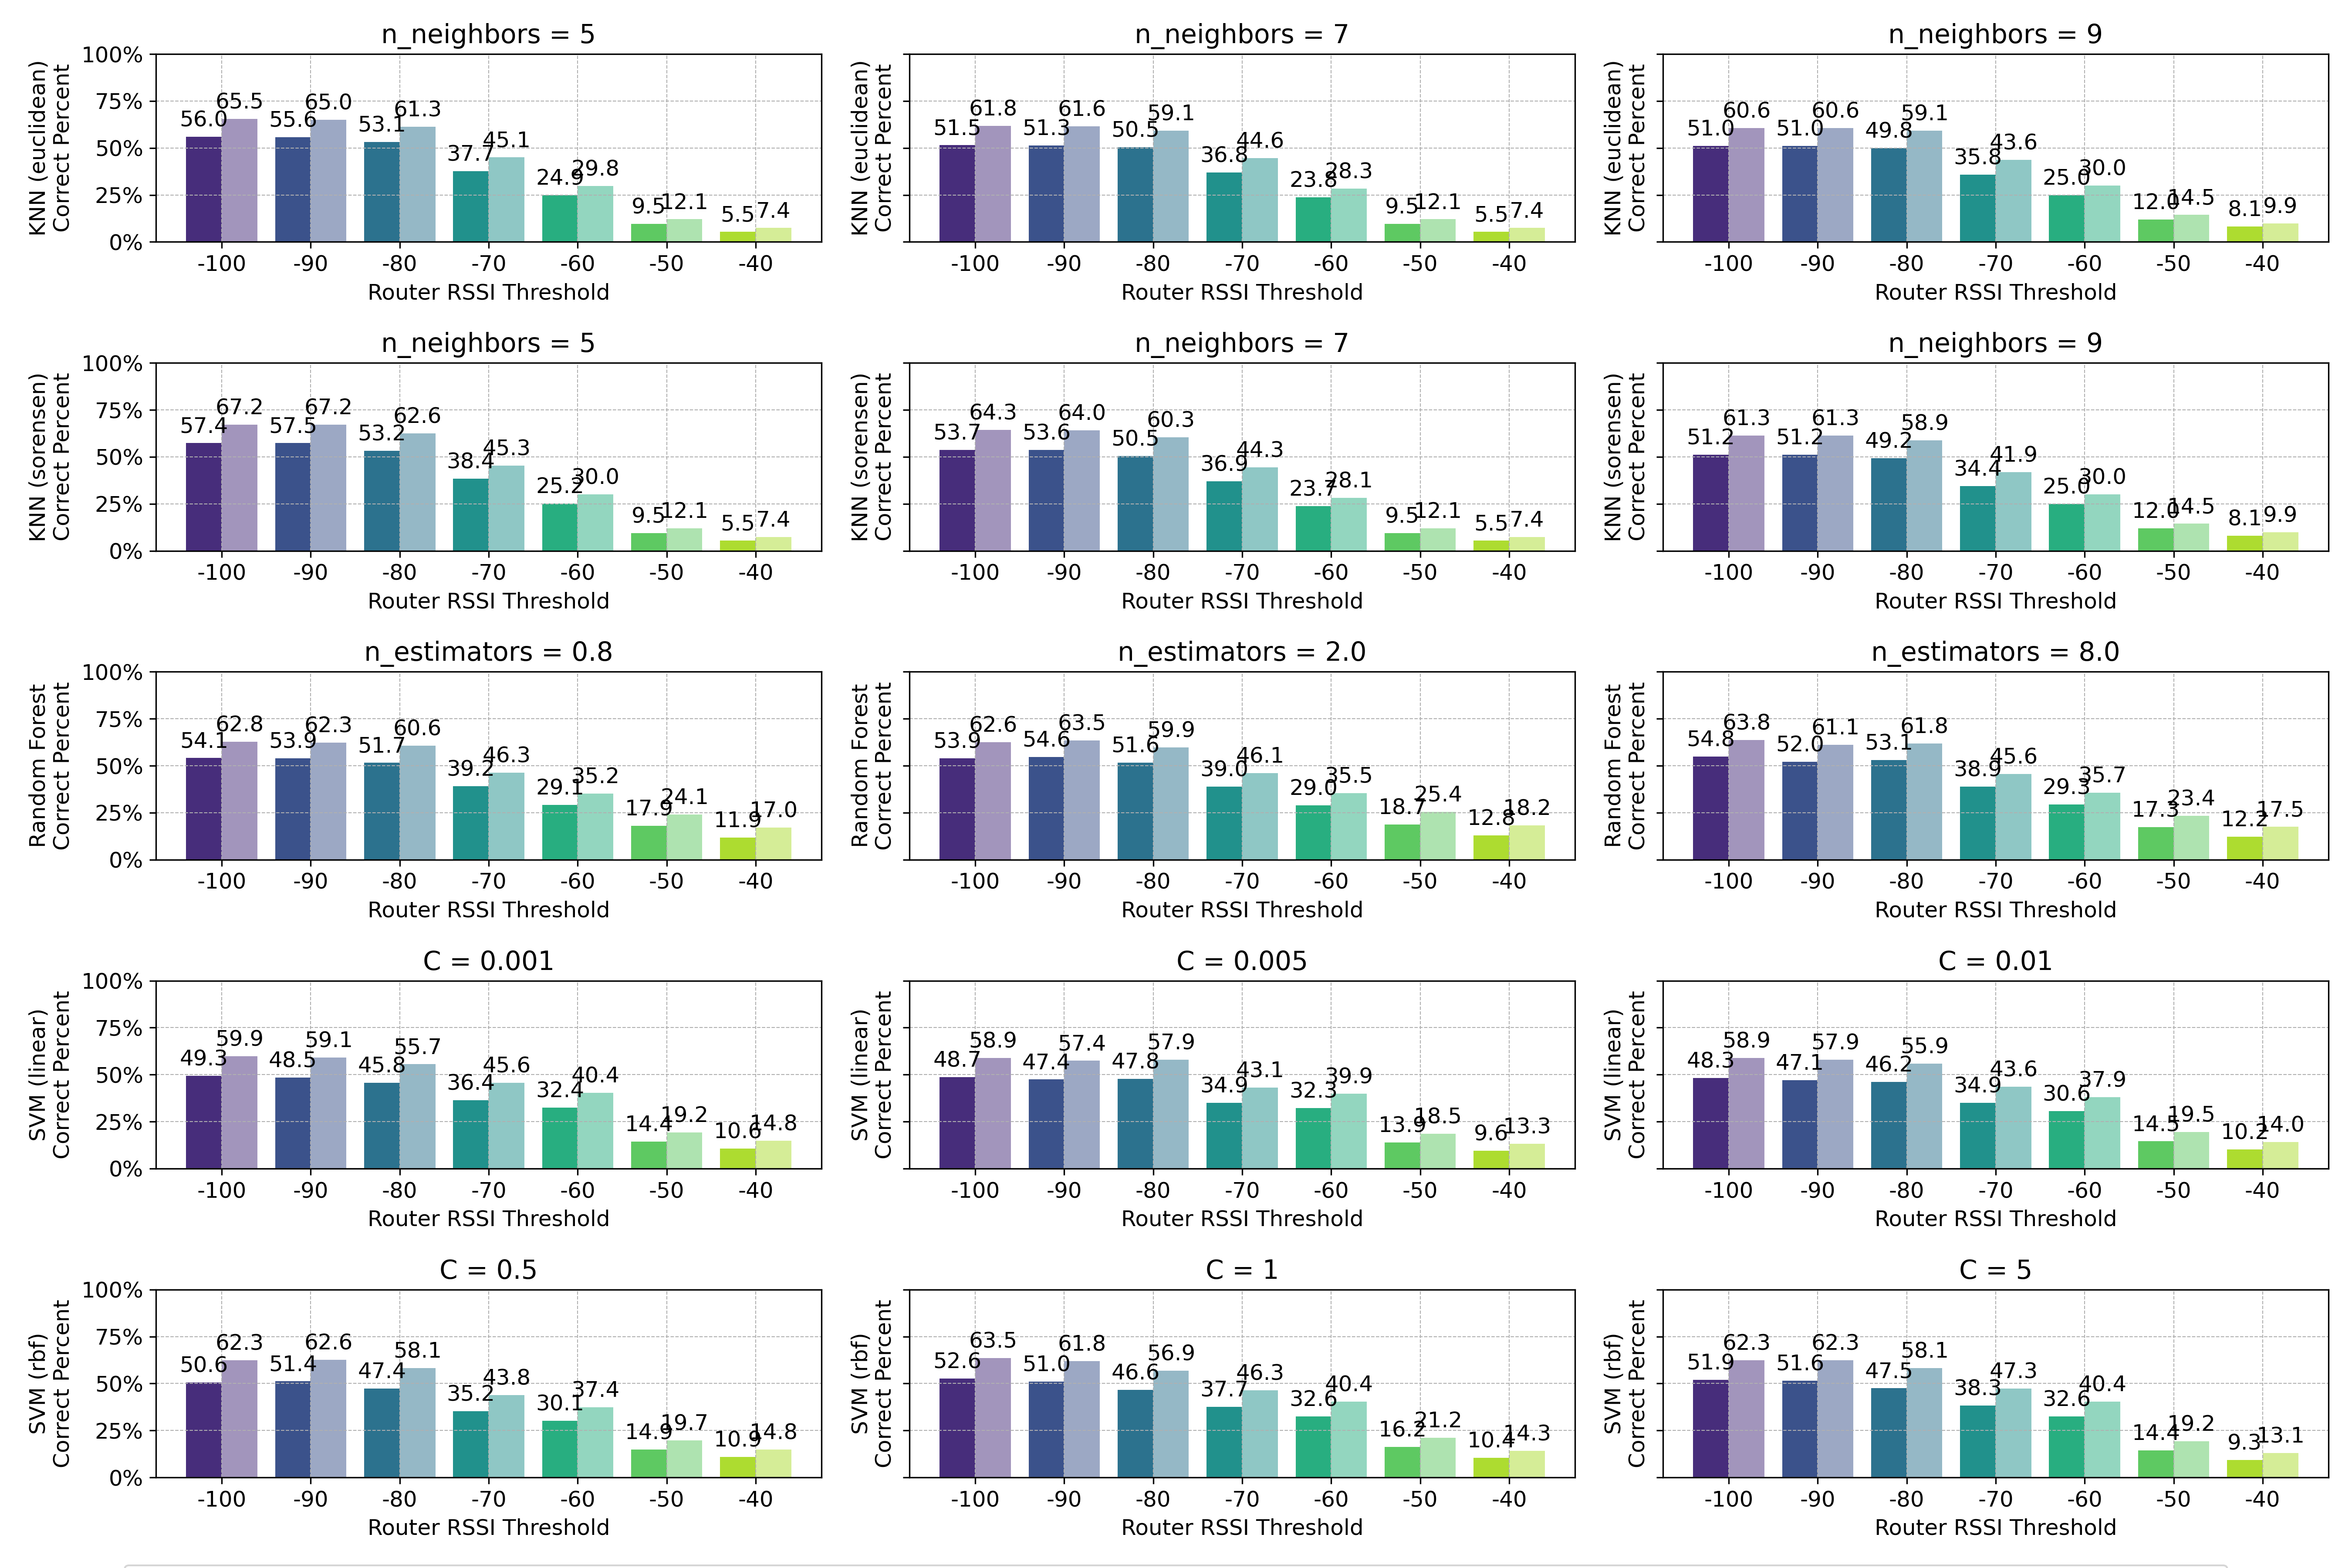
\includegraphics[width=0.8\textwidth]{images/09_router_rssi_threshold_03.png}
    \caption{Vergleich der durchschnittlichen Genauigkeit in Abhängigkeit des Schwellenwerts für die Mindestsignalstärke eines Routers}
    \label{fig:09_router_rssi_threshold_03}
\end{figure}

Wie in Abbildung \ref{fig:09_router_rssi_threshold_03} zu erkennen ist, führt die Ignorierung von Routern mit einem schwachen Signal zu keiner Verbesserung der Ergebnisse und die Genauigkeit der Vorhersagen nimmt in den meisten Fällen - abgesehen von ein paar Ausnahmen - linear ab. Bei den Ausnahmen (\gls{svm} mit RBF-Kernal und C = 0,5, Random Forest mit einer maximalen Anzahl von 2 Features und \gls{knn} mit der Sørensen-Distanz und k = 5) zeigt sich, dass die Genauigkeit bei einem Schwellenwert von -90 dBm leicht besser ist als die Genauigkeit bei einem Schwellenwert von -100 dBm. Insgesamt ist jedoch zu erkennen, dass die Ergebnisse bei einem Schwellenwert von -100 dBm am besten sind. Aus diesem Grund wird für die weiteren Untersuchungen ein Schwellenwert von -100 dBm verwendet.

\subsubsection{Skalierung von RSSI-Werten}

Im fünften Schritt der Datenaufbereitung wird untersucht, ob die Skalierung der RSSI-Werte die Genauigkeit der Modelle verbessern kann. Die Idee hinter der Werteskalierung stammt aus dem Paper \textit{Comprehensive analysis of distance and similarity measures for Wi-Fi fingerprinting indoor positioning systems} und basiert auf der Erkenntnis, dass die RSSI-Werte nicht linear verteilt sind (siehe Kapitel \ref{pfadverlustmodell}). Dafür werden wie in dem Paper beschrieben drei verschiedene Skalierungsmethoden implementiert und mit den bisher nicht skalierten Werten verglichen.\myfootcite{TorresSospedra2015WiFi}{S. 9269}

Die drei Skalierungsmethoden sind:

\begin{enumerate}
    \item \textbf{Lineare Normalisierung}
    \item \textbf{Exponentielle Skalierung}
    \item \textbf{Potenzierte Skalierung}
\end{enumerate}

% \subsubsection{Formeln}

% % Quelle XX: Comprehensive analysis of distance and similarity measures for Wi-Fi fingerprinting indoor positioning systems

% Die Idee hinter der Werteskalierung stammt aus der Quelle XX und basiert auf der Erkenntnis, dass die RSSI-Werte nicht linear verteilt sind. Durch eine geeignete Skalierung kann der Zusammenhang zwischen Entfernung und RSSI-Wert besser abgebildet werden. In der vorliegenden Arbeit wurden drei Skalierungsmethoden aus der Quelle XX implementiert und verglichen.

Grundlage jeder Skalierung ist die positive Darstellung der Werte. Hierfür wird jeder Wert in den Trainings- und Testdaten mit dem niedrigsten gemessenen RSSI-Wert minus 1 dBm (\(\text{min}\)) subtrahiert:

\begin{equation}
    \text{Positiv}_i(x) = \text{RSS}_i - (\text{min})
    \label{eq:positive_values_representation}
\end{equation}

Durch diese Skalierung werden alle RSSI-Werte positiv dargestellt und der niedrigste Wert ist 1 dBm.

\textbf{Lineare Normalisierung:}

Die linear normalisierten Werte werden berechnet mit:

\begin{equation}
    \text{Normiert}_i(x) = \frac{\text{Positiv}_i(x)}{-\text{min}}
    \label{eq:linear_normalized_values}
\end{equation}

und befeinden nach der Skalierung in dem Wertebereich [0, 1].

\textbf{Exponentielle Skalierung:}

Die exponentiell skalierten Werte werden berechnet mit:

\begin{equation}
    \text{Exponential}_i(x) = \frac{\exp\left(\frac{\text{Positiv}_i(x)}{\alpha}\right)}{\exp\left(\frac{-\text{min}}{\alpha}\right)}
    \label{eq:exponential_representation}
\end{equation}

und \(\alpha = 24\).

Die Auswahl dieses Wertes für den Parameter \(\alpha\) basiert auf den Ergebnissen aus dem Paper {Comprehensive analysis of distance and similarity measures for Wi-Fi fingerprinting indoor positioning systems}.\myfootcite{TorresSospedra2015WiFi}{S. 9269}

\textbf{Potenzierte Skalierung:}

Die potenzierten Werte werden unter Verwendung von \(\beta = e\) und der Formel:

\begin{equation}
    \text{Potenziert}_i(x) = \left(\frac{\text{Positiv}_i(x)}{-\text{min}}\right)^{\beta}
    \label{eq:powered_representation}
\end{equation}

berechnet. Diese Auswahl basiert ebenfalls auf den Ergebnissen aus dem Paper \textit{Comprehensive analysis of distance and similarity measures for Wi-Fi fingerprinting indoor positioning systems}.\myfootcite{TorresSospedra2015WiFi}{S. 9269}

In Abbildung \ref{fig:value_scaling_strategies_ignore_10} sind die verschiedenen Skalierungsmethoden dargestellt. Für diese exemplarische Darstellung wurden RSSI-Werte zwischen -100 dBm und -1 dBm in einem Interval von 1 dBm betrachtet.

\begin{figure}[H]
    \centering
    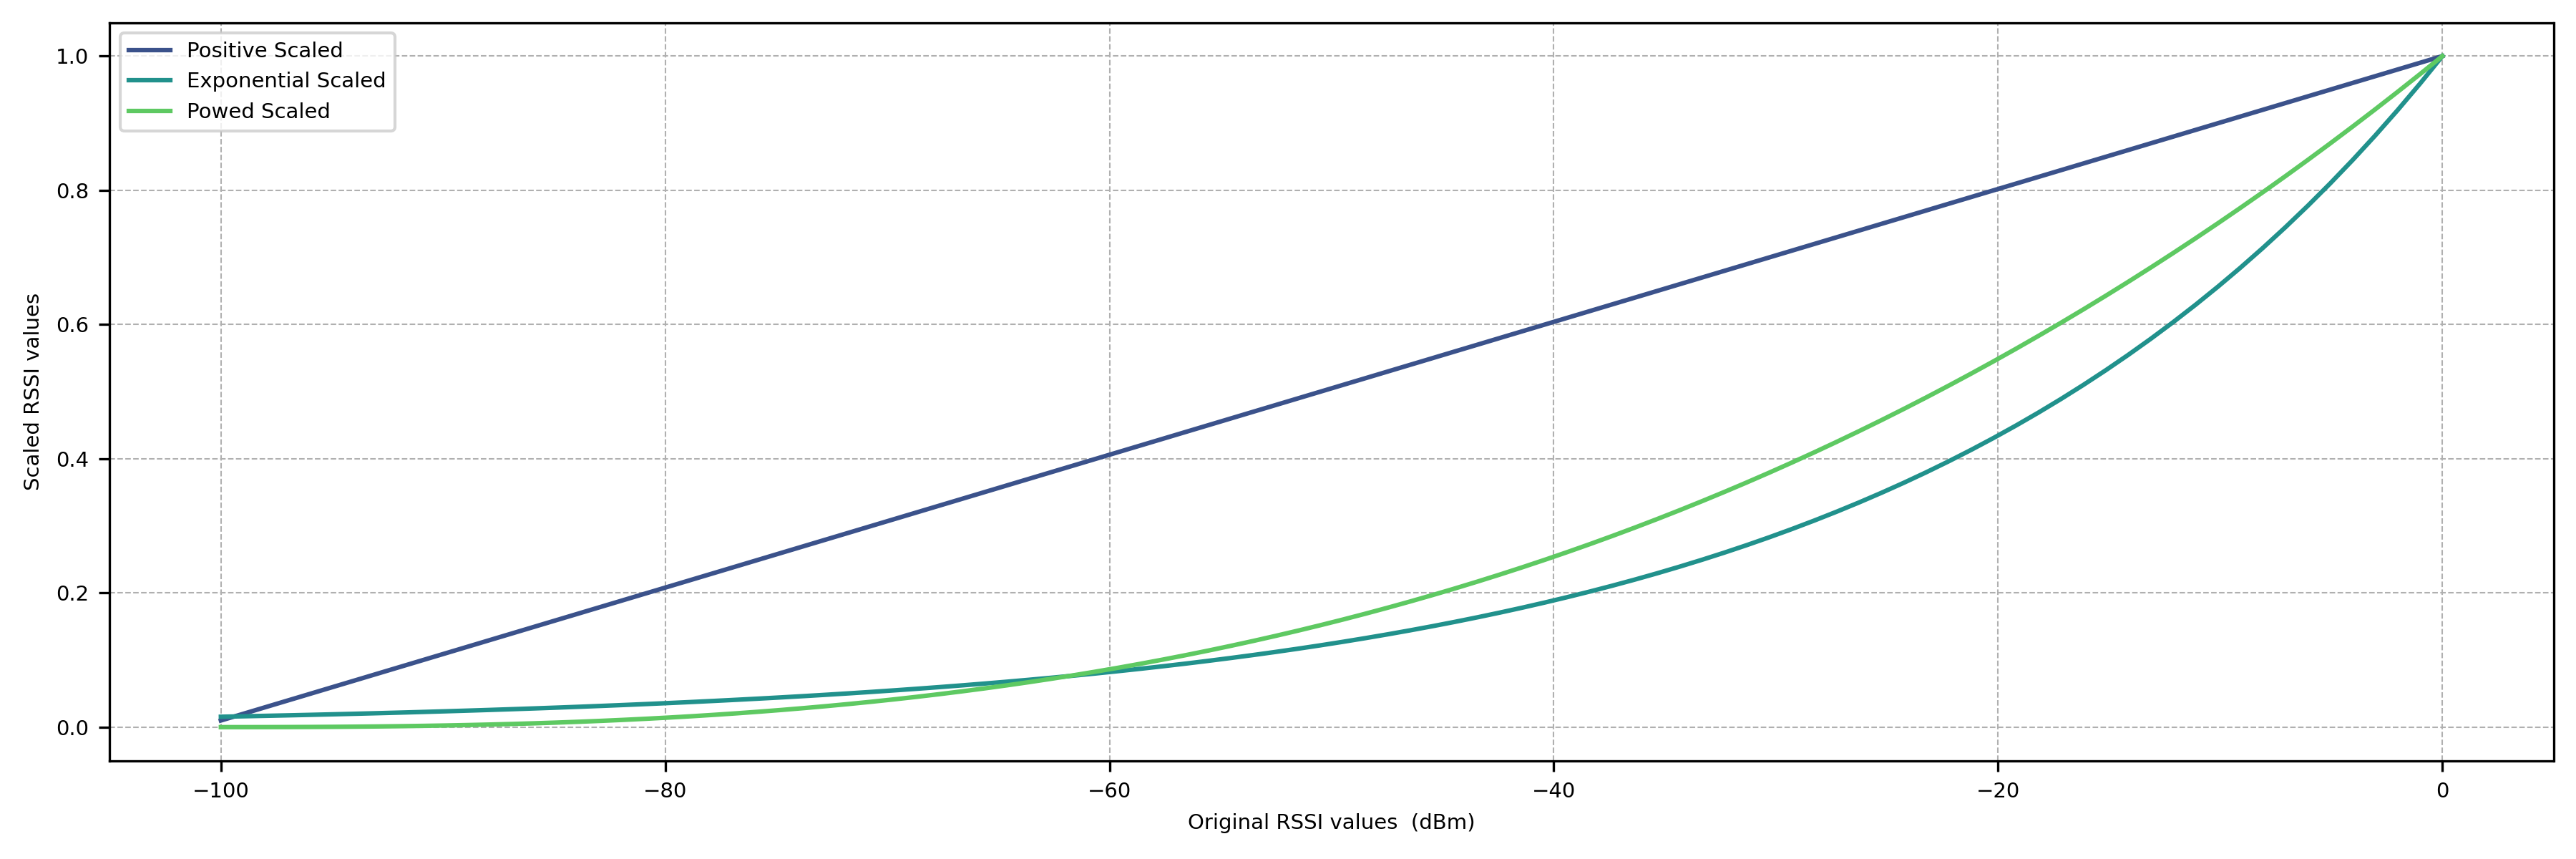
\includegraphics[width=0.8\textwidth]{images/plot_scaling_strategies.png}
    \caption{Darstellung der verschiedenen Skalierungsmethoden}
    \label{fig:value_scaling_strategies_ignore_10}
\end{figure}

Da in dem \gls{knn}-Modell die Distanzen zur Bestimmung der Räume auf den RSSI-Werten basieren und die Skalierung dieser Werte den Wertebereich beeinflusst hat, wird zunächst überprüft, ob die gewählte Gewichtung (\texttt{weights = distance}) weiterhin optimal ist. Dazu wurde der \gls{knn}-Algorithmus mit beiden Gewichtungsfunktionen und beiden Distanzmetriken jeweils mit linearer Normalisierung, exponentieller Skalierung, potenzierter Skalierung und den unskalierten Werten verglichen.

\begin{figure}[H]
    \centering
    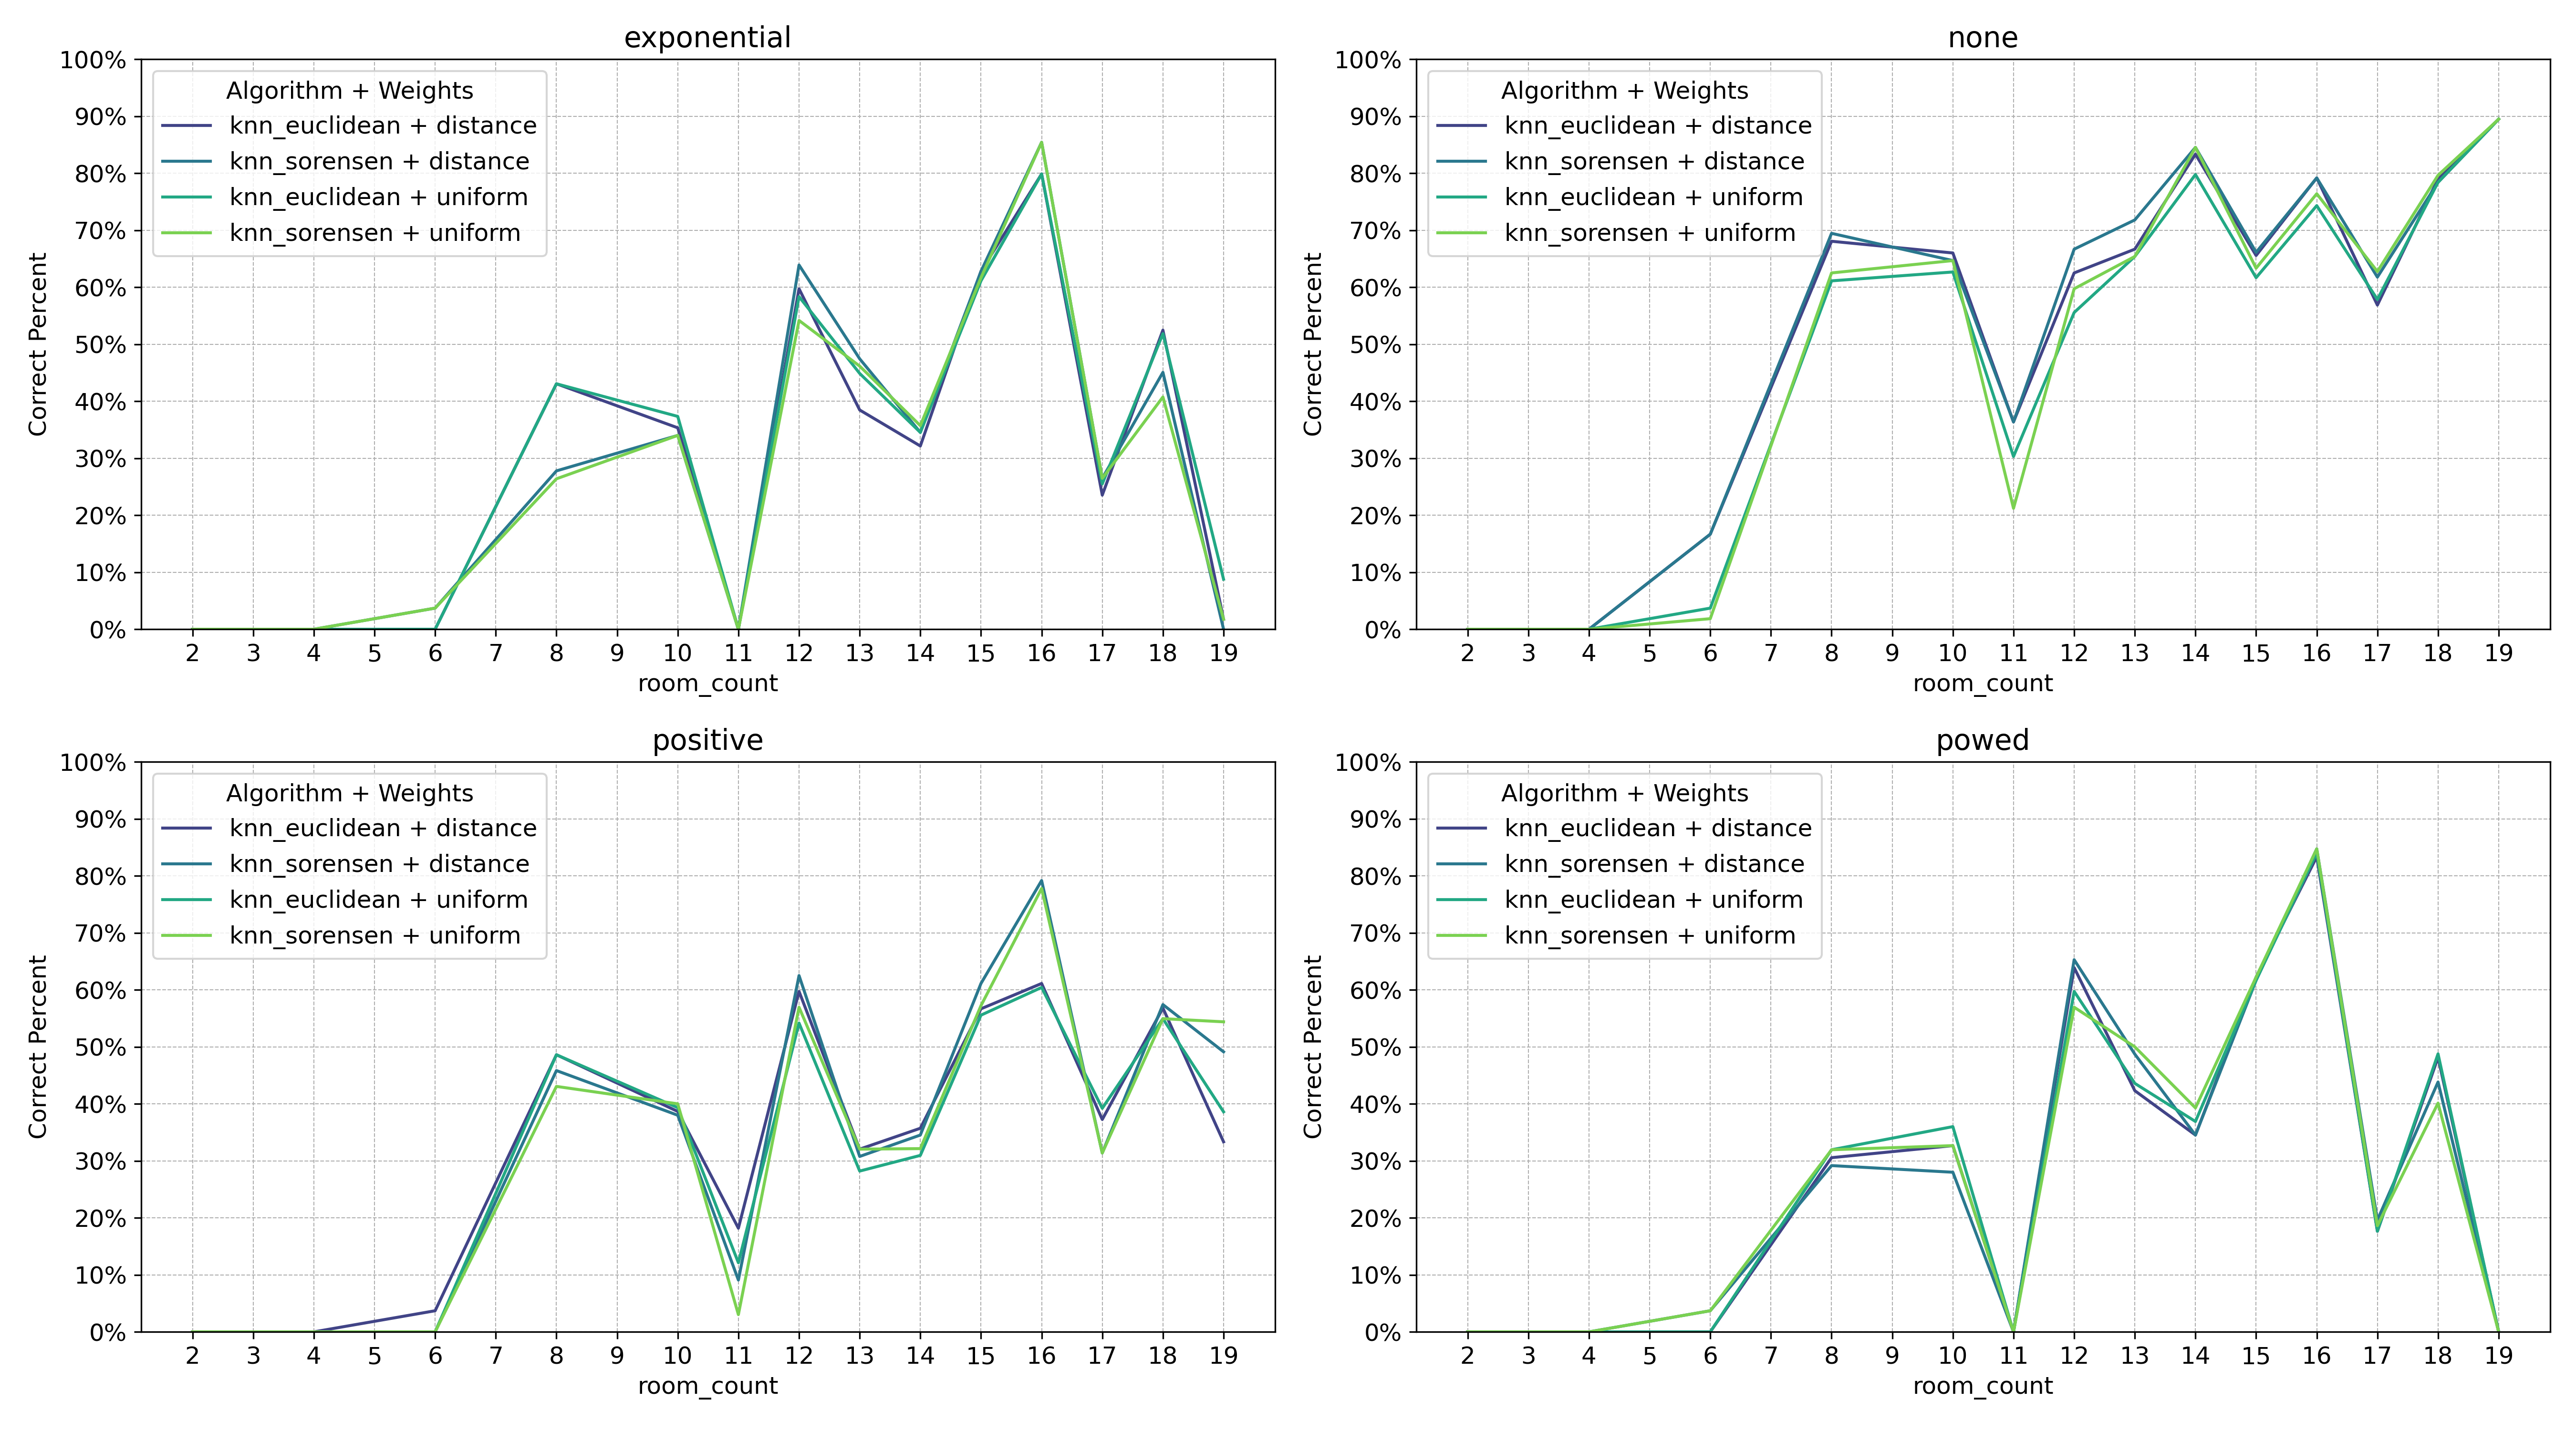
\includegraphics[width=0.8\textwidth]{images/10_knn_weights_value_scaling_strategy_03.png}
    \caption{Vergleich des \gls{knn}-Algorithmus mit den verschiedenen Skalierungsmethoden und beiden Gewichtungsfunktionen}
    \label{fig:10_knn_weights_value_scaling_strategy_03}
\end{figure}

Wie in Abbildung \ref{fig:10_knn_weights_value_scaling_strategy_03} zu erkennen ist, zeigen die Ergebnisse unabhängig von der gewählten Distanzmetrik und der Gewichtungsfunktion einen ähnlichen Verlauf innerhalb jeder Skalierungsstrategie. Auffällig ist jedoch, dass bei der exponentiellen und der potenzierten Skalierung die Genauigkeit in Räumen mit mehr als 16 Messungen deutlich abnimmt, wobei der Rückgang bei der potenzierten Skalierung weniger stark ausgeprägt ist. Zudem gibt es leichte Unterschiede zwischen den Distanzmetriken: Bei der exponentiellen Skalierung schneidet die Sørensen-Distanz in Räumen mit 8 Messungen schlechter ab und bei der positiven Skalierung in Räumen mit 16 Messungen, jeweils im Vergleich zur euklidischen Distanz.

\begin{figure}[H]
    \centering
    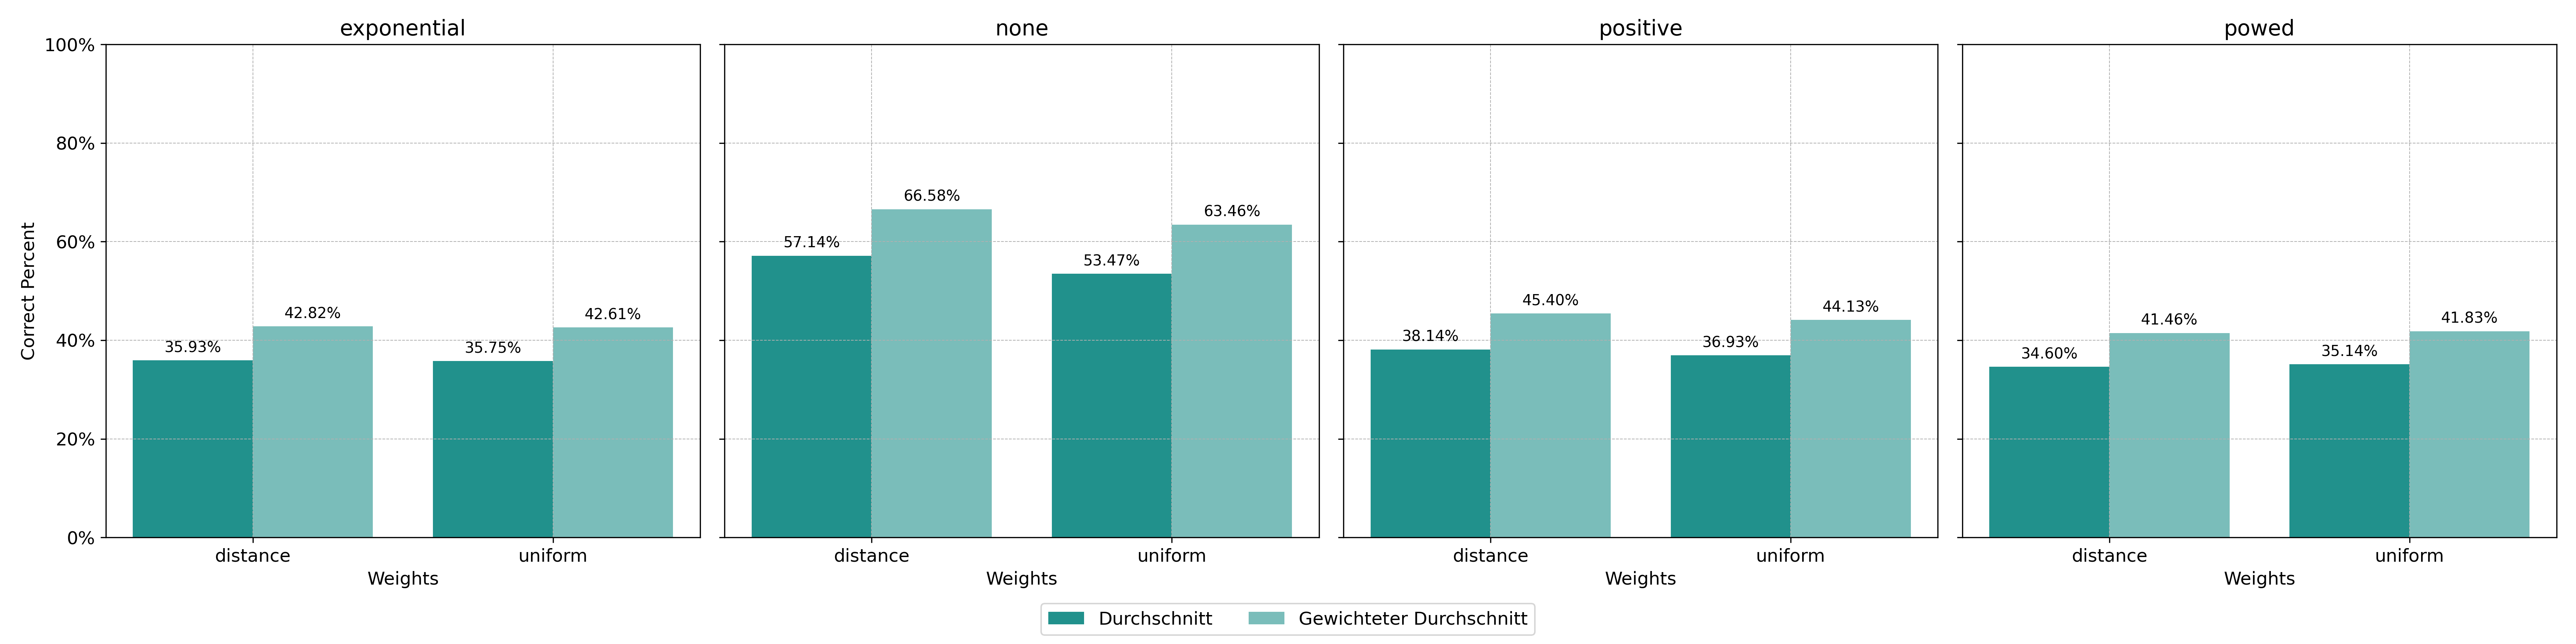
\includegraphics[width=0.8\textwidth]{images/10_knn_weights_value_scaling_strategy_02.png}
    \caption{Vergleich der durchschnittlichen Genauigkeit des \gls{knn}-Algorithmus in Bezug auf die verschiedenen Skalierungsmethoden und beide Gewichtungsfunktionen}
    \label{fig:10_knn_weights_value_scaling_strategy_02}
\end{figure}

Wenn man sich die durschnittliche Genauigkeit der beiden Distanzmetriken in Abhängigkeit der Skalierungsstrategie ansieht, zeigt sich in Abbildung \ref{fig:10_knn_weights_value_scaling_strategy_02}, dass abgesehen von der potenzierten Skalierung in jedem Fall die gewichtete Distanzfunktion (\texttt{weights = distance}) besser abschneidet und dass die besten Ergebnisse mit den unskalierten Werten erzielt werden konnten. Aus diesem Grund wird für die weiteren Untersuchungen weiterhin gewichtete Distanzfunktion verwendet.

% In Abbildung \ref{fig:7_value_scaling_strategy_02} folgendes zu erkennen:

% \begin{itemize}
%     \item In den meisten fällen sehr ähnlicher Verlauf --> Es gibt Unterschiede bei den Skalierungsmethoden, aber bei den Skalierungsmethoden sind die Ergebnisse bei euclidean/sorensen und distance/uniform sehr ähnlich
%     \item Bei exponential: distance ist besser als uniform bei wenigen Messungen pro Raum
%     \item Bei none: distanz ist etwas besser als uniform bei wenigeren Messungen. Abstand nimmt aber ab mit der Anzahl an Messungen
%     \item Bei exponential, powed (und auch leicht bei positive): Nimmt die Genauigkeit mit zunehmender Anzahl an Messungen wieder ab. Bisher hatten die Räume mit den meisten Messungen immer die größten Genauigkeiten. In diesem Fall haben die Räume mit 16 Messungen die höchste Genauigkeit und danach nimmt es wieder ab. Bei exponential und powed ist die Genauzigkeit bei n = 19 sogar wieder bei fast allen Kombinationen aus distance und weights bei 0\%!
% \end{itemize}

Bei der Untersuchung der weiteren Modelle (siehe Abbildungen \ref{fig:7_value_scaling_strategy_02} und \ref{fig:7_value_scaling_strategy_03}) zeigt sich, dass die nicht skalierten Werte in den meisten Fällen bessere Ergebnisse liefern als die skalierten. Es ist auch ersichtlich, dass bei den skalierten Werten die Genauigkeit zwar zunächst mit zunehmender Anzahl an Messungen pro Raum ansteigt, aber ab einem bestimmten Punkt (ungefähr bei 16 Messungen pro Raum) wieder deutlich abnimmt. Aufgrund dieser Beobachtungen wird in den weiteren Untersuchungen auf die Skalierung der RSSI-Werte verzichtet.

\begin{figure}[H]
    \centering
    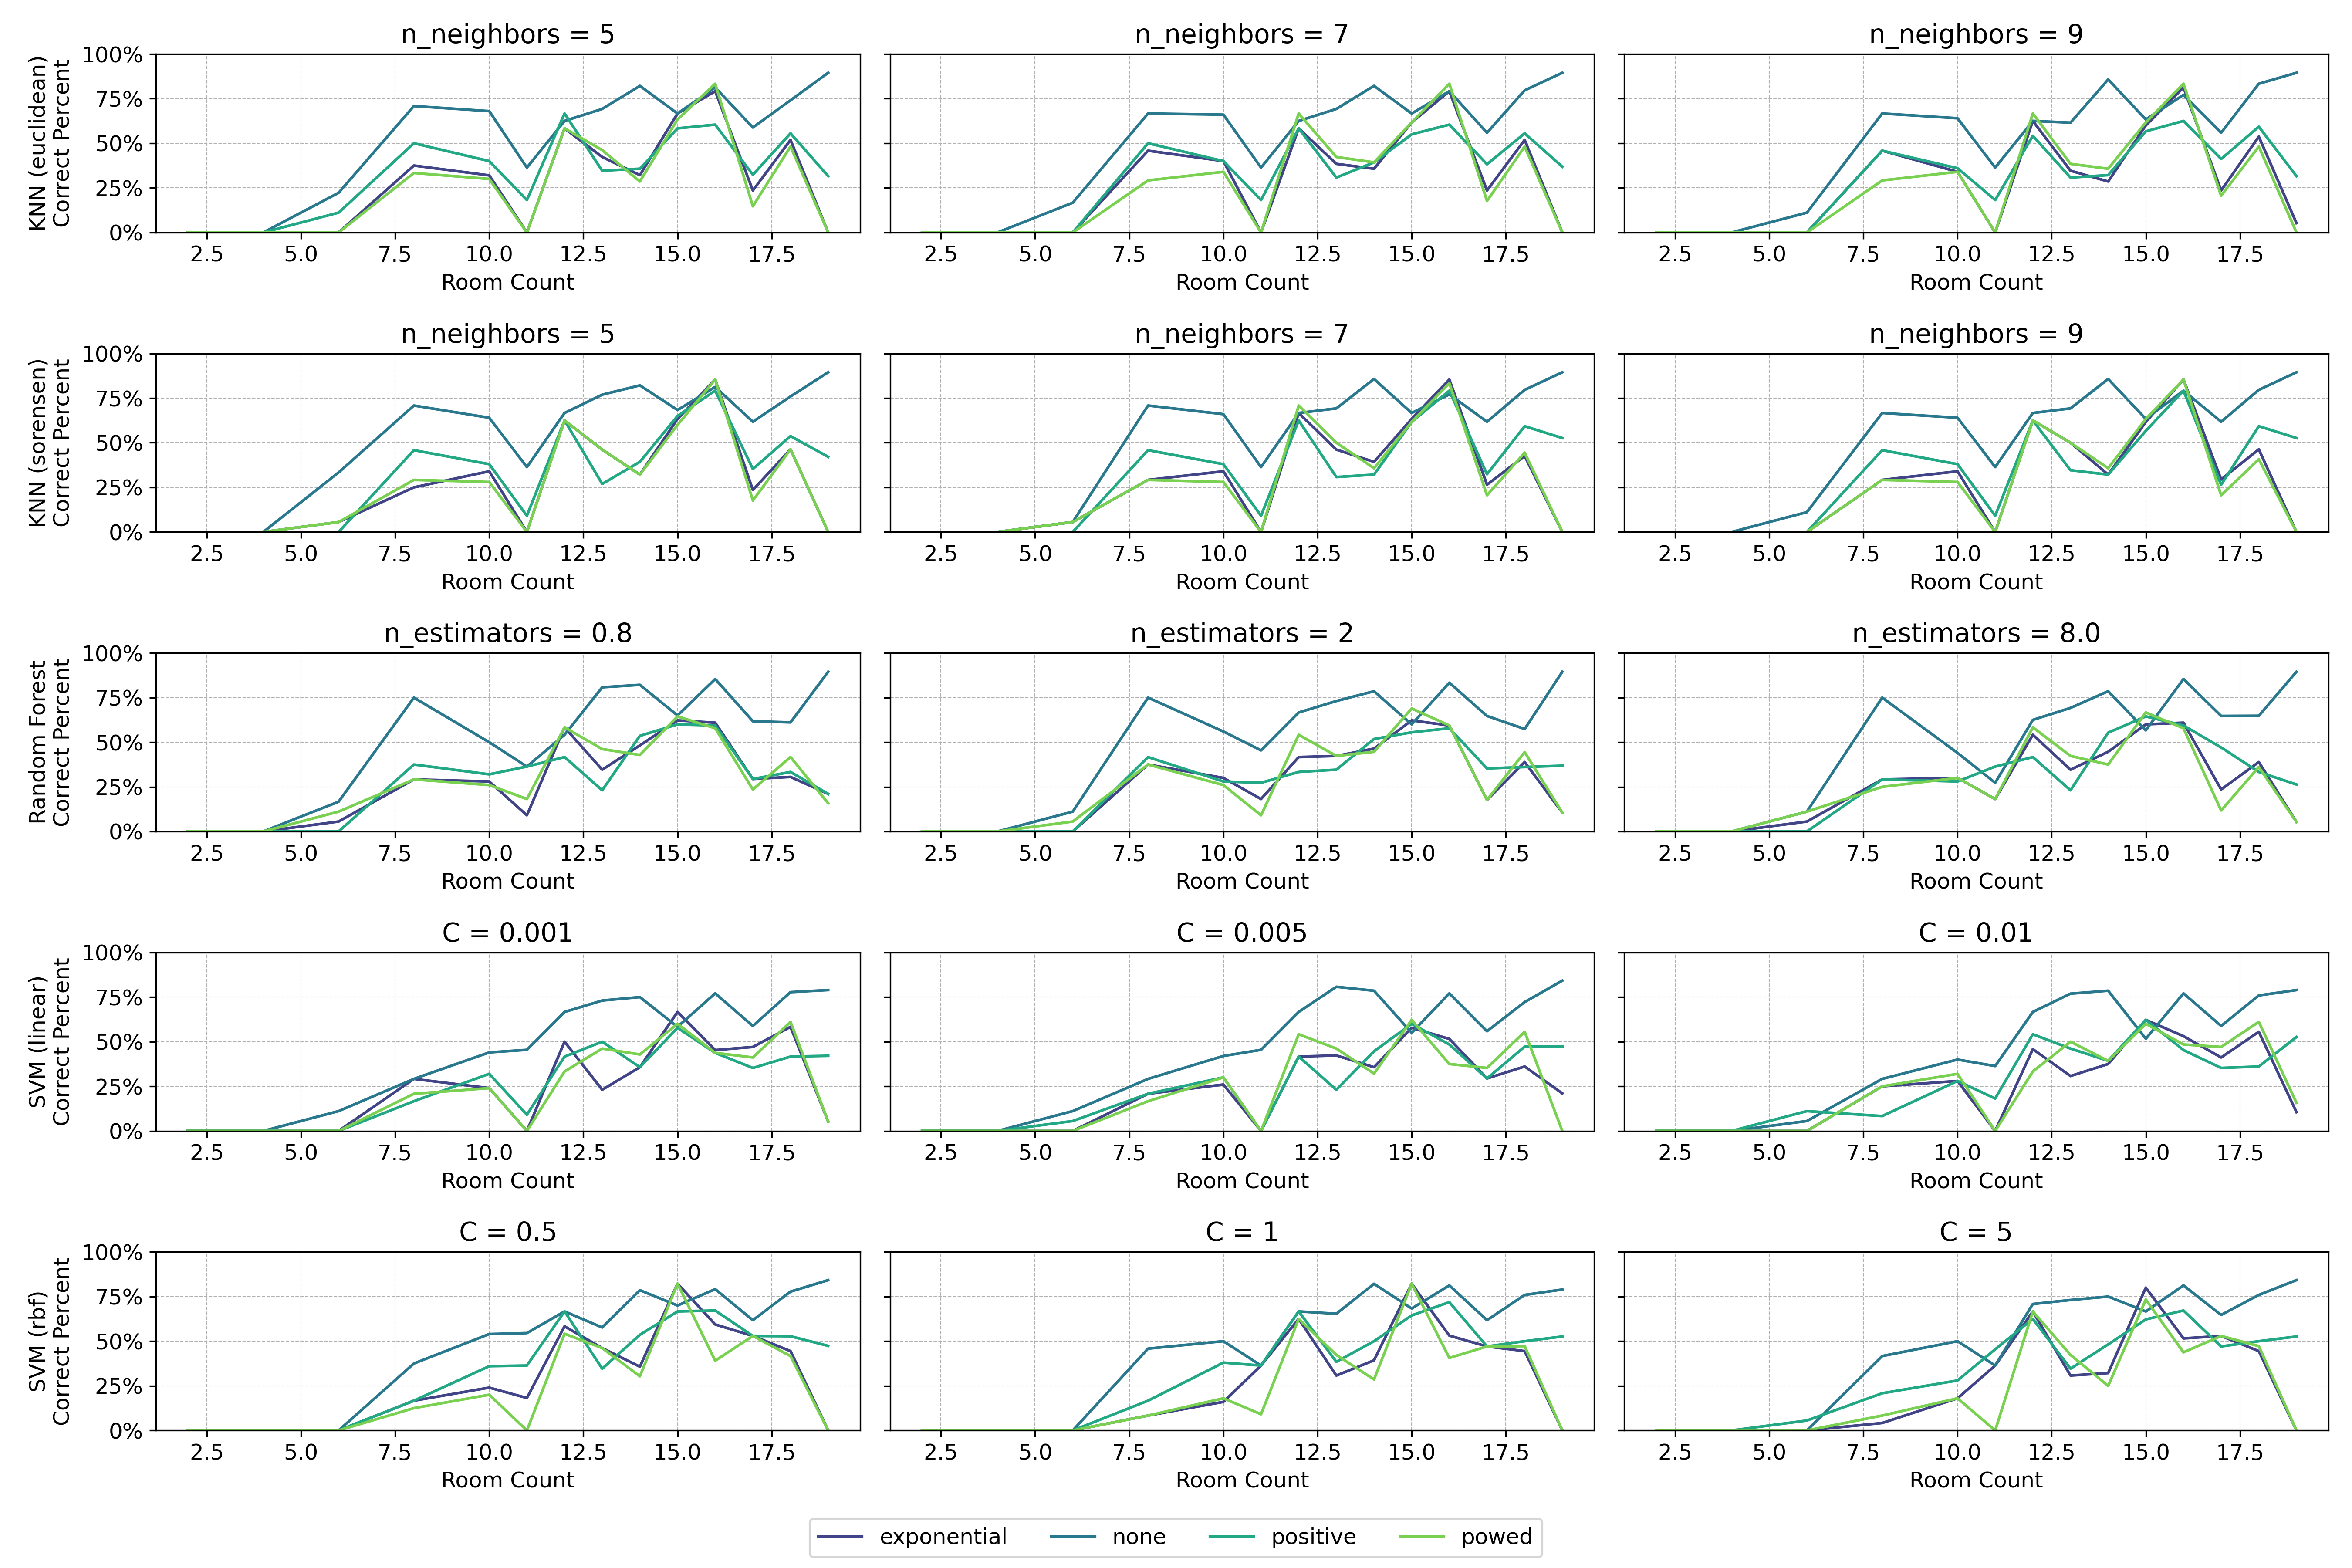
\includegraphics[width=0.8\textwidth]{images/11_value_scaling_strategy_02.png}
    \caption{Vergleich der Genauigkeit in Abhängigkeit der Skalierungsstrategeien}
    \label{fig:7_value_scaling_strategy_02}
\end{figure}

\begin{figure}[H]
    \centering
    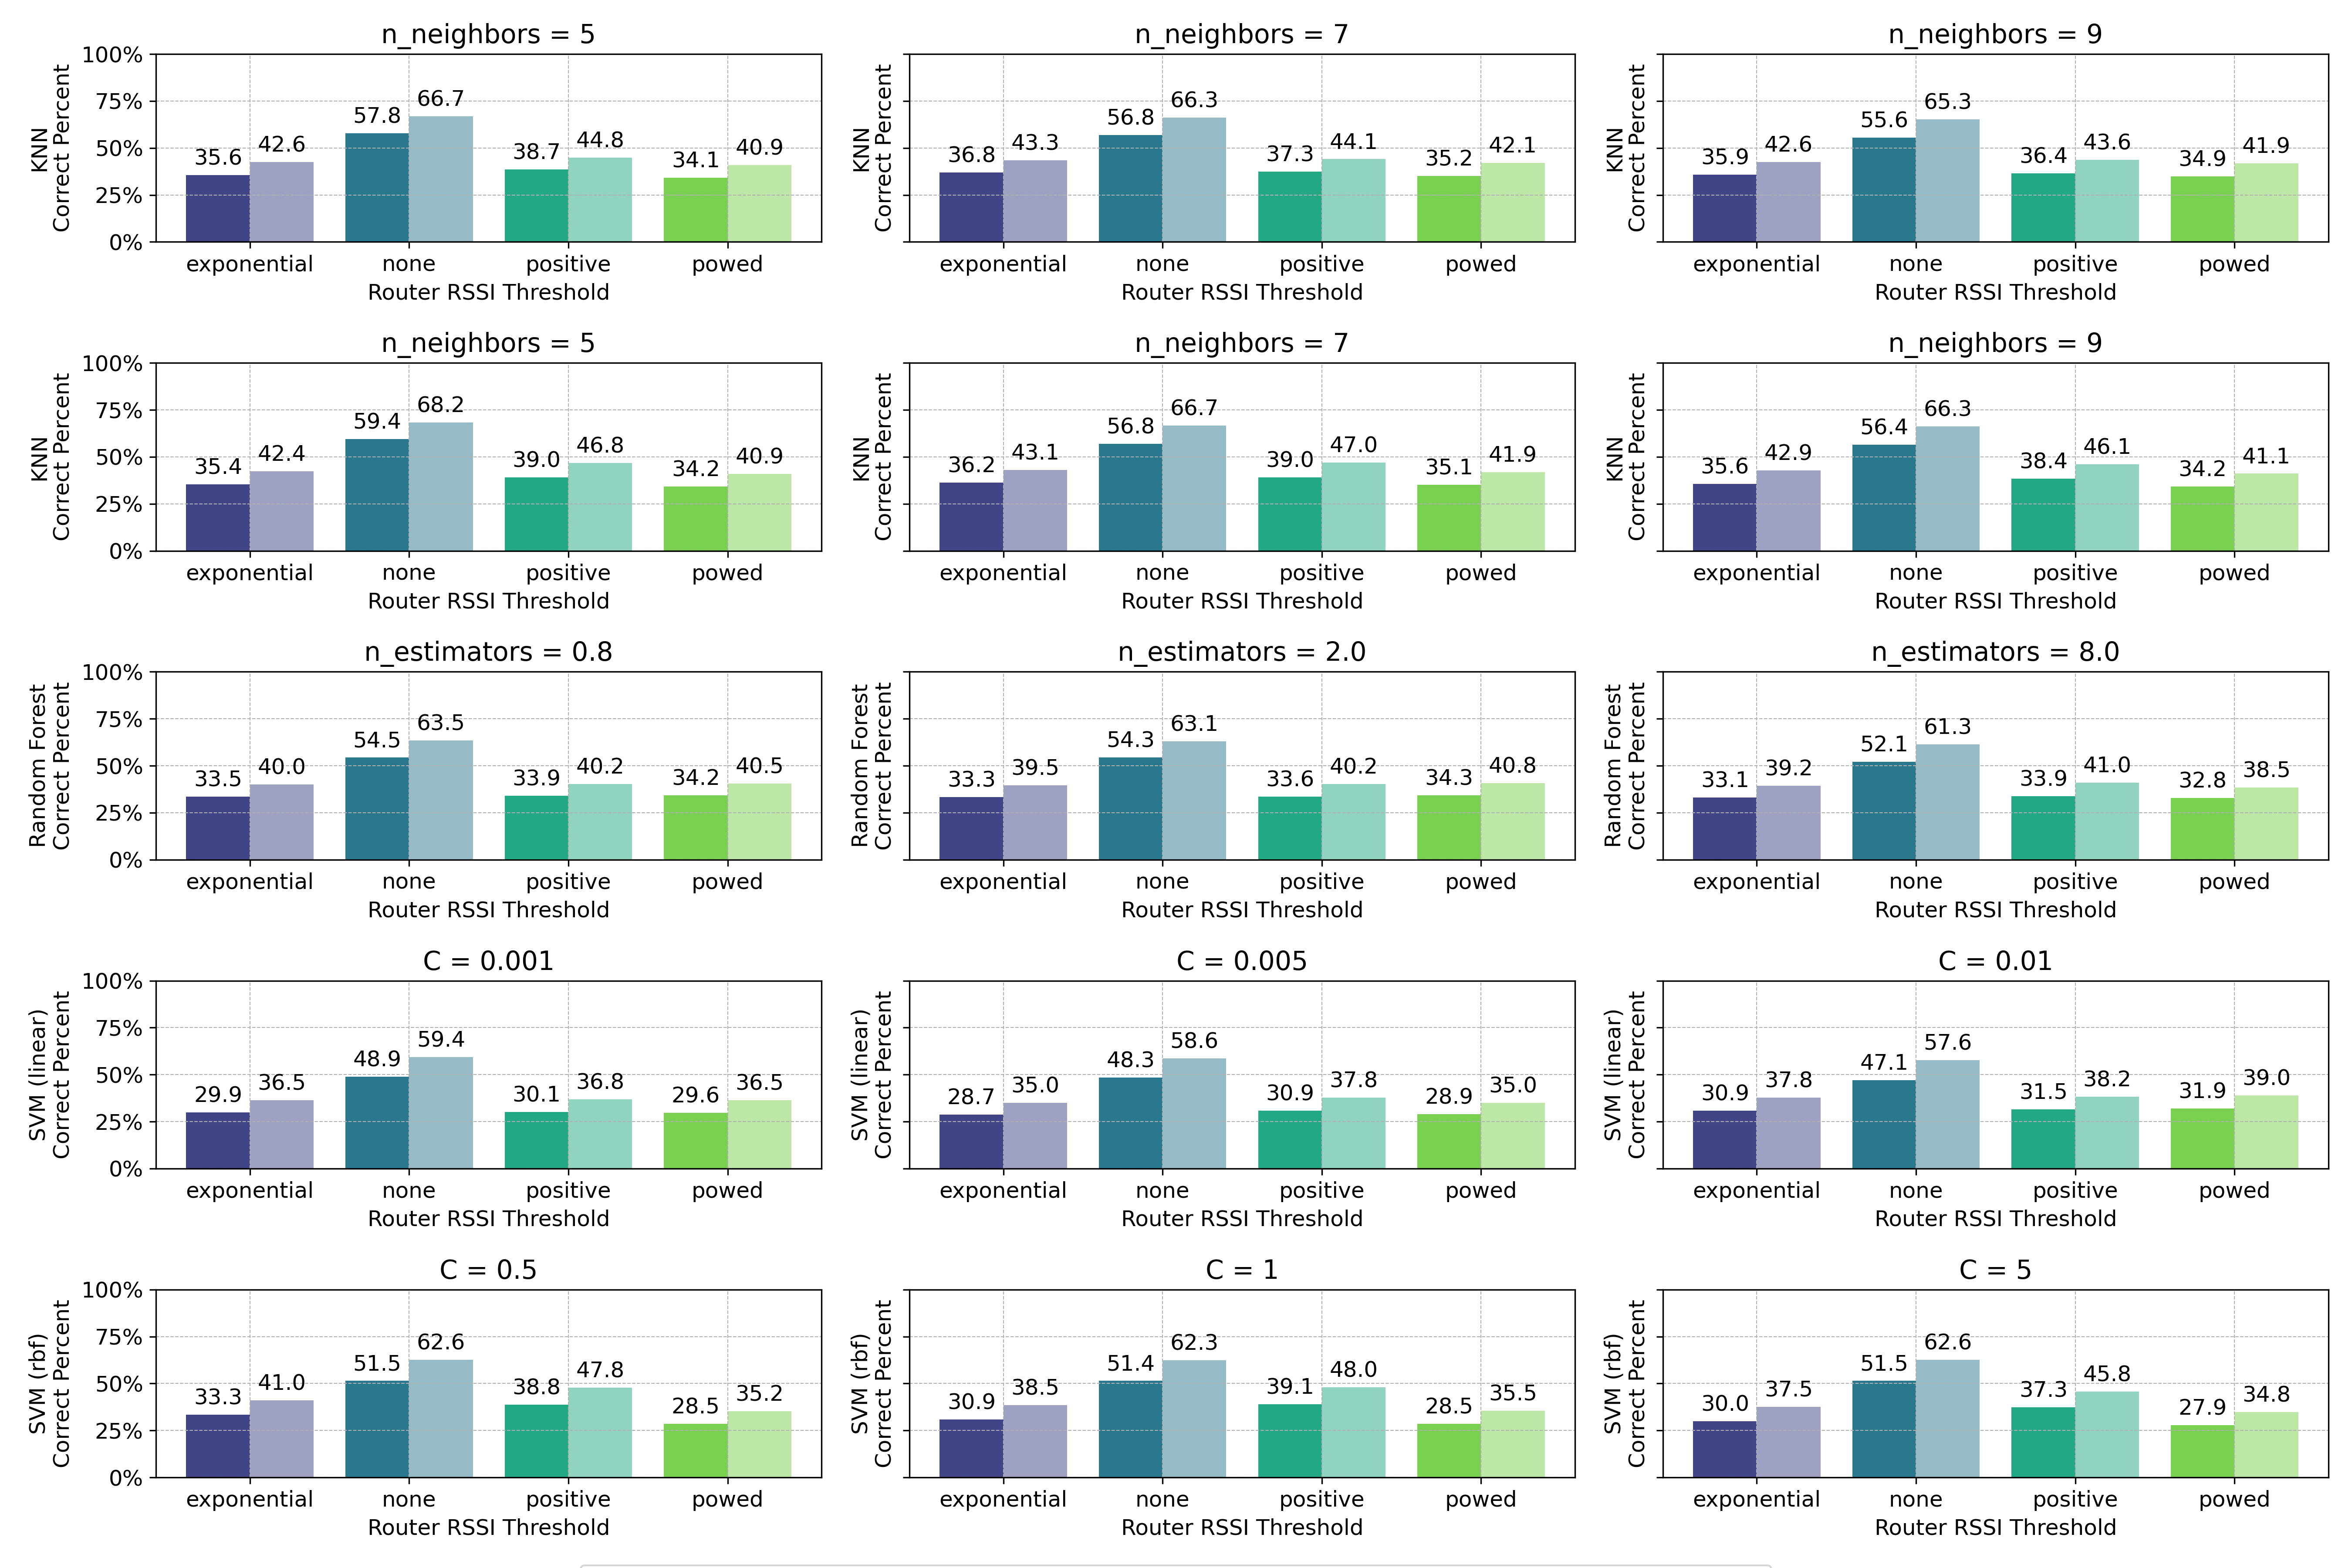
\includegraphics[width=0.8\textwidth]{images/11_value_scaling_strategy_03.png}
    \caption{Vergleich der durchschnittlichenGenauigkeit in Abhängigkeit der Skalierungsstrategeien}
    \label{fig:7_value_scaling_strategy_03}
\end{figure}

Insgesamt konnten die besten Ergebnisse mit dem \gls{knn}-Modell unter Verwendung der Sørensen-Distanzmetrik, der gewichteten Distanzfunktion und \( k  = 5 \) erzielt werden.

\section{Erweiterte Untersuchungen} \label{erweiterte_untersuchungen}

In den Kapiteln \ref{untersuchungen} und \ref{datenaufbereitung} konnte ermittelt werden, dass bei den Testdaten der \gls{knn}-Algorithmus mit der Sørensen Distanzmetrik und einem Wert von \( k  = 5 \) die besten Ergebnisse erzielen konnte. In dem folgenden Kapitel wird nun konkreter untersucht, wie sich die Anzahl der Messungen auf die Genauigkeit auswirkt und ob eine Verbesserung der Vorhersagegenauigkeit erzielt werden kann, wenn zusätzliche Messungen an Orten durchgeführt werden, die nicht zu den Räumen gehören. Die Idee dabei ist, dass durch Messungen an Orten, die nicht zu den Räumen gehören, die Unterscheidung zwischen den Räumen verbessert werden kann und falsche Vorhersagen reduziert werden können. Für die Orte außerhalb der Räume wurde der Flur zwischen den Räumen ausgewählt. Sollte bei der Raumbestimmung ein Flur vorhergesagt werden, so wird die Vorhersage als nicht falsch gewertet.

Um diese Hypothese zu überprüfen, wurden in vier nebeneinander liegenden Räumen (WH C 335, WH C 351, WH C 352 und WH C 353) sowie in dem Flur zwischen diesen Räumen, weitere Messungen in dem Zeitraum vom 7. Juli 2024 bis zum 19. Juli 2024 durchgeführt, sodass für jeden dieser Räume und den Flurbereich 20 Fingerprints vorhanden sind. Um den Einfluss der Anzahl der Messungen auf die Genauigkeit der Vorhersagen zu untersuchen, wurde für jeden der vier Räume eine Raumvorhersage erstellt. Dabei wurden für jede Messung eine Vorhersage getroffen und alle möglichen Kombinationen aus der Anzahl der Fingerprints pro Raum \((1, 3, 5, \ldots, 19)\) und der Anzahl der Messungen im Flur \((0, 1, 3, 5, \ldots, 19)\) berücksichtigt.

In der Abbildung \ref{fig:12_corridor_01} ist dargestellt in wie vielen Fällen und unter welcher Anzahl der Messungen pro Raum und auf dem Flur die Raumvorhersage korrekt war (linke Heatmap), in wie vielen Fällen Vorhersage korrekt oder nicht falsch war (mittlere Heatmap) und in wie vielen Fällen der Flur vorhergesagt wurde (rechte Heatmap).

\begin{figure}[H]
    \centering
    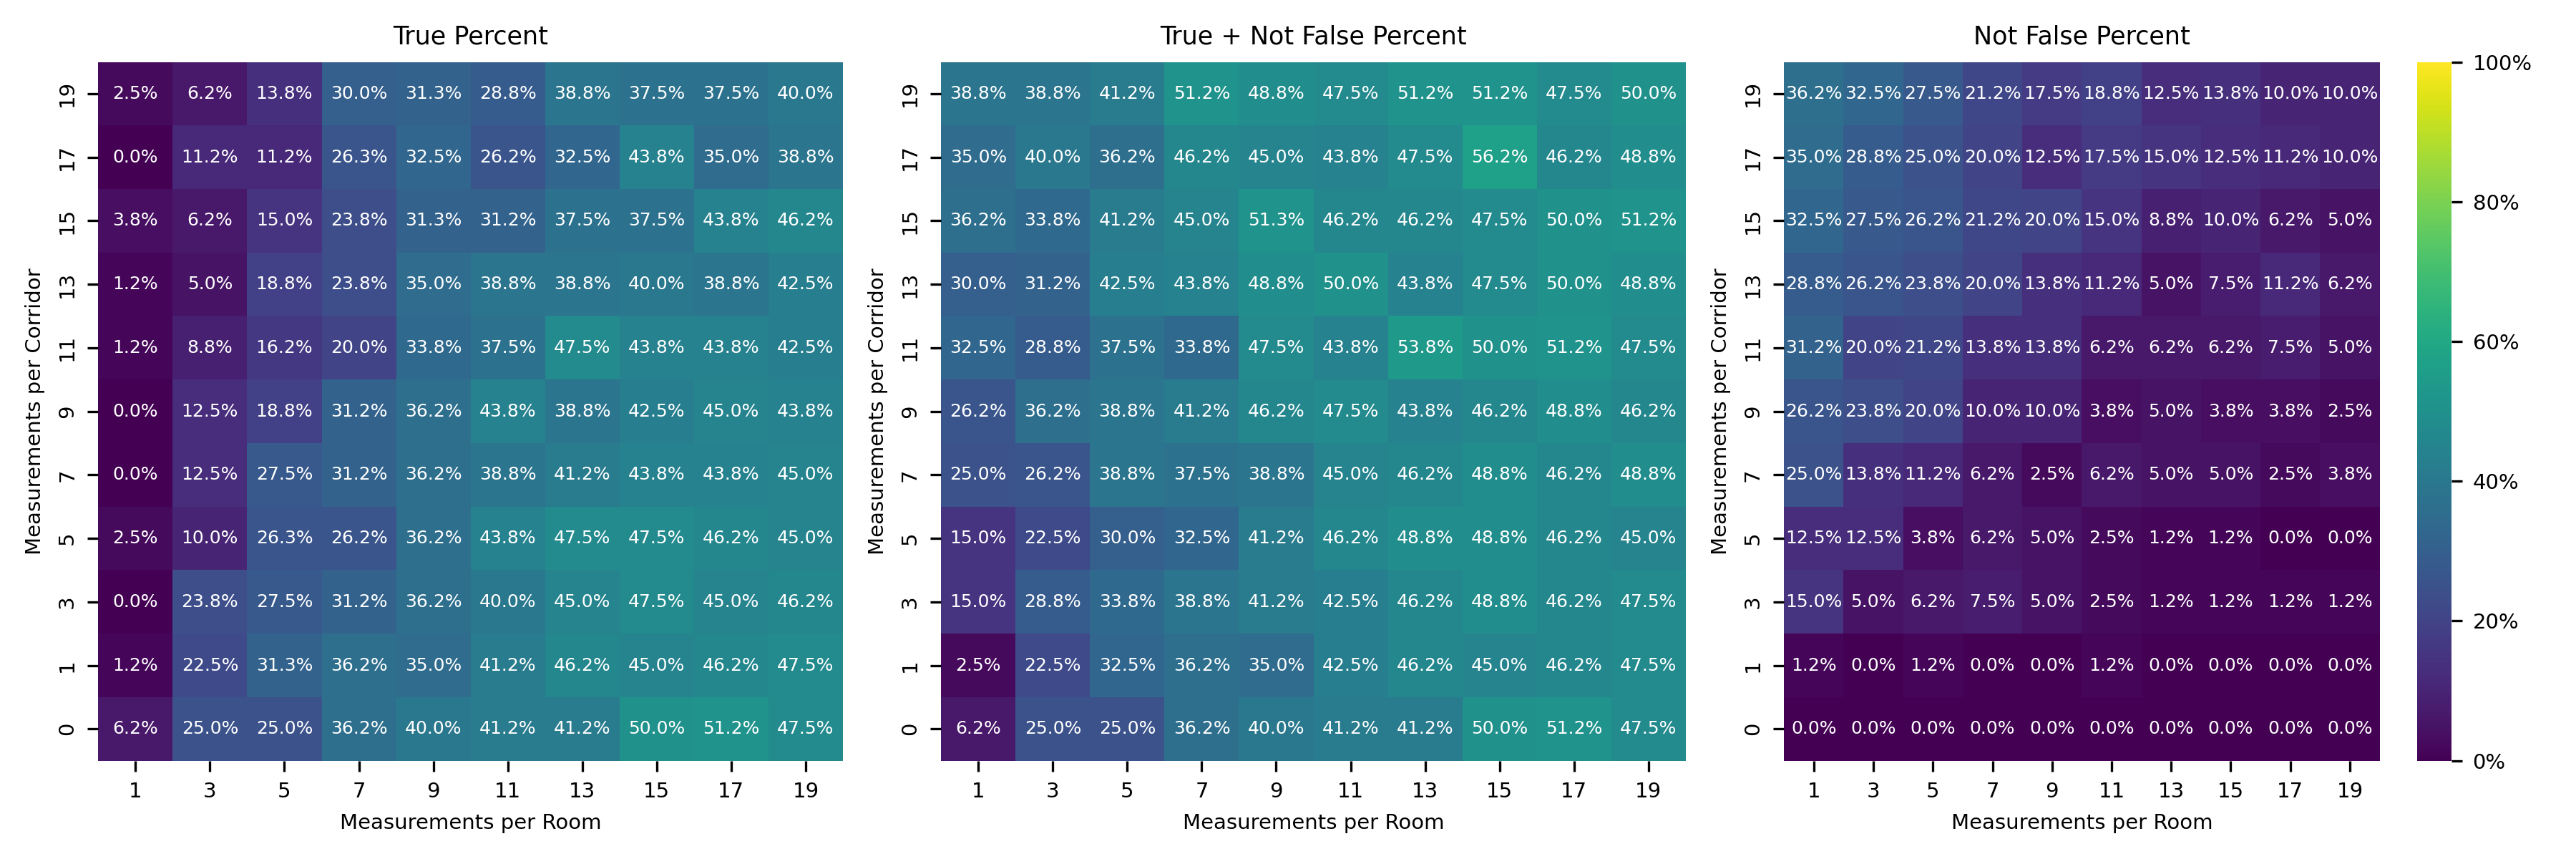
\includegraphics[width=0.8\textwidth]{images/12_corridor_01.png}
    \caption{Vergleich der Genauigkeit in Abhängigkeit der Anzahl an Messungen pro Raum und auf dem Flur}
    \label{fig:12_corridor_01}
\end{figure}

Wie zu erkennen ist, steigt die Anzahl der korrekten Vorhersagen tendenziell mit einer zunehmenden Anzahl an Messungen pro Raum und verringert sich mit einer zunehmenden Anzahl an Messungen auf dem Flur. Die besten Ergebnisse konnten dabei erzeilt werden, wenn in jedem Raum 17 Messungen und keine Messungen auf Flur verwendet wurden (51,2 \%). Bei der Betrachtung der Fälle in denen keine falsche Vorhersage getroffen wurde, weil entweder die Vorhersage korrekt war oder der Flur vorhergesagt wurde, wurden bei 15 Messungen pro Raum und 17 Messungen auf dem Flur in den meisten Fällen keine falschen Vorhersagen getroffen (56,2 \%). Von diesen 56,2 \% waren entsprachen dabei 77,96 \% einer korrekten Vorhersage und 22,04 \% einer Vorhersage des Flurs.